%Copyright 2014 Jean-Philippe Eisenbarth
%This program is free software: you can 
%redistribute it and/or modify it under the terms of the GNU General Public 
%License as published by the Free Software Foundation, either version 3 of the 
%License, or (at your option) any later version.
%This program is distributed in the hope that it will be useful,but WITHOUT ANY 
%WARRANTY; without even the implied warranty of MERCHANTABILITY or FITNESS FOR A 
%PARTICULAR PURPOSE. See the GNU General Public License for more details.
%You should have received a copy of the GNU General Public License along with 
%this program.  If not, see <http://www.gnu.org/licenses/>.

%Based on the code of Yiannis Lazarides
%http://tex.stackexchange.com/questions/42602/software-requirements-specification-with-latex
%http://tex.stackexchange.com/users/963/yiannis-lazarides
%Also based on the template of Karl E. Wiegers
%http://www.se.rit.edu/~emad/teaching/slides/srs_template_sep14.pdf
%http://karlwiegers.com
\documentclass{scrreprt}
\usepackage{listings}
\usepackage{underscore}
\usepackage[bookmarks=true]{hyperref}
\usepackage[utf8]{inputenc}
\usepackage[english]{babel}
\usepackage[acronym, toc]{glossaries}
\usepackage{graphicx}
\usepackage{calc}
\usepackage{fontawesome}
\usepackage[left = 2cm, right = 2cm]{geometry}
\usepackage{tabularx}
\usepackage{fontawesome}
\usepackage[left = 2cm, right = 2cm]{geometry}
\usepackage{tabularx}
\usepackage{enumitem}
\usepackage{indentfirst}
\usepackage{svg}
\usepackage{amsmath}
\usepackage{xcolor}
\usepackage{listings}
\usepackage{tabto}
\usepackage{pdfpages}
\usepackage{listings}
\usepackage{xcolor}
\usepackage{minted}
\usepackage{graphicx}
\usepackage{subcaption}
%Variables
 \usepackage{courier} %% Sets font for listing as Courier.
\usepackage{listings, xcolor}
\date{\today}
%\title
\usepackage{hyperref}
\hypersetup{pdfborder=0 0 0}

% custom footers and headers
\usepackage{fancyhdr}
\pagestyle{plain}
\lhead{}
\chead{}
\rhead{}
\lfoot{}
\cfoot{}
\rfoot{}
\renewcommand{\headrulewidth}{0pt}
\renewcommand{\footrulewidth}{0pt}


\newenvironment{usecase}
{\begin{flushleft}}
{
\givenscope 
\givenlevel 
\givenactor 
\givenstake
\givenpre
\givenpost
\givenms
\givenasf
\givenass
\givenast
\givenasff
\givenasfff
\givenfreq
\end{flushleft}}



%% custom commands
\newcommand{\comment}[1]{}

% \usepackage{floatrow}
% \floatsetup[table]{capposition=top}

\usepackage[utf8]{inputenc}
\usepackage[english]{babel}
\usepackage{graphicx}
\graphicspath{{images/}}
\usepackage{cite}

\usepackage{blindtext}
\usepackage{xcolor,listings}
\usepackage{textcomp}
\lstset{upquote=true}

\usepackage{subfiles} % Best loaded last in the preamble
\begin{document}

\begin{center}
  \rule{17cm}{5pt}\vskip1cm
  \begin{bfseries}
    \Large{CSCI 5410 Serverless Data Processing}\\
    \vspace{1.5cm}

    \vspace{1.5cm}

    \vspace{1.5cm}
    \Huge{Assignment 1 Report}\\
    \vspace{1.5cm}
    \LARGE{Prepared by: \\Vikram Venkatapathi - B00936916\\}
    \vspace{1.5cm}
    \vspace{1.5cm}
    \Large{Master of Applied Computer Science (Summer'23)\\
      Faculty of Computer Science\\
      Dalhousie University\\
      \vspace{3cm}
      GitLab Repo link : \url{https://git.cs.dal.ca/vikramv/csci5410-summer-23-b00936916/-/tree/A1}
    }
    %\today\\
  \end{bfseries}
\end{center}



\newpage
\phantomsection

\newpage
\phantomsection
\addcontentsline{toc}{chapter}{Table of Contents}
\tableofcontents
\newpage
\phantomsection

%\addcontentsline{toc}{chapter}{\listfigurename}

%\listoffigures

\newpage
\pagenumbering{arabic}
\part{PART A}

\newpage

\begin{flushright}
    \vspace{10cm}
    \rule{18cm}{5pt}
    \rule{18cm}{2pt}\vskip1cm
    \begin{center}
    \begin{bfseries}
        \Huge{Provide summary}\\
    \end{bfseries}
    \end{center}
    \vspace{1cm}
    \rule{18cm}{2pt}
    \rule{18cm}{5pt}
\end{flushright}
\clearpage
\chapter{Introduction}
% \label{chp:1}

The given paper titled as \textit{\textbf{Performance Evaluation of Distributed Systems in Multiple Clouds using Docker Swarm}} authored by "\textbf{N. Naik}", focuses on Docker Swarm-based Distributed System in Multiple Clouds[1].
\newline

This report attempts to review the given literature and then provides a summary.
\let\clearpage\relax

\chapter{Summary}
\label{chp:2}
The authors present a study on designing distributed systems in multiple clouds using Docker Swarm. They emphasize the benefits of multi-cloud infrastructure and discuss the challenges it entails. \textbf{Docker} is introduced as an \textbf{efficient platform for application development} through \textbf{containerization}. \textbf{Docker Swarm} [15] is highlighted as a \textbf{clustering tool} that addresses critical issues in provisioning, configuration management, load balancing, and migration. Overall, the paper provides insights into building robust distributed systems across multiple cloud environments using Docker Swarm.
\newline

% \chapter{Addressed Issue}
% \label{chp:3}
The paper specifically addresses the challenge of designing distributed systems across multiple cloud environments. It highlights the \textbf{issues} related to \textbf{provisioning, configuration management, load balancing, and} migration in such setups. The authors propose Docker Swarm as a solution to these challenges, as it provides a clustering mechanism that enables efficient application development through containerization. By leveraging Docker Swarm, the paper presents a framework for building robust distributed systems that can seamlessly operate in multi-cloud infrastructures.
\newline

% \chapter{Experiments or Studies}
% \label{chp:4}
The paper describes several experiments and studies conducted to validate the proposed framework. The authors set up a test environment consisting of multiple cloud providers\textbf{(AWS, Azure, GCP, Digital Ocean \& Softlayer)} and deployed a distributed application using Docker Swarm. They \textbf{evaluated} the \textbf{performance and scalability} of the system by \textbf{measuring response times, throughput}, and \textbf{resource utilization} under different workload conditions. Additionally, they conducted experiments to analyze the impact of network latency and node failures on the overall system performance. The \textbf{results} of these experiments demonstrated the \textbf{effectiveness} of the proposed framework in achieving efficient resource utilization, \textbf{fault tolerance}, and \textbf{seamless scalability} in multi-cloud environments.
\newline

% \chapter{Analysis and Findings}
% \label{chp:5}
The authors' analysis and findings demonstrated that their \textbf{framework improved resource utilization} in multi-cloud environments by distributing tasks effectively. The experiments showed scalability and fault tolerance, with the system adapting to workload changes and recovering from failures. \textbf{Network latency} was identified as an \textbf{influential factor}, underscoring the importance of efficient communication and task allocation. Overall, the framework proved advantageous for efficient resource management and fault tolerance in multi-cloud settings.
\newline

% \chapter{Conclusion}
% \label{chp:6}
In conclusion, the authors presented a framework for efficient resource management in multi-cloud environments. Their approach effectively distributed tasks, improved resource utilization, and demonstrated scalability and fault tolerance. The experiments highlighted the significance of network latency and emphasized the need for efficient communication and task allocation. The findings underscored the framework's ability to adapt to workload changes and recover from failures. Overall, the study showcased the advantages of the proposed framework in enhancing resource management and fault tolerance in multi-cloud settings.
\newline\newline
\textbf{My suggestions on areas of improvement:}
\newline\newline
The paper could \textbf{discuss the limitations of its experimental setup}. For example, the authors only tested the system with a small number of nodes. But according to [16], Kubernetes is a good choice, when the scale, complexity, and management of the containers increase.  Hence, It would be interesting to see how the system performs with a larger number of nodes.
\newline
The paper could \textbf{suggest potential areas for future exploration}. For example, the authors could explore how Docker Swarm could be used to build distributed systems that are more secure or more efficient.\newline
The paper could \textbf{provide alternative perspectives on the findings}. For example, the authors could compare the performance of Docker Swarm to other container orchestration tools, such as Kubernetes[17], and K3s[18]. \newline

 % \let\clearpage\relax

\newpage

\comment{
\chapter*{Revision History}

\begin{center}
    \begin{tabular}{|c|c|c|c|}
        \hline
	    Date & Version & Description & Author\\
        \hline
	     04-Mar-2021 & 1.0 & Interaction Diagram Document - Initial Release. & All\\
        \hline
	    %31 & 32 & 33 & 34\\
        % \hline
    \end{tabular}
\end{center}



\newpage
\tableofcontents
}

\comment{
\chapter{Interaction Diagram}
\begin{figure}[htp]
    \centering
    \includegraphics[width=17.5cm]{04 - Interaction Diagram/Quiz Application-2.png}
    \caption{\textbf{\textit{Login functionality - Interaction diagram}}}
    \label{fig:my_label}
\end{figure}

\begin{figure}[htp]
    \centering
    \includegraphics[width=17.5cm]{04 - Interaction Diagram/Quiz Application-1.png}
    \caption{\textbf{\textit{Quiz Application - Interaction diagram }}}
    \label{fig:my_label}
\end{figure}
}
\part{PART B}

\newpage

\begin{flushright}
  \vspace{10cm}
  \rule{18cm}{5pt}
  \rule{18cm}{2pt}\vskip1cm
  \begin{center}
    \begin{bfseries}
      \Huge{\textbf{Build, deploy, and run a Containerized Application using GCP}}\\
    \end{bfseries}
  \end{center}
  \vspace{1cm}
  \rule{18cm}{2pt}
  \rule{18cm}{5pt}
\end{flushright}
\newpage

\chapter{Procedure followed for the given experiment}
    \section{Flowchart}

\begin{figure}[htp]
    \centering
    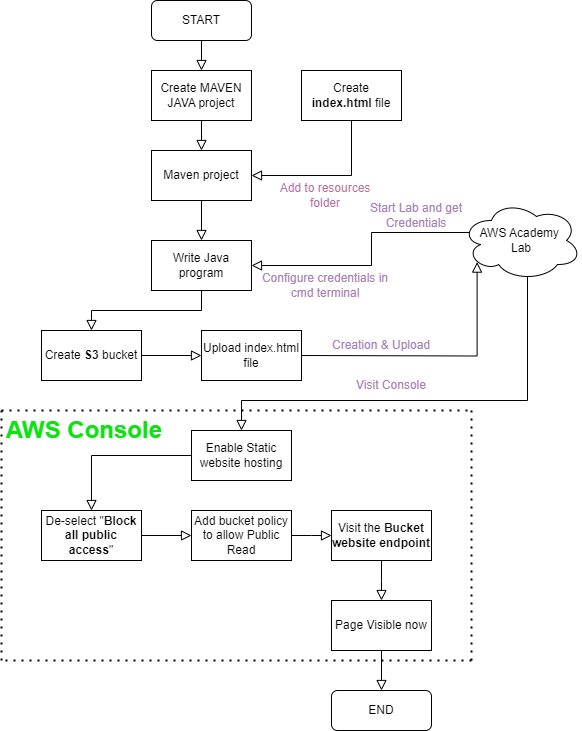
\includegraphics[scale=1, width=12cm,height=12cm]{PROBLEM 2/Flowchart.png}
    \caption{\textbf{\textit{Flowchart describing the operations that I	have performed.}}}
    \label{fig:flowchart}
\end{figure}

\section{Steps}
\subsection{Configure environment}
% \begin{enumerate}
%     \item 
% \end{enumerate}

\begin{enumerate}
    \item Create images for all the given code and front-end (i have created the front-end in React)
    \newline
    \textbf{Note}: Download the service account key from GCP IAM. In the docker file, copy the file to the container, and set it as an Environment variable as follows
    
\definecolor{backcolour}{RGB}{242, 242, 242}

\lstset{
    backgroundcolor=\color{backcolour},
    basicstyle=\small\ttfamily,
    breaklines=true,
    captionpos=b,
    frame=single,
    keywordstyle=\color{blue},
    language=,
    numbers=left,
    numbersep=5pt,
    numberstyle=\tiny\color{gray},
    showspaces=false,
    showstringspaces=false,
    showtabs=false,
    stringstyle=\color{red},
    tabsize=2
}


\begin{lstlisting}[caption={Dockerfile Code snippet}]
COPY assignment-2-390620-60700558380c.json /app/assignment-2-390620-60700558380c.json

ENV GOOGLE_APPLICATION_CREDENTIALS /app/assignment-2-390620-60700558380c.json
\end{lstlisting}
    This will allow the containers to access the collection in Firestore.
    \item Create separate repositories for all containers (3 containers: back-end; 1 container: front-end) in \textbf{Artifact Registry}.
    \item Push the images to the respective repositories
    \item Using the images, create services for all the containers, in \textbf{Cloud run} (with proper \textbf{PORT} and other configuration)
\end{enumerate}
\subsection{Control and data flow of the deployments}
\begin{enumerate}
    \item User performs registration
    \item Send a POST request to Container-1 (API: /A2/register), with all \textit{user\_data}.
    \item Registration by \textbf{Container-1}:
    \begin{enumerate}
        \item Create record in collection \textbf{"Reg"} with \textit{user\_data} (shown below)
        \lstdefinestyle{mystyle}{
    backgroundcolor=\color{backcolour},
    commentstyle=\color{codegreen},
    keywordstyle=\color{magenta},
    numberstyle=\tiny\color{codegray},
    stringstyle=\color{codepurple},
    basicstyle=\ttfamily\footnotesize,
    breakatwhitespace=false,
    breaklines=true,
    captionpos=b,
    keepspaces=true,
    numbers=left,
    numbersep=5pt,
    showspaces=false,
    showstringspaces=false,
    showtabs=false,
    tabsize=2
}

\lstset{style=mystyle}

\begin{lstlisting}[language=Python]
{
    'Name': <name>,
    'Password': <password>,
    'Email': <email>,
    'Location': <location>
}

\end{lstlisting}
        \item Return response (success/failure).
    \end{enumerate}
    \item Front-end: re-direct to \textbf{login page} after successful registration (API: /A2/login).
    \item User enters credentials.
    \item Authentication by \textbf{Container-2}
    \begin{enumerate}
        \item Fetch the respective document from the collection "Reg"  
        \item Validate credentials
        \item Return Success/Failure
    \end{enumerate}
    \item After successful authentication, 
    \begin{enumerate}
        \item If the user is logging in for the 1st time, create a \textit{session\_data} document(shown below) in the collection "state", with the user\_email as the document id.
        \lstdefinestyle{mystyle}{
    backgroundcolor=\color{backcolour},
    commentstyle=\color{codegreen},
    keywordstyle=\color{magenta},
    numberstyle=\tiny\color{codegray},
    stringstyle=\color{codepurple},
    basicstyle=\ttfamily\footnotesize,
    breakatwhitespace=false,
    breaklines=true,
    captionpos=b,
    keepspaces=true,
    numbers=left,
    numbersep=5pt,
    showspaces=false,
    showstringspaces=false,
    showtabs=false,
    tabsize=2
}

\lstset{style=mystyle}

\begin{lstlisting}[language=Python]
{
    'Online': True,
    'Offline': False,
    'Timestamp': <current_system_time>
}
\end{lstlisting}
    \item Else, just update the fields (toggle Online \& Offline, update the current timestamp of system) 
    \end{enumerate}
    \item Redirect to \textbf{session\_data page} (API: /A2/sessionData/\textless email\textgreater)
    \item Session data from \textbf{Container-3}
    \begin{enumerate}
        \item Fetch \textit{user\_data} from the collection "Reg", \textit{session\_data} from the collection "state", by matching with the \textless email\textgreater
        \item Display all the user details
        % \item Fetch all user emails from the collection "Reg"
        \item To display the other users, who are online, filter out all documents in the collection "state" where the key \textbf{"Online" is True}. (API: /A2/sessionData/usersOnline/\textless email \textgreater)
        \item Display the filtered document ids (except the current user who has logged in).
    \end{enumerate}
    \item Logout by Container-3:
    \begin{enumerate}
        \item On clicking logout, \textbf{end the current session}. (API: /A2/sessionData/\textless email \textgreater/logout)
        \item Update the \textit{session\_data} in the collection "state" (toggle Online \& Offline fields)
        \item Re-direct to the Login page.
    \end{enumerate}


\end{enumerate}

\newpage
\chapter{Screenshots}
\section{Environment setup}
% \newpage
% \subsection{Images build and push}
% \newpage
% \begin{figure}[htp]
%     \centering
%     \fbox{\includegraphics[scale=1, width=15cm,height=7.5cm]{PROBLEM 2/Screenshots/1. Setup/}}
%     \caption{\textbf{\textit{  }}}
%     \label{fig:}
% \end{figure}

\begin{figure}[htp]
    \centering
    \fbox{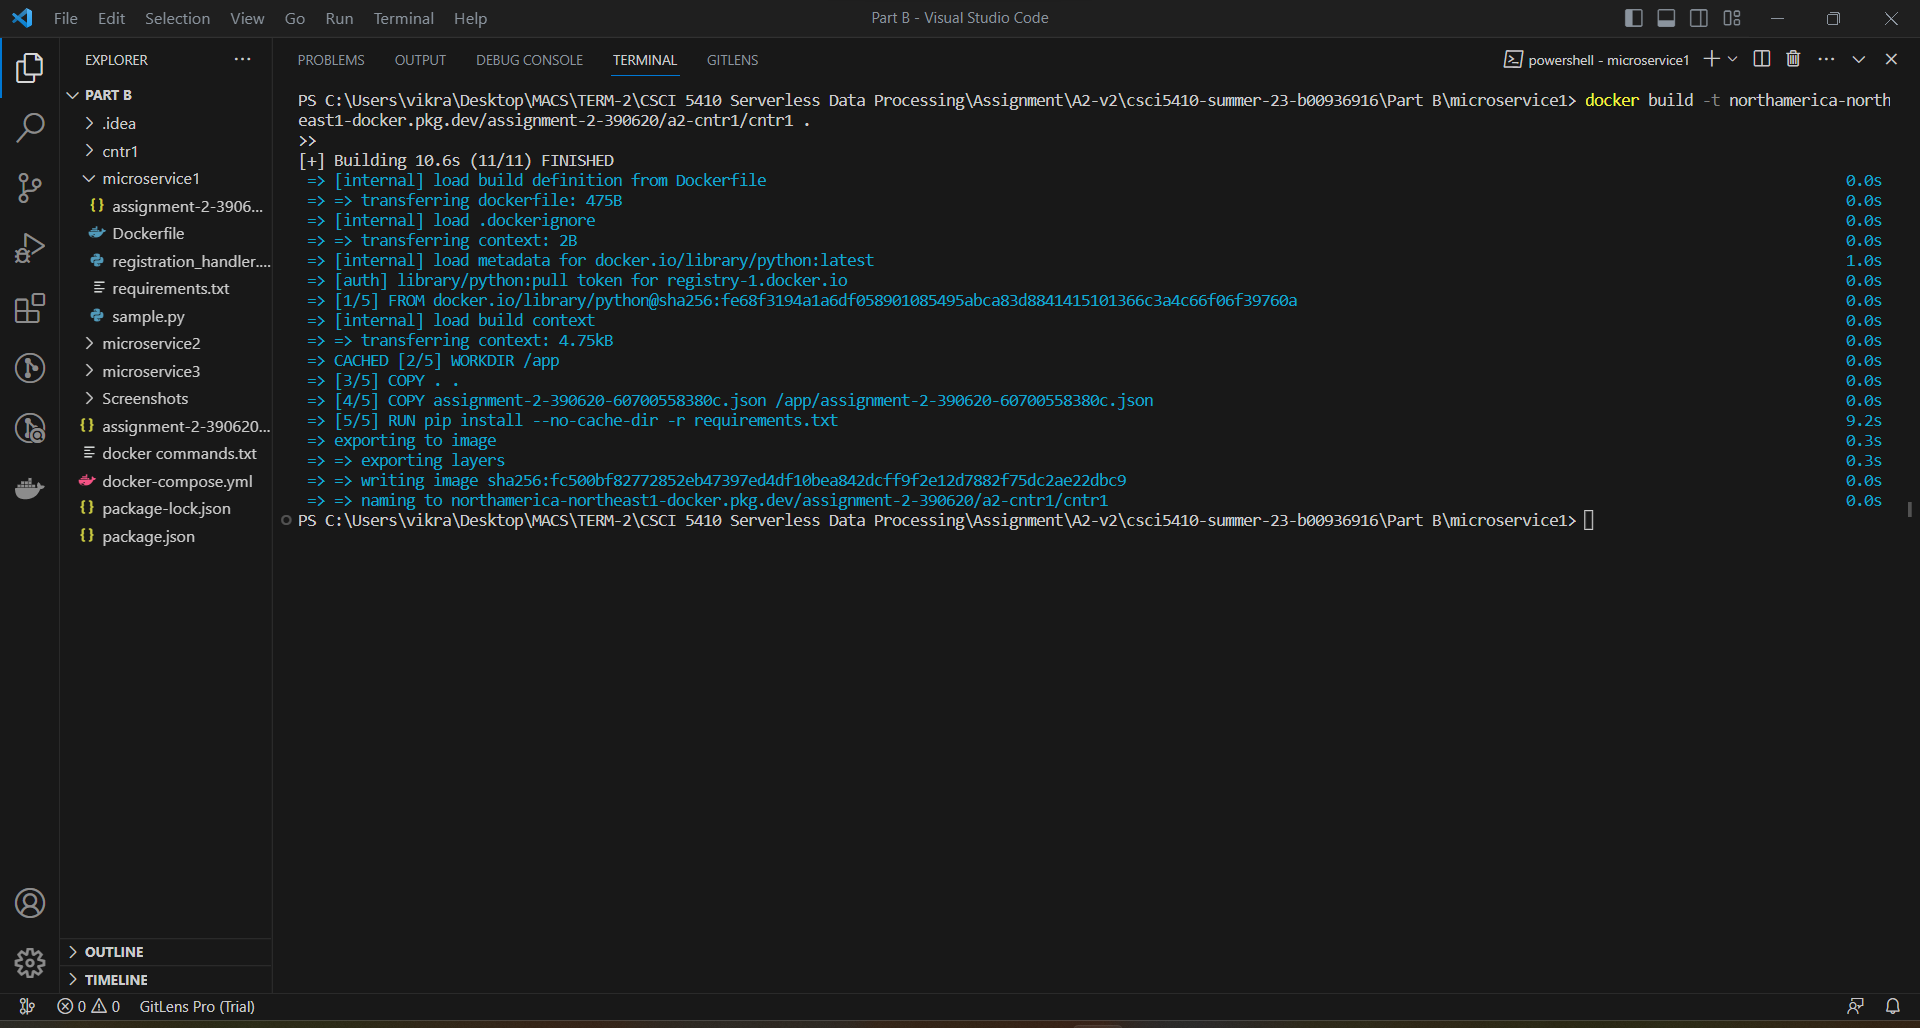
\includegraphics[scale=1, width=15cm,height=7.5cm]{PROBLEM 2/Screenshots/1. Setup/1. Image build/1.1 build cntr1.png}}
    \caption{\textbf{\textit{ Build container 1 }}}
    \label{fig:}
\end{figure}
\begin{figure}[htp]
    \centering
    \fbox{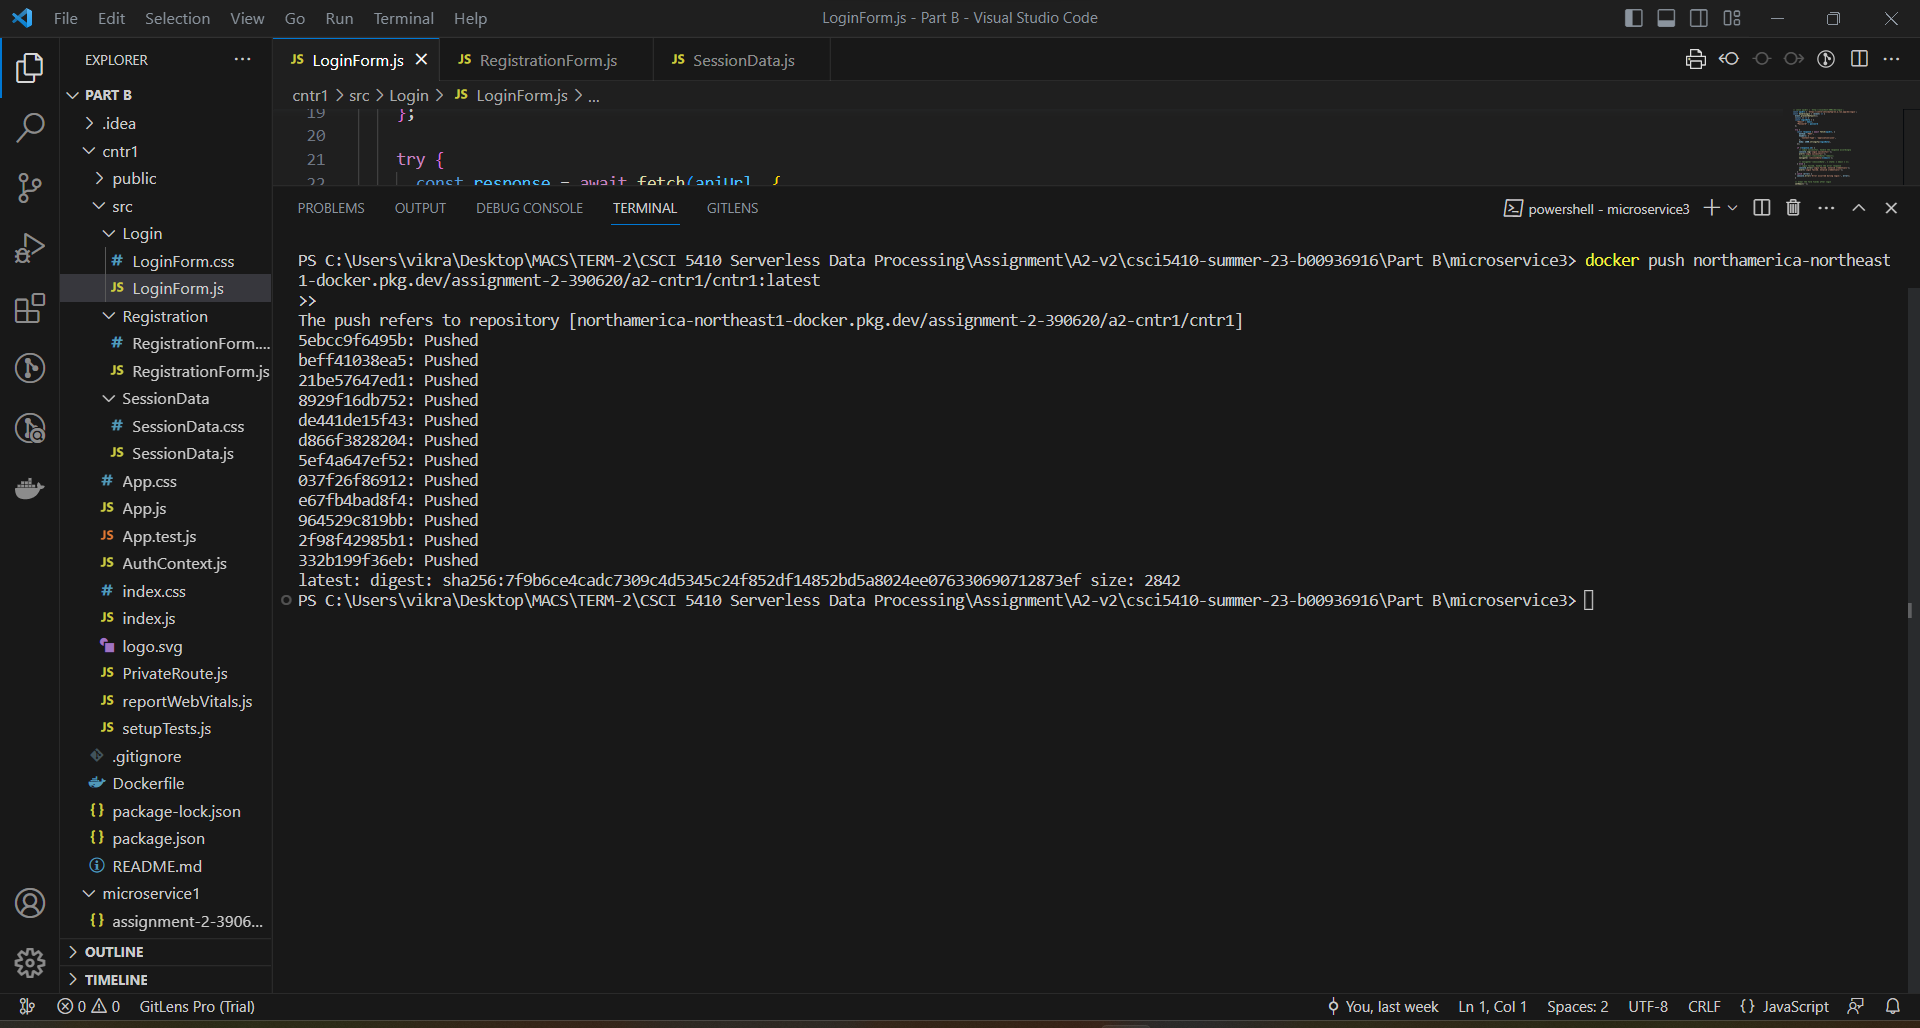
\includegraphics[scale=1, width=15cm,height=7.5cm]{PROBLEM 2/Screenshots/1. Setup/1. Image build/1.2 push cntr1.png}}
    \caption{\textbf{\textit{ Push container 1 }}}
    \label{fig:push-container-1}
\end{figure}


\begin{figure}[htp]
    \centering
    \fbox{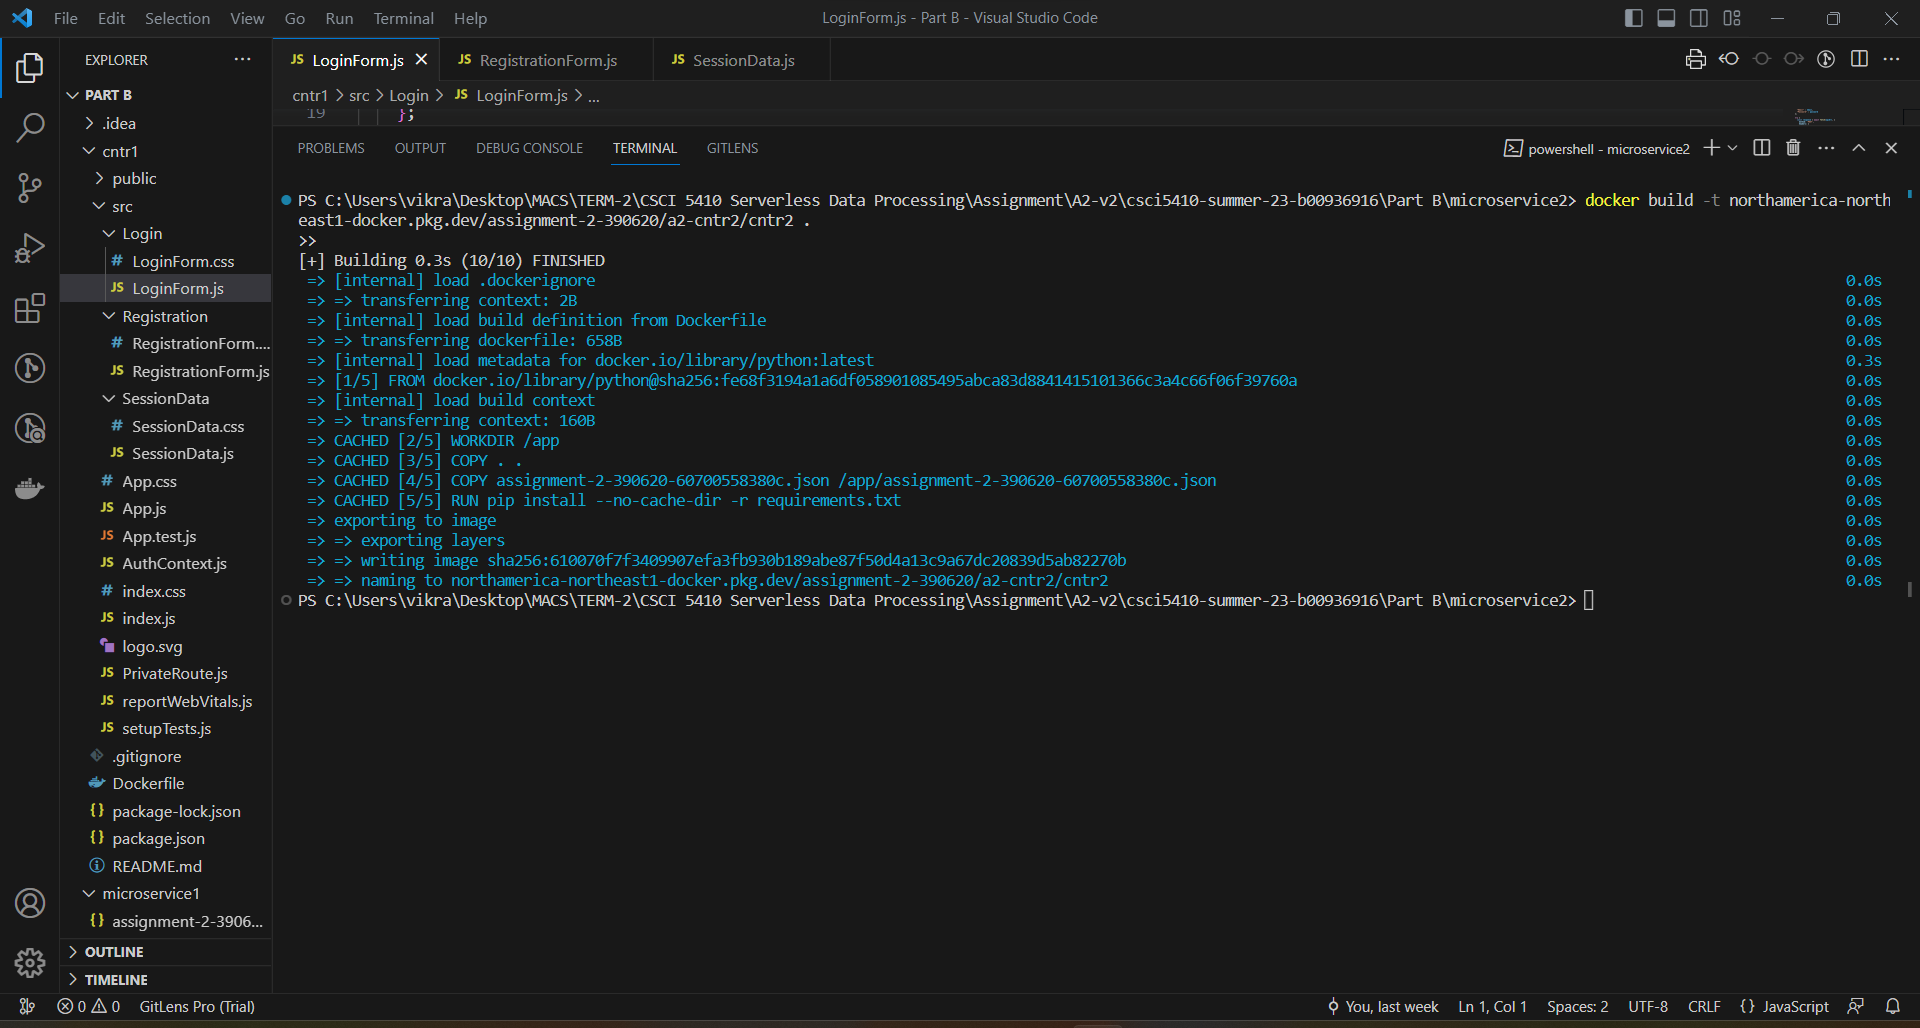
\includegraphics[scale=1, width=15cm,height=7.5cm]{PROBLEM 2/Screenshots/1. Setup/1. Image build/2.1 build cntr2.png}}
    \caption{\textbf{\textit{ Build container 2 }}}
    \label{fig:}
\end{figure}
\begin{figure}[htp]
    \centering
    \fbox{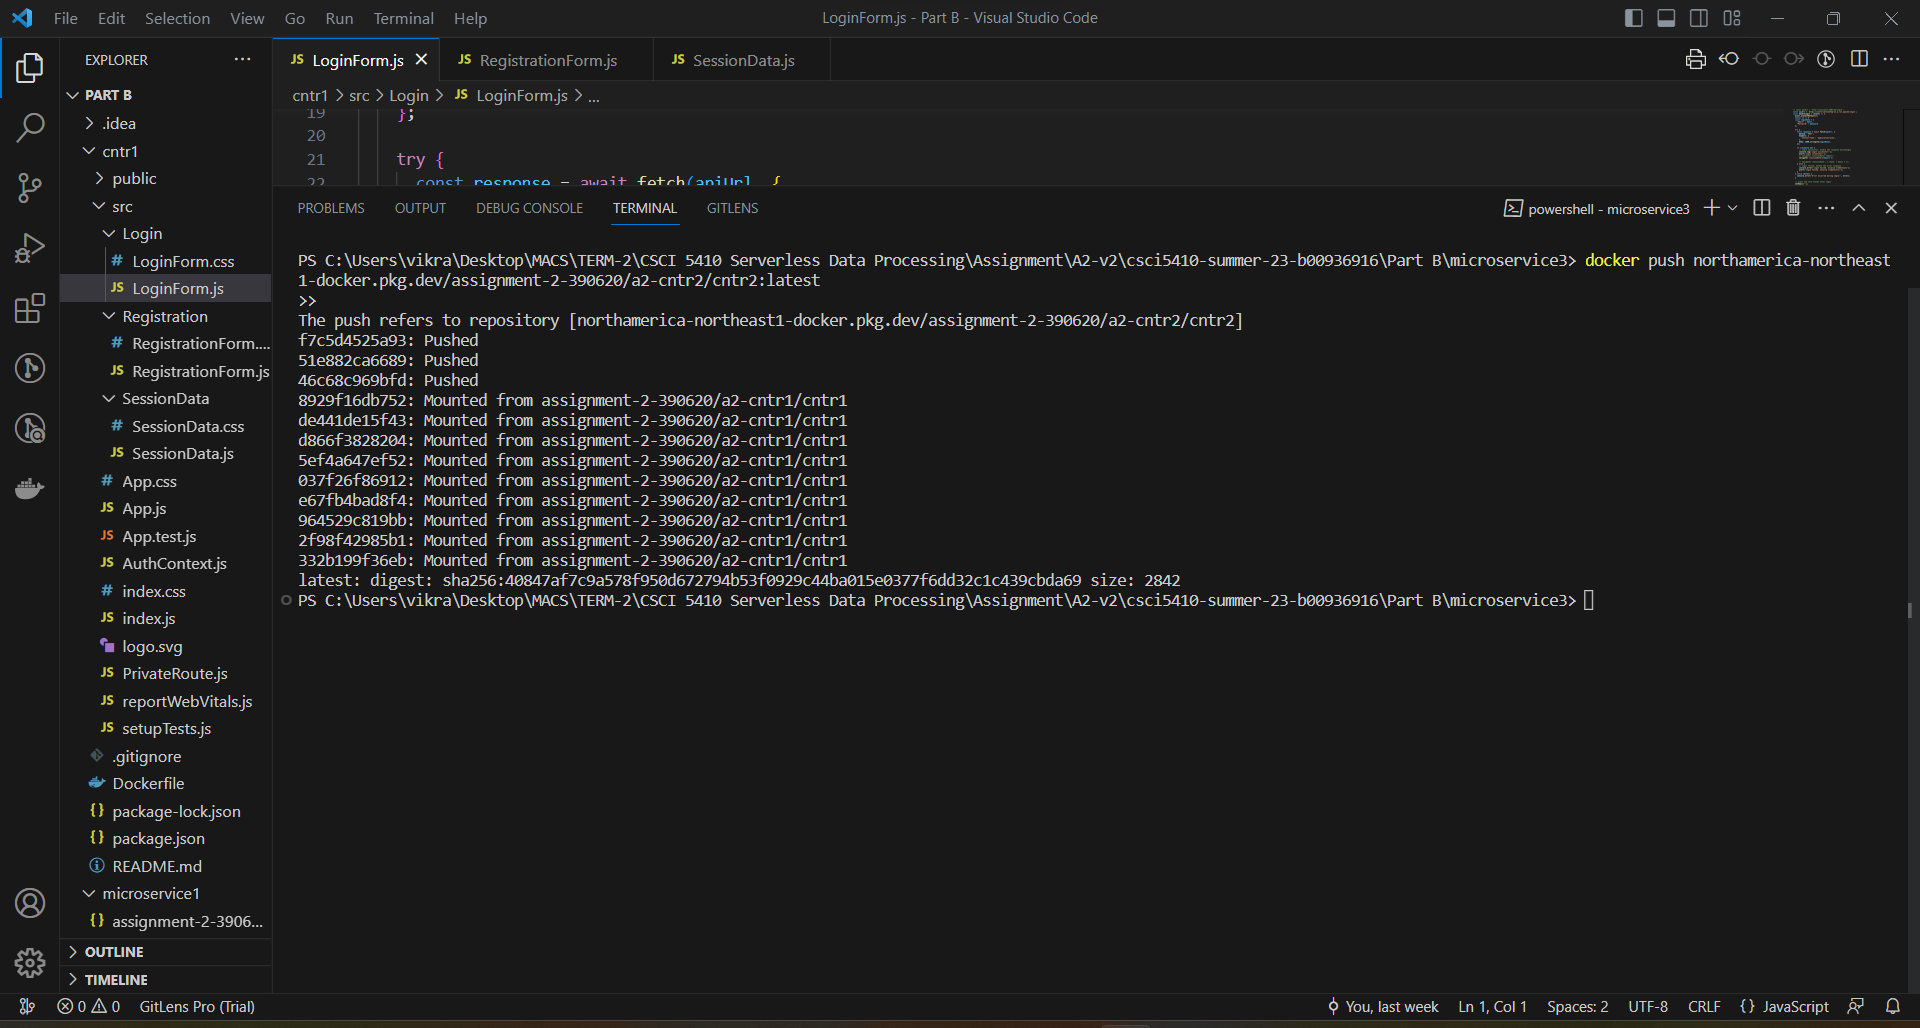
\includegraphics[scale=1, width=15cm,height=7.5cm]{PROBLEM 2/Screenshots/1. Setup/1. Image build/2.2 push cntr2.png}}
    \caption{\textbf{\textit{ Push container 2 }}}
    \label{fig:push-container-2}
\end{figure}


\begin{figure}[htp]
    \centering
    \fbox{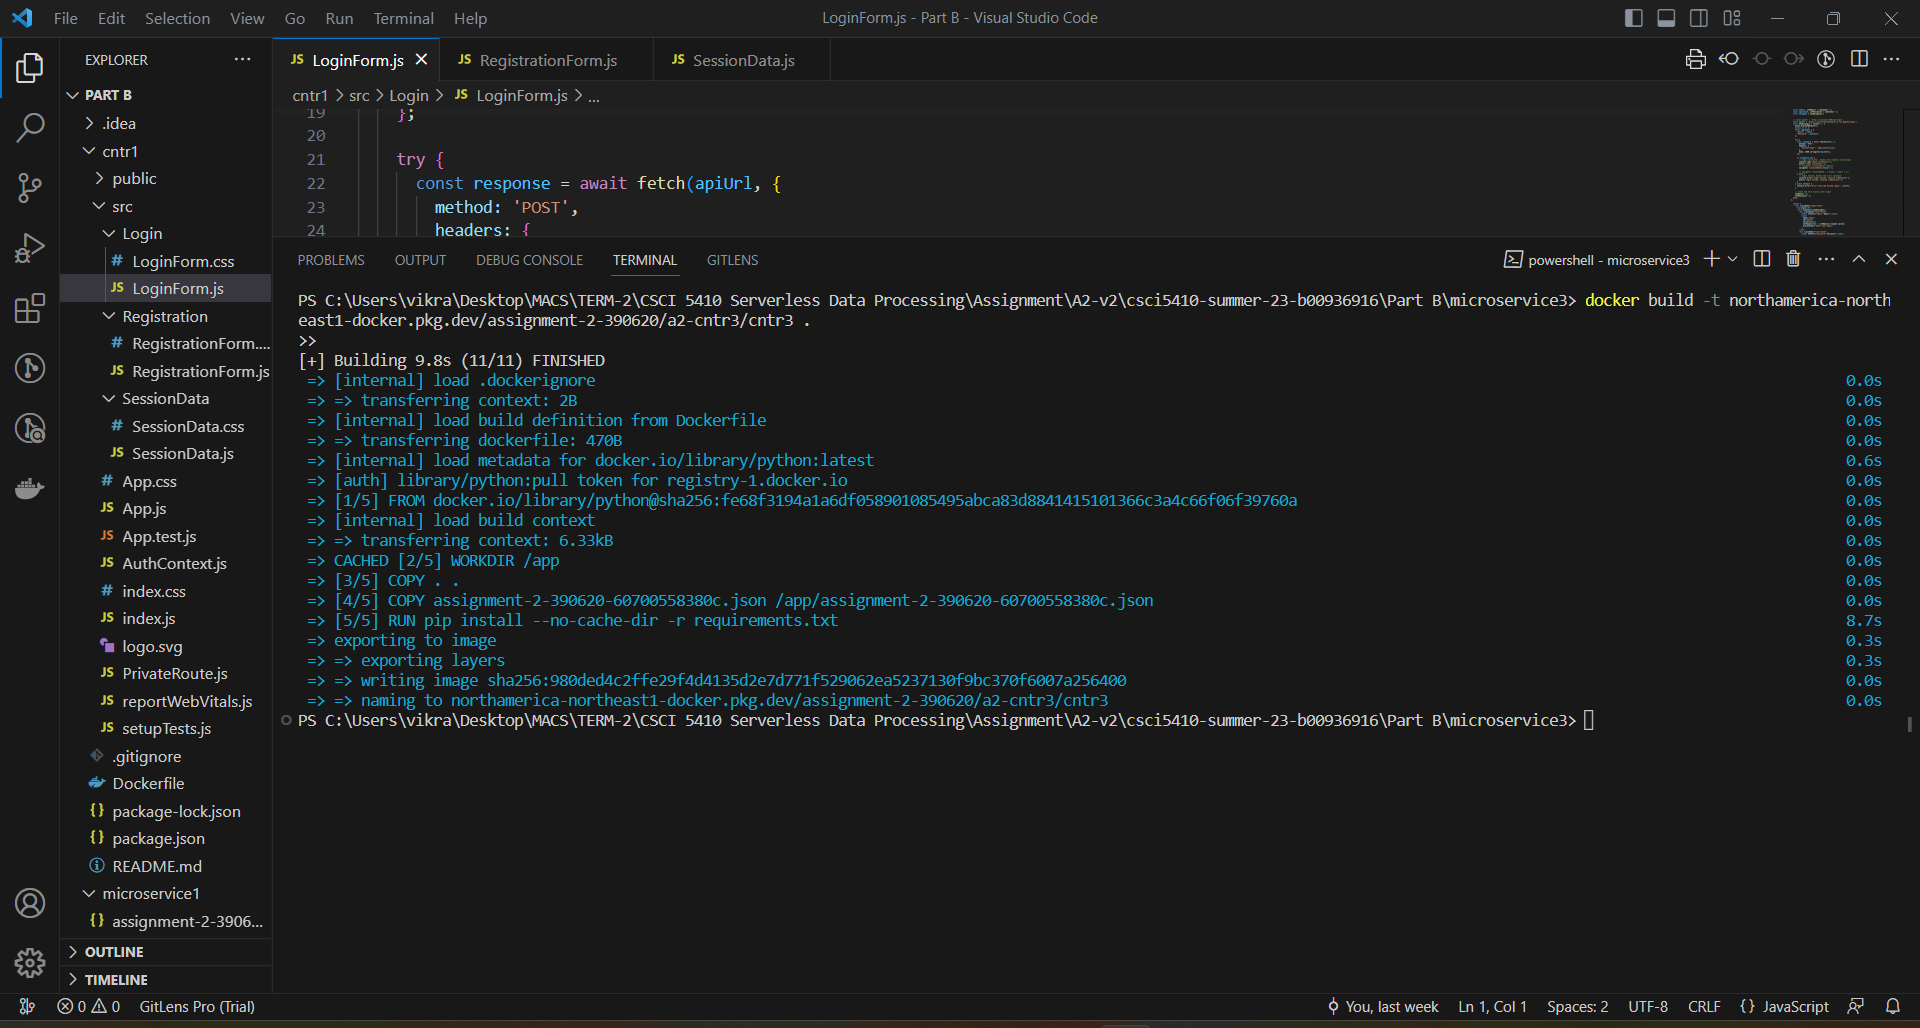
\includegraphics[scale=1, width=15cm,height=7.5cm]{PROBLEM 2/Screenshots/1. Setup/1. Image build/3.1 build cntr3.png}}
    \caption{\textbf{\textit{ Build container 3 }}}
    \label{fig:}
\end{figure}
\begin{figure}[htp]
    \centering
    \fbox{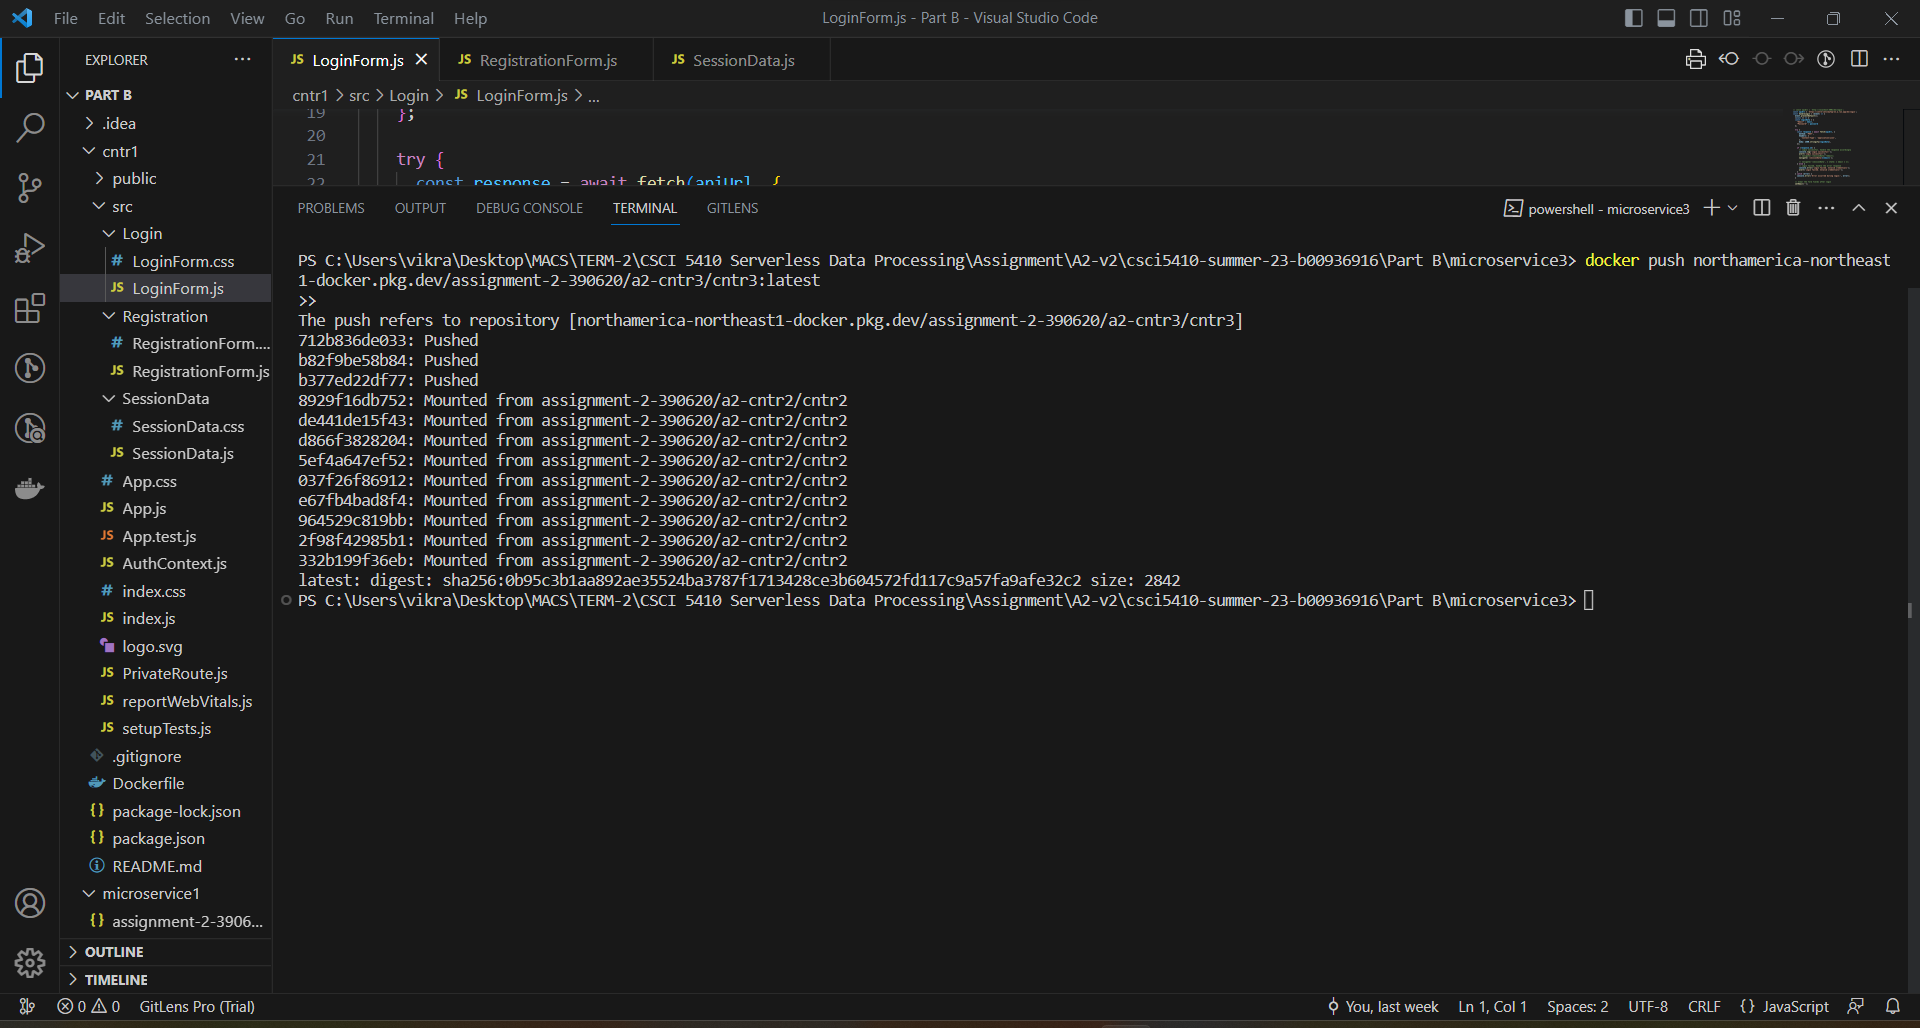
\includegraphics[scale=1, width=15cm,height=7.5cm]{PROBLEM 2/Screenshots/1. Setup/1. Image build/3.2 push cntr3.png}}
    \caption{\textbf{\textit{ Push container 3 }}}
    \label{fig:push-container-3}
\end{figure}
\begin{figure}[htp]
    \centering
    \fbox{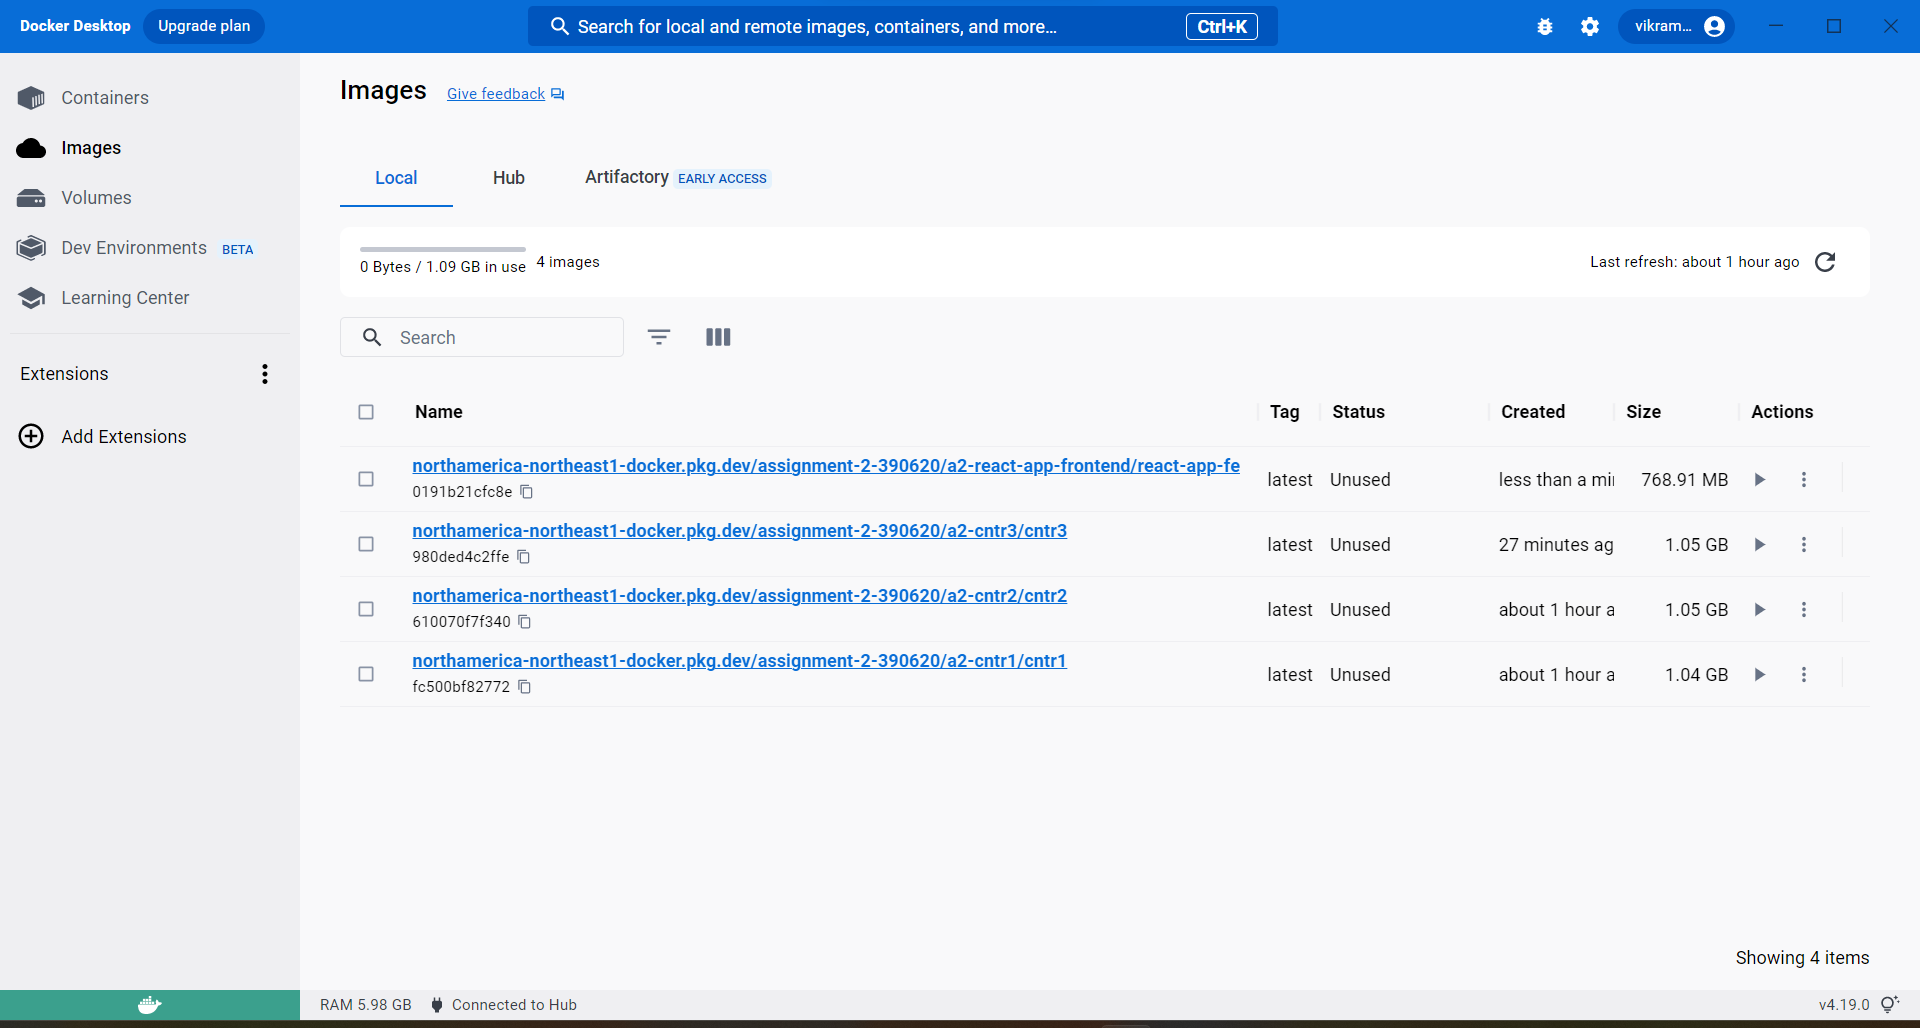
\includegraphics[scale=1, width=15cm,height=7.5cm]{PROBLEM 2/Screenshots/1. Setup/1. Image build/0. images in docker.png}}
    \caption{\textbf{\textit{ Built images listed in Docker Desktop }}}
    \label{fig:}
\end{figure}

\newpage
\subsection{Collections \& Repositories}
% \newpage
\begin{figure}[htp]
    \centering
    \fbox{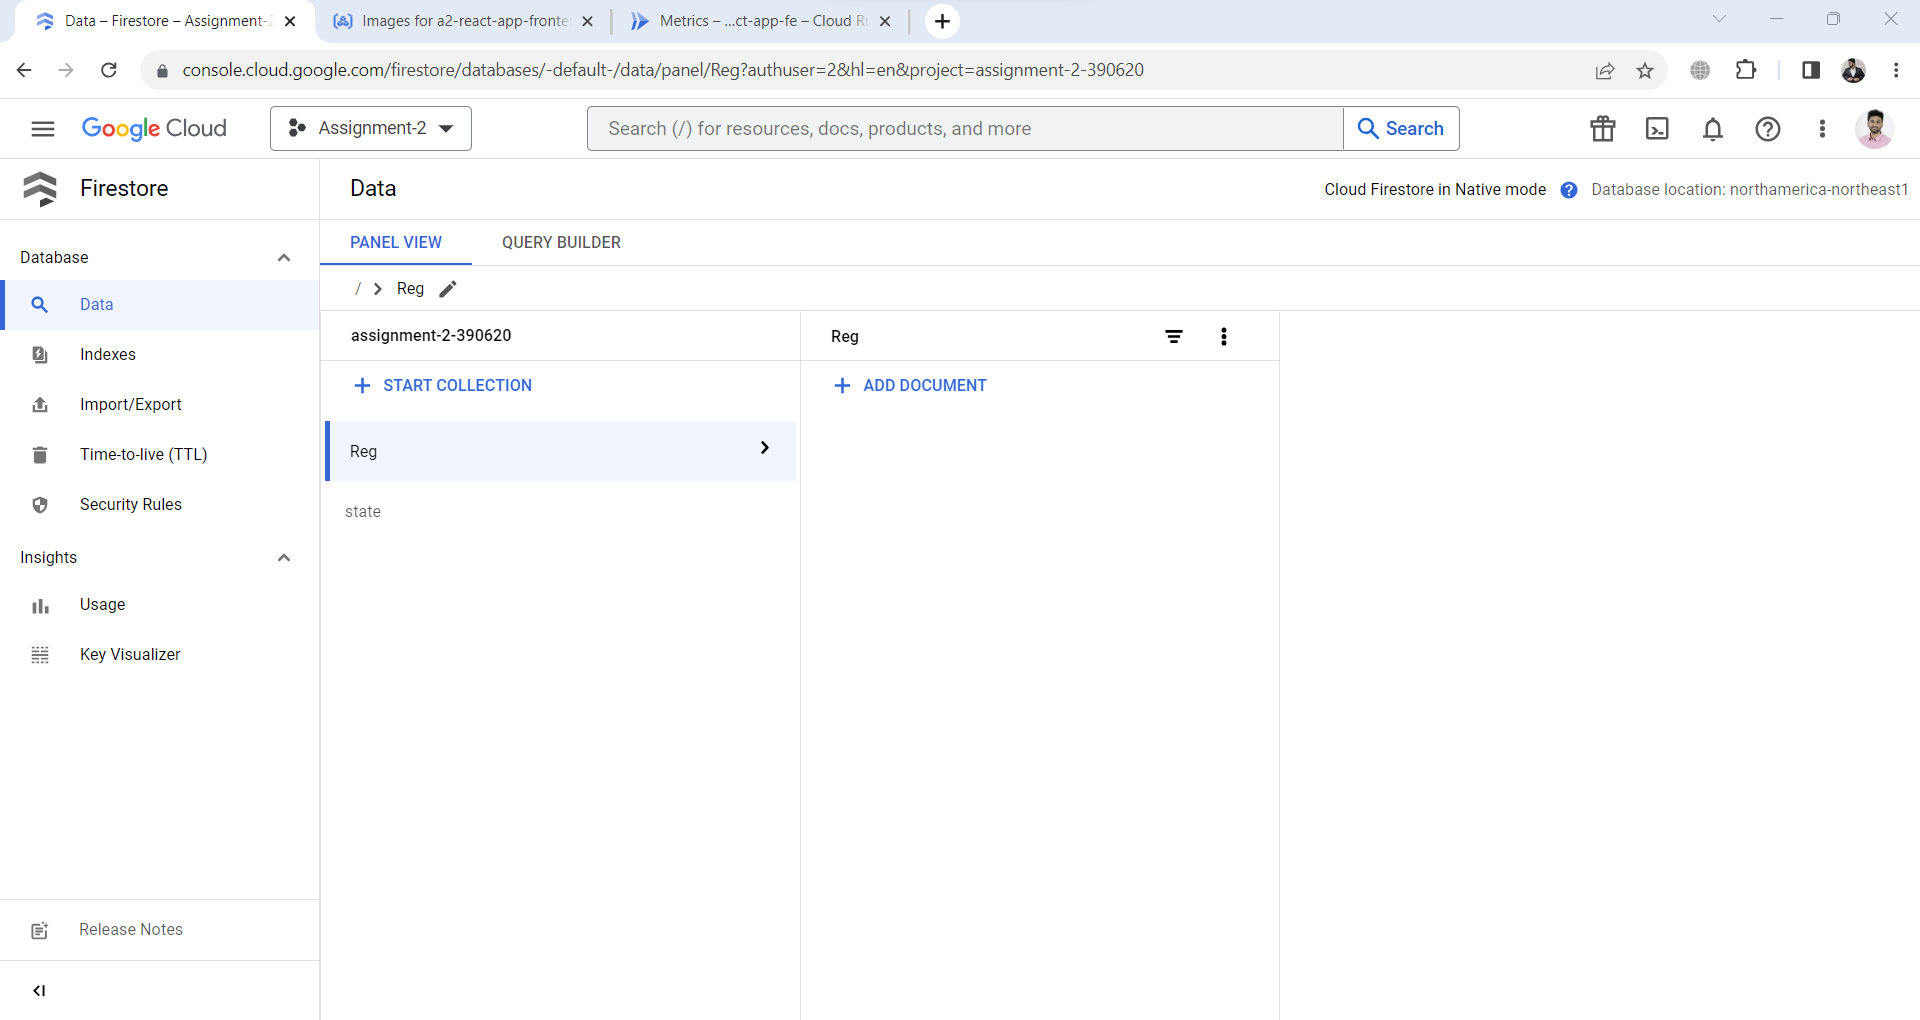
\includegraphics[scale=1, width=15cm,height=7.5cm]{PROBLEM 2/Screenshots/1. Setup/1. Empty Reg.png}}
    \caption{\textbf{\textit{ Empty collection "Reg" }}}
    \label{fig:empty-reg}
\end{figure}

\begin{figure}[htp]
    \centering
    \fbox{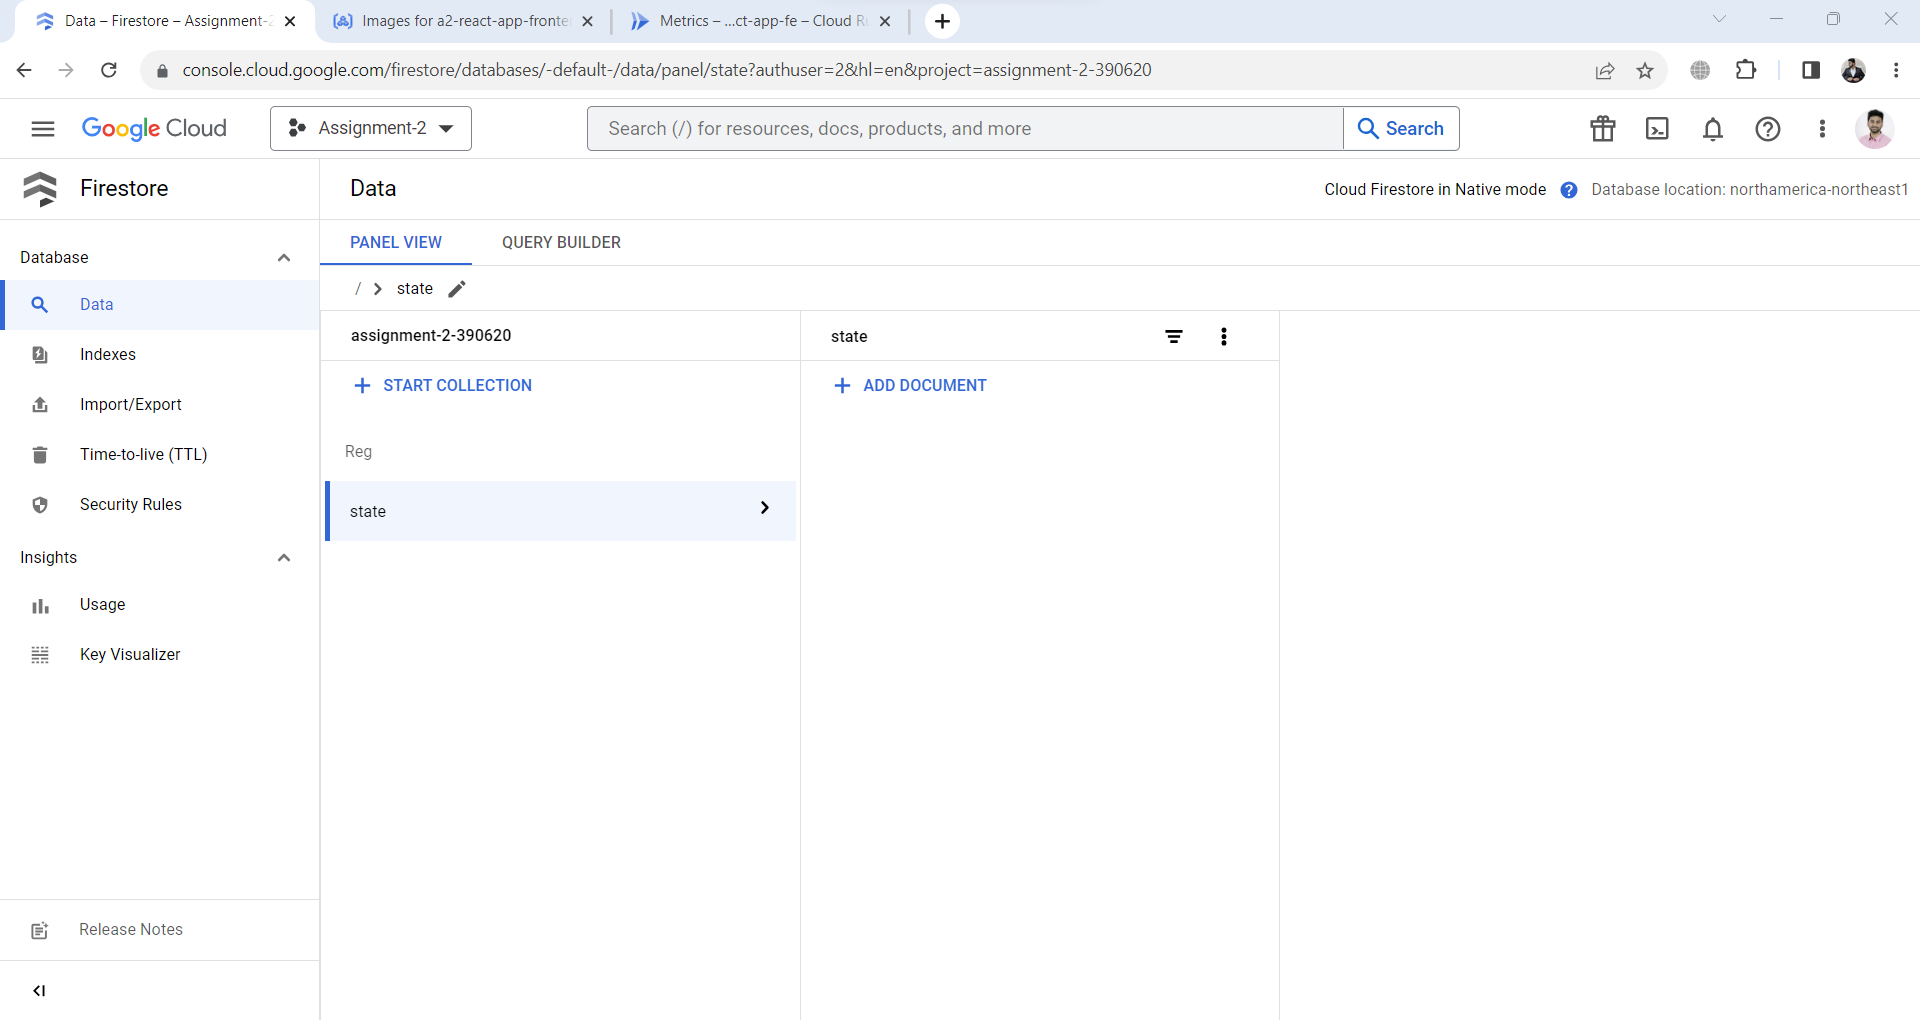
\includegraphics[scale=1, width=15cm,height=7.5cm]{PROBLEM 2/Screenshots/1. Setup/2. Empty state.png}}
    \caption{\textbf{\textit{ Empty collection "state" }}}
    \label{fig:empty-state}
\end{figure}

\begin{figure}[htp]
    \centering
    \fbox{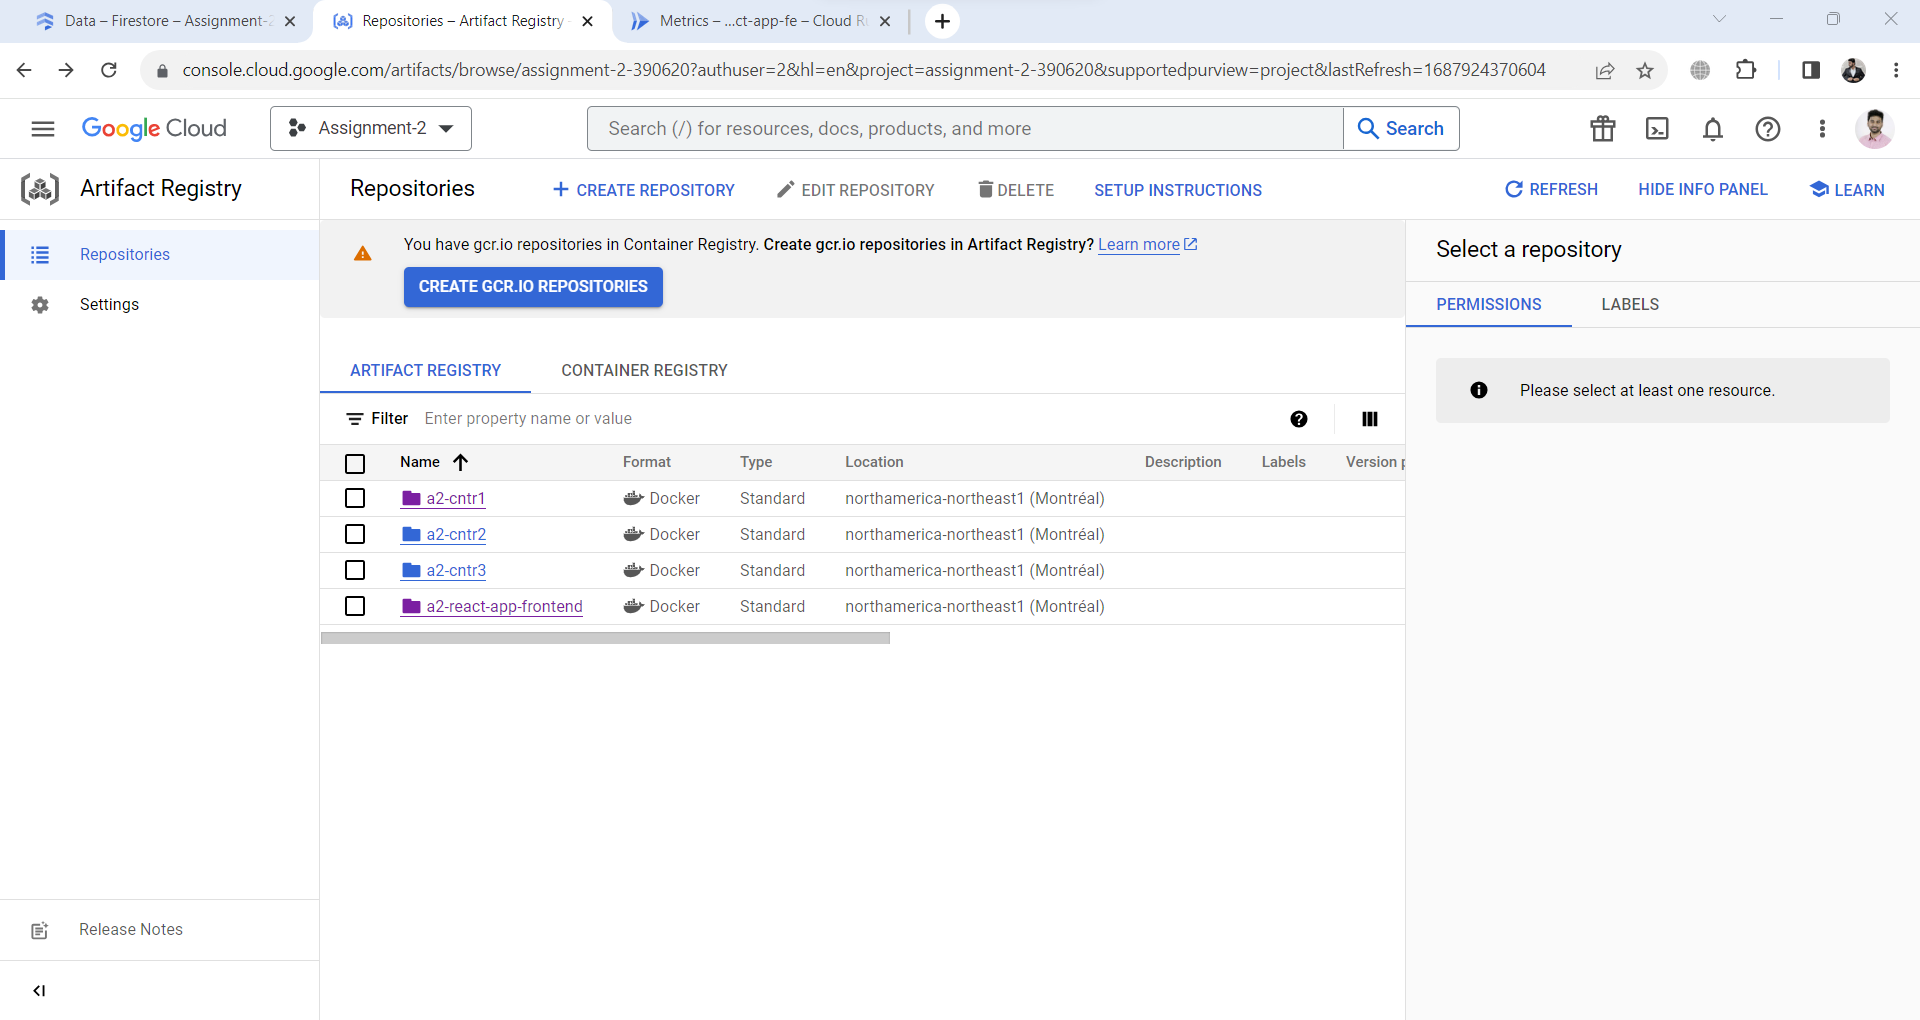
\includegraphics[scale=1, width=15cm,height=7.5cm]{PROBLEM 2/Screenshots/1. Setup/3. Artifact registry repos.png}}
    \caption{\textbf{\textit{ Artifact registry repositories }}}
    \label{fig:Artifact-registry-repo}
\end{figure}

\begin{figure}[htp]
    \centering
    \fbox{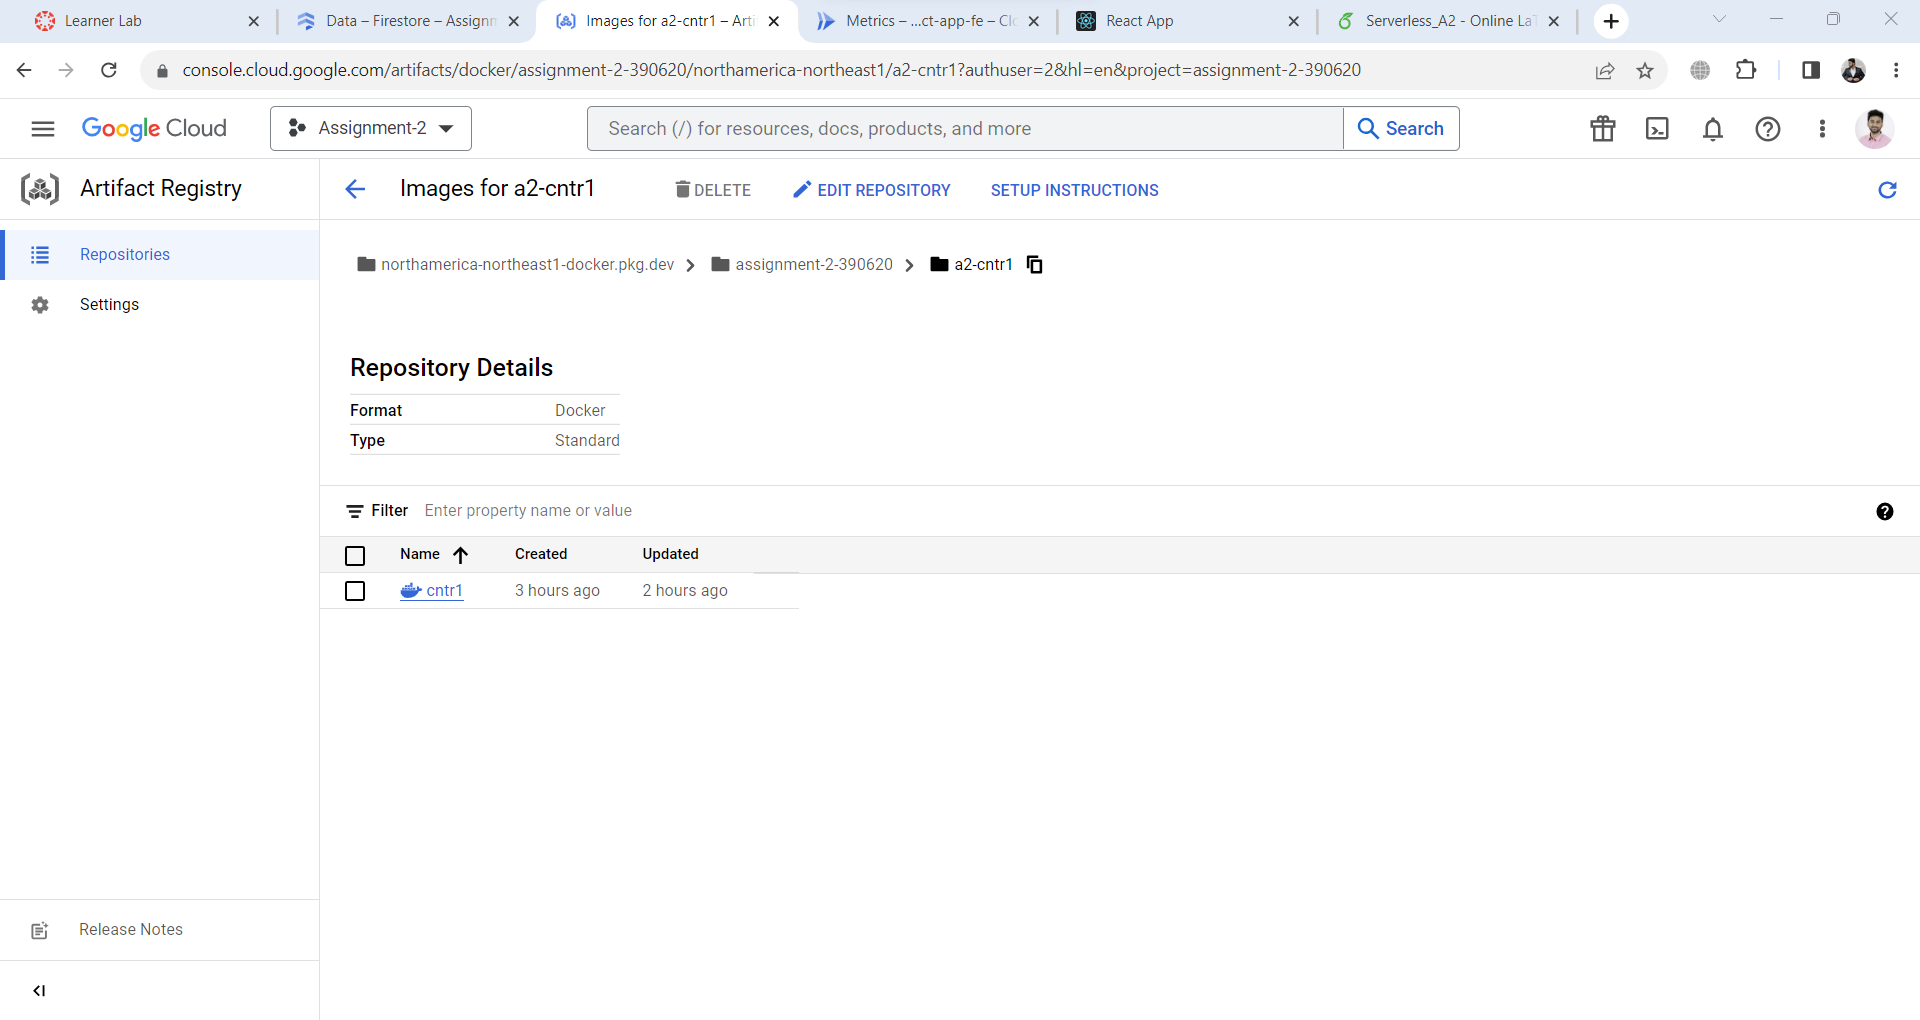
\includegraphics[scale=1, width=15cm,height=7.5cm]{PROBLEM 2/Screenshots/1. Setup/2. artifact reg repos/1. cntr1 image.png}}
    \caption{\textbf{\textit{ Artifact registry repository - container 1 }}}
    \label{fig:Artifact-registry-repo-cntr1}
\end{figure}

\begin{figure}[htp]
    \centering
    \fbox{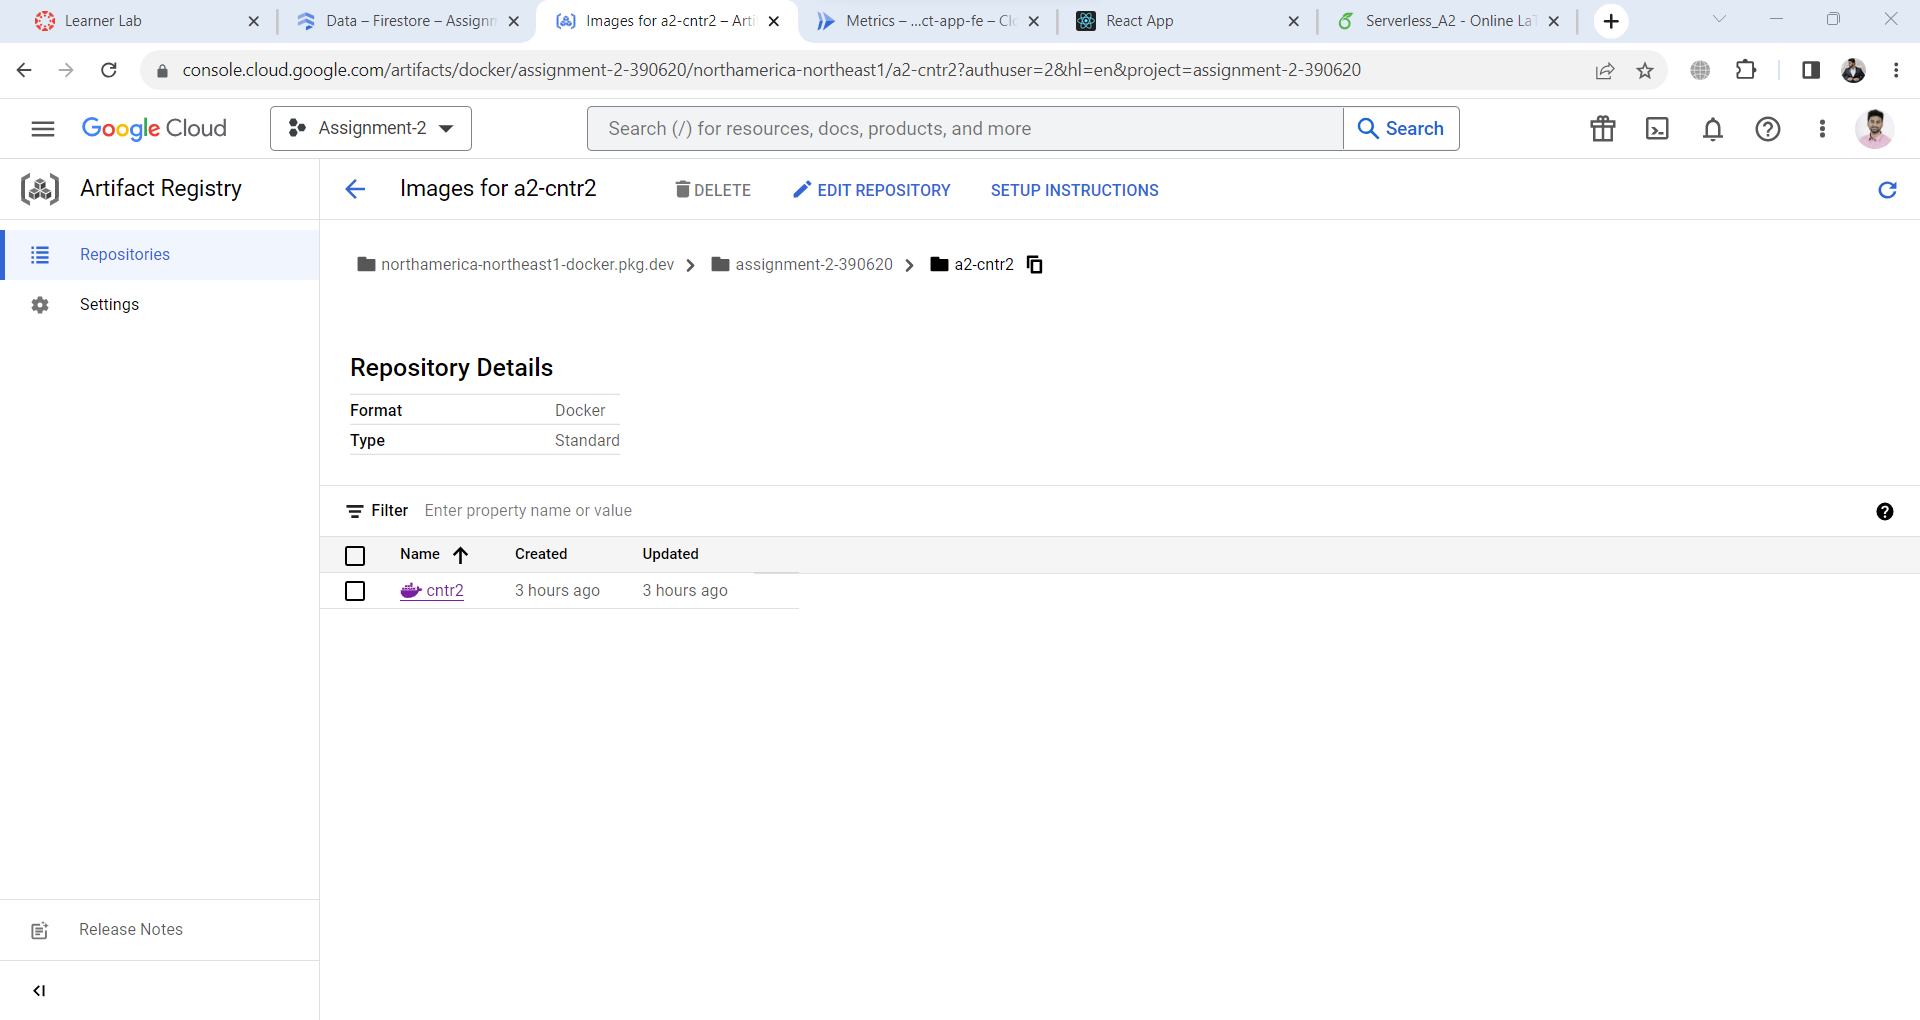
\includegraphics[scale=1, width=15cm,height=7.5cm]{PROBLEM 2/Screenshots/1. Setup/2. artifact reg repos/2. cntr2 image.png}}
    \caption{\textbf{\textit{ Artifact registry repository - container 2 }}}
    \label{fig:Artifact-registry-repo-cntr2}
\end{figure}

\begin{figure}[htp]
    \centering
    \fbox{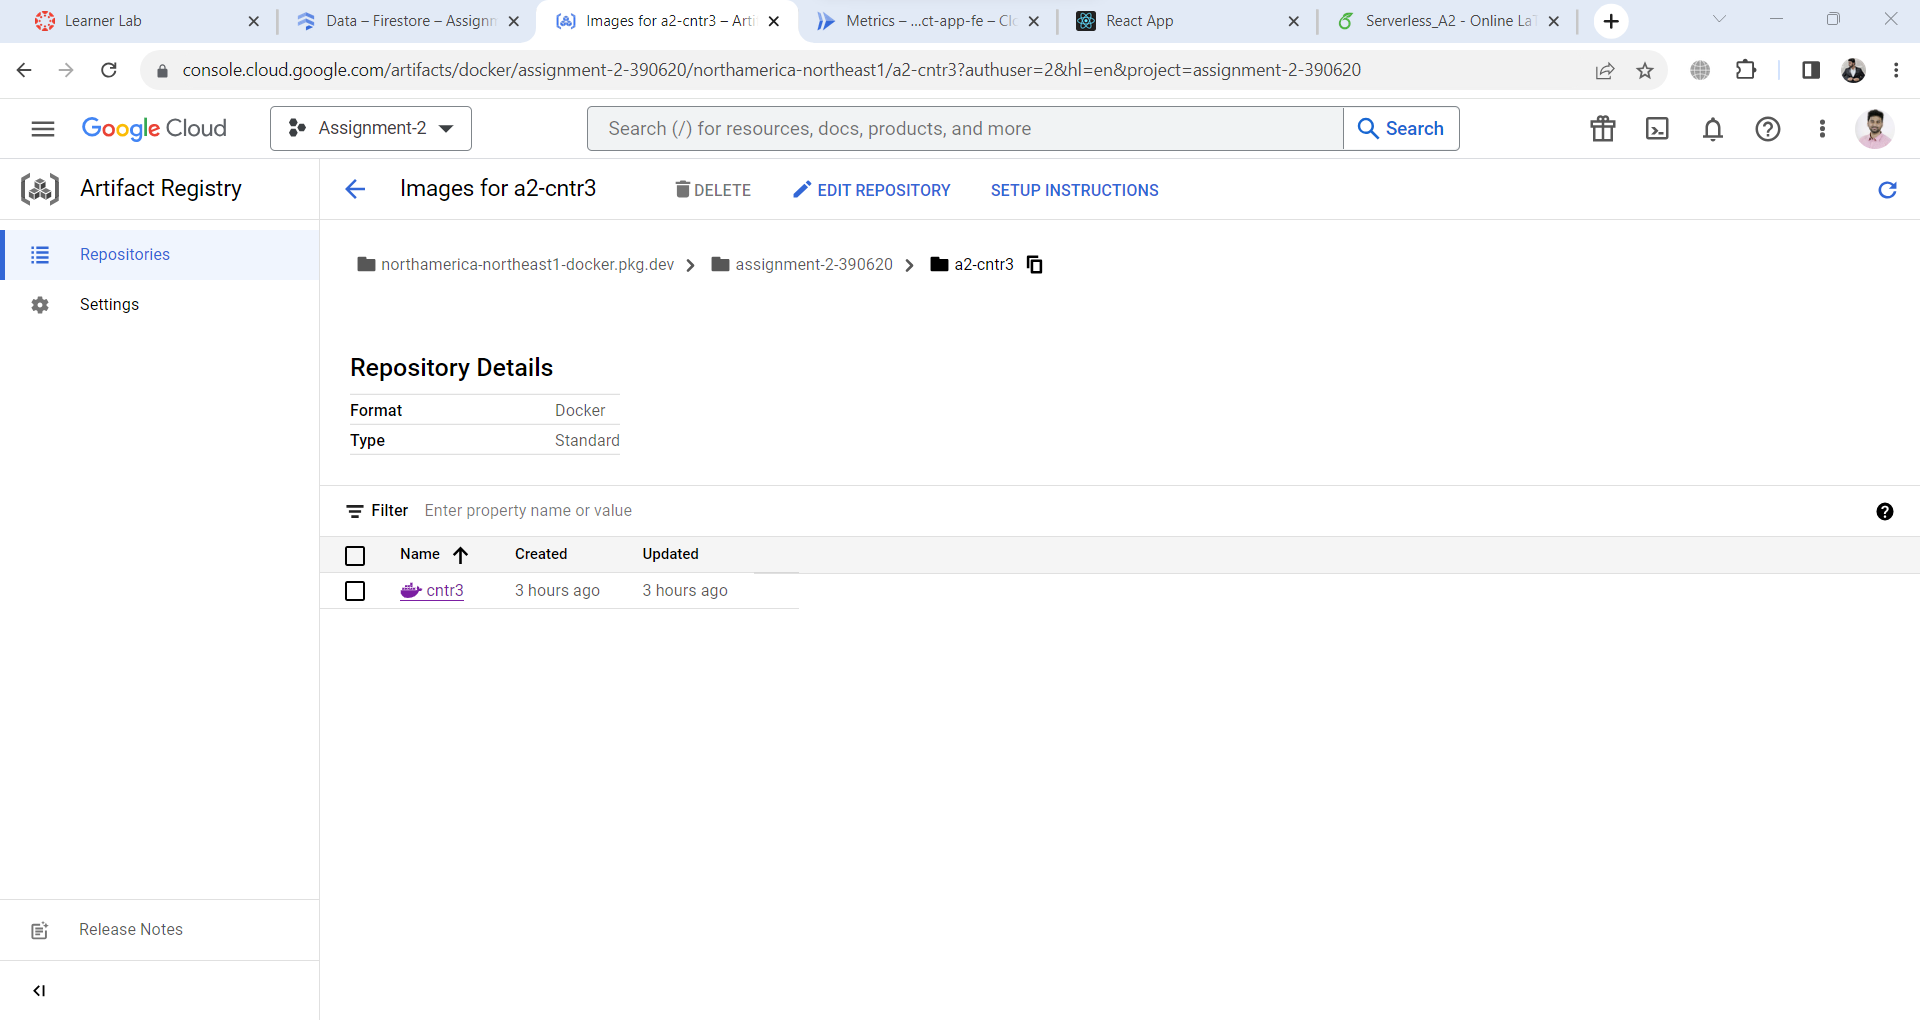
\includegraphics[scale=1, width=15cm,height=7.5cm]{PROBLEM 2/Screenshots/1. Setup/2. artifact reg repos/3. cntr3 image.png}}
    \caption{\textbf{\textit{ Artifact registry repository - container 3 }}}
    \label{fig:Artifact-registry-repo-cntr3}
\end{figure}

\begin{figure}[htp]
    \centering
    \fbox{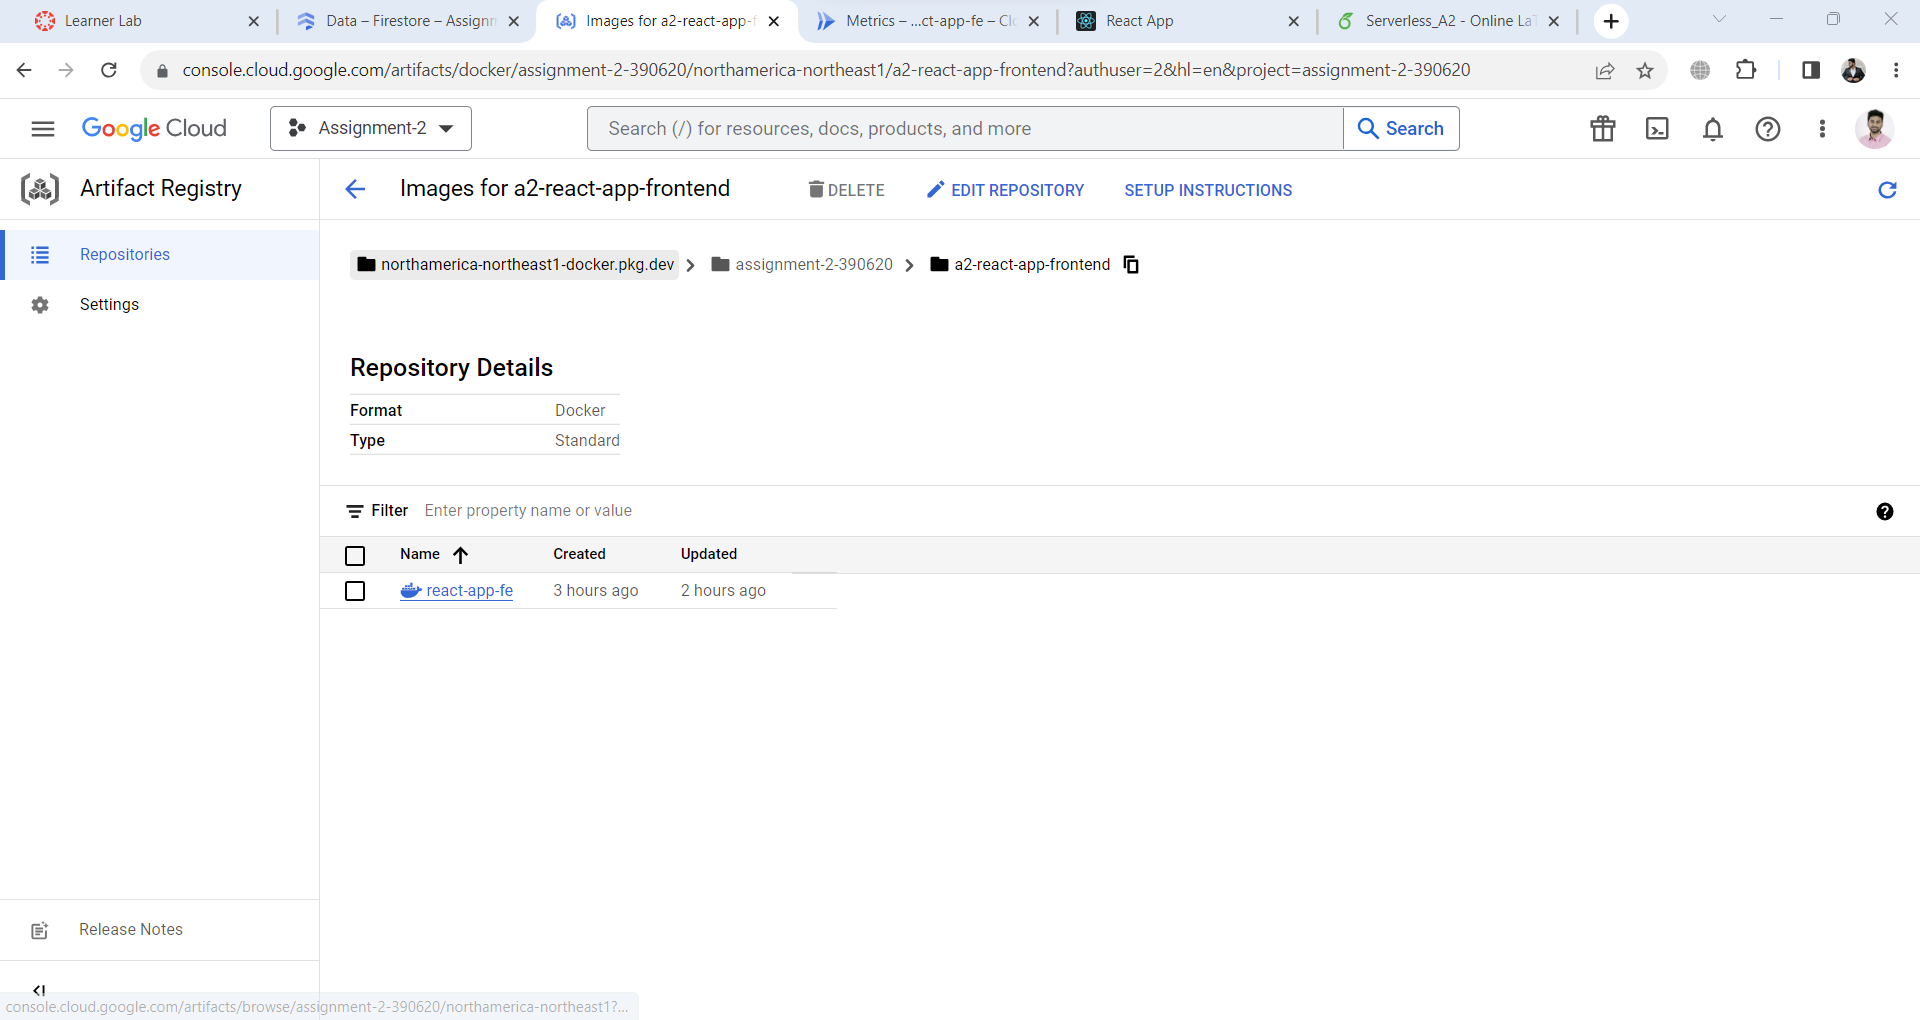
\includegraphics[scale=1, width=15cm,height=7.5cm]{PROBLEM 2/Screenshots/1. Setup/2. artifact reg repos/4. react-fe image.png}}
    \caption{\textbf{\textit{ Artifact registry repository - react-app frontend container }}}
    \label{fig:Artifact-registry-repo-cntr-fe}
\end{figure}

\begin{figure}[htp]
    \centering
    \fbox{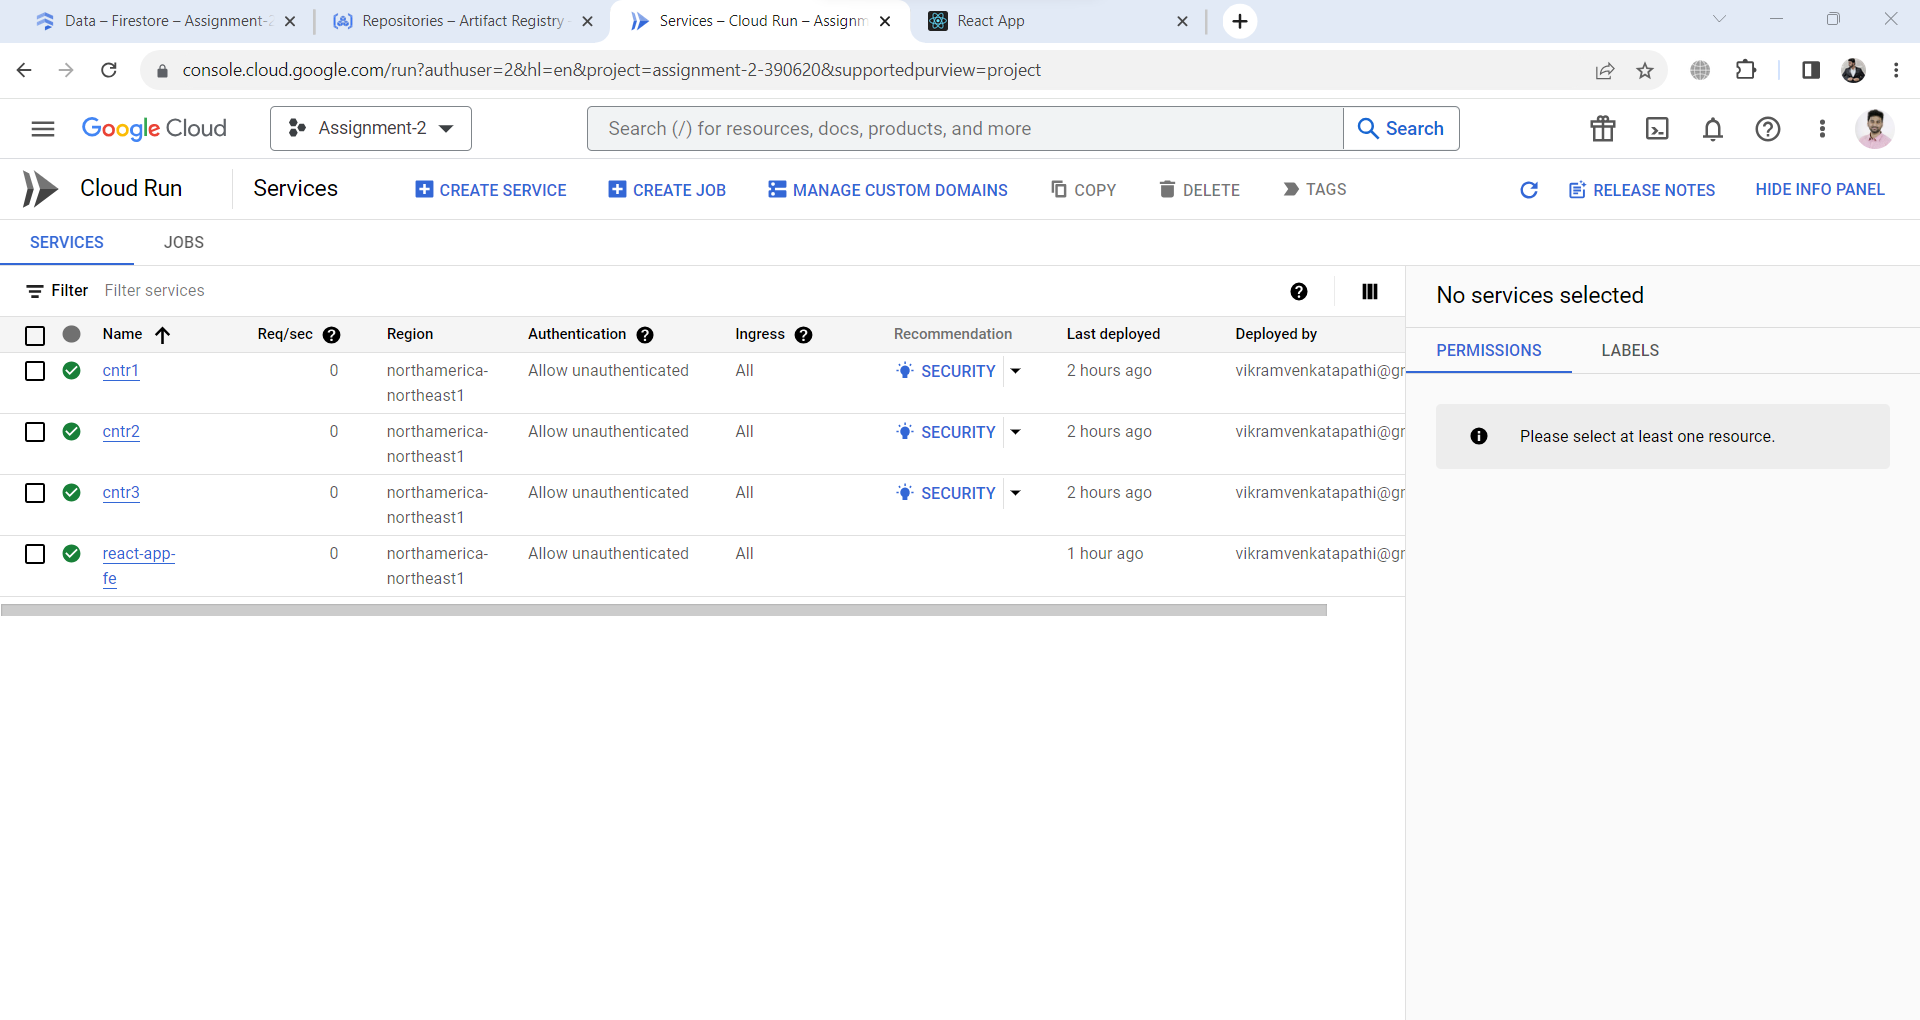
\includegraphics[scale=1, width=15cm,height=7.5cm]{PROBLEM 2/Screenshots/1. Setup/4. Cloud run - services.png}}
    \caption{\textbf{\textit{ Services created in Cloud Run }}}
    \label{fig:Cloud-Run-services}
\end{figure}

\newpage
\section{Demo}
\textbf{NOTE:}
In some of the screenshots, the URLs displayed on the front end may vary due to the process of deleting and recreating services on Cloud Run. These changes were made during the documentation process, which resulted in different URLs being assigned to the deployed containers. Please note that despite the variations in the URLs shown in the screenshots, the overall functionality and deployment process remains consistent.
\begin{figure}[htp]
    \centering
    \fbox{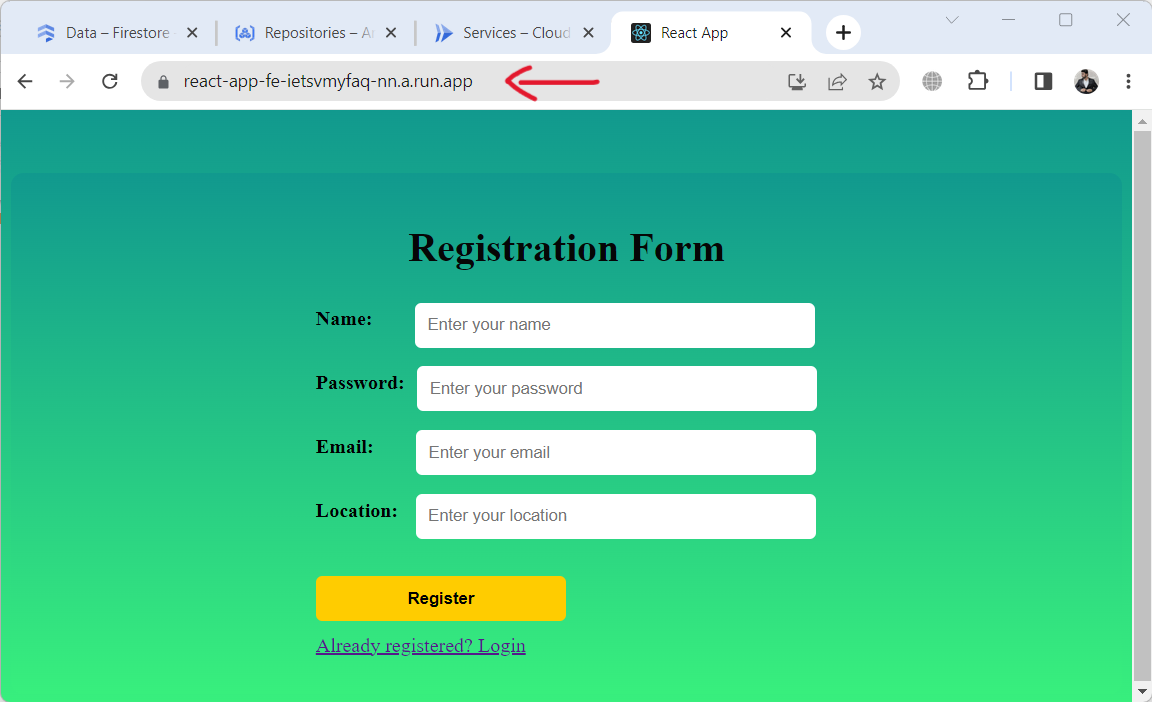
\includegraphics[scale=1, width=15cm,height=7.5cm]{PROBLEM 2/Screenshots/2. Demo/1. Reg. page.png}}
    \caption{\textbf{\textit{ Registration page }}}
    \label{fig:reg-page}
\end{figure}

\begin{figure}[htp]
    \centering
    \fbox{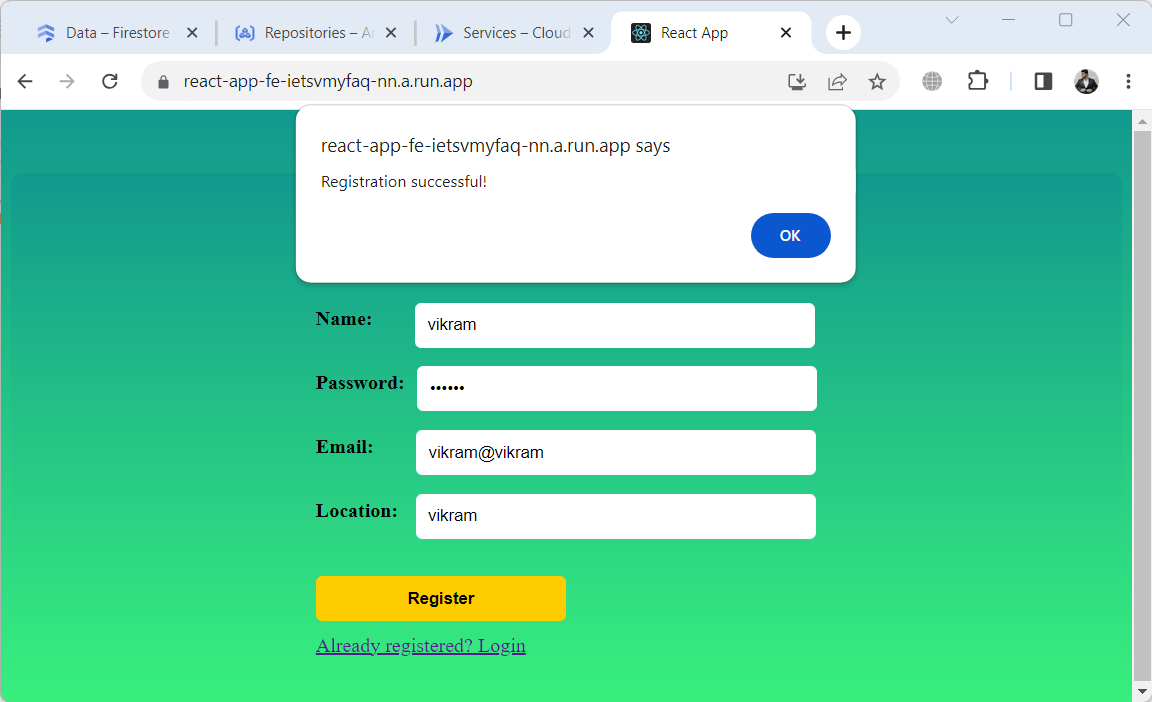
\includegraphics[scale=1, width=15cm,height=7.5cm]{PROBLEM 2/Screenshots/2. Demo/1.1 Reg success.png}}
    \caption{\textbf{\textit{ User - Vikram: Registration success }}}
    \label{fig:vikram-reg-success}
\end{figure}

\begin{figure}[htp]
    \centering
    \fbox{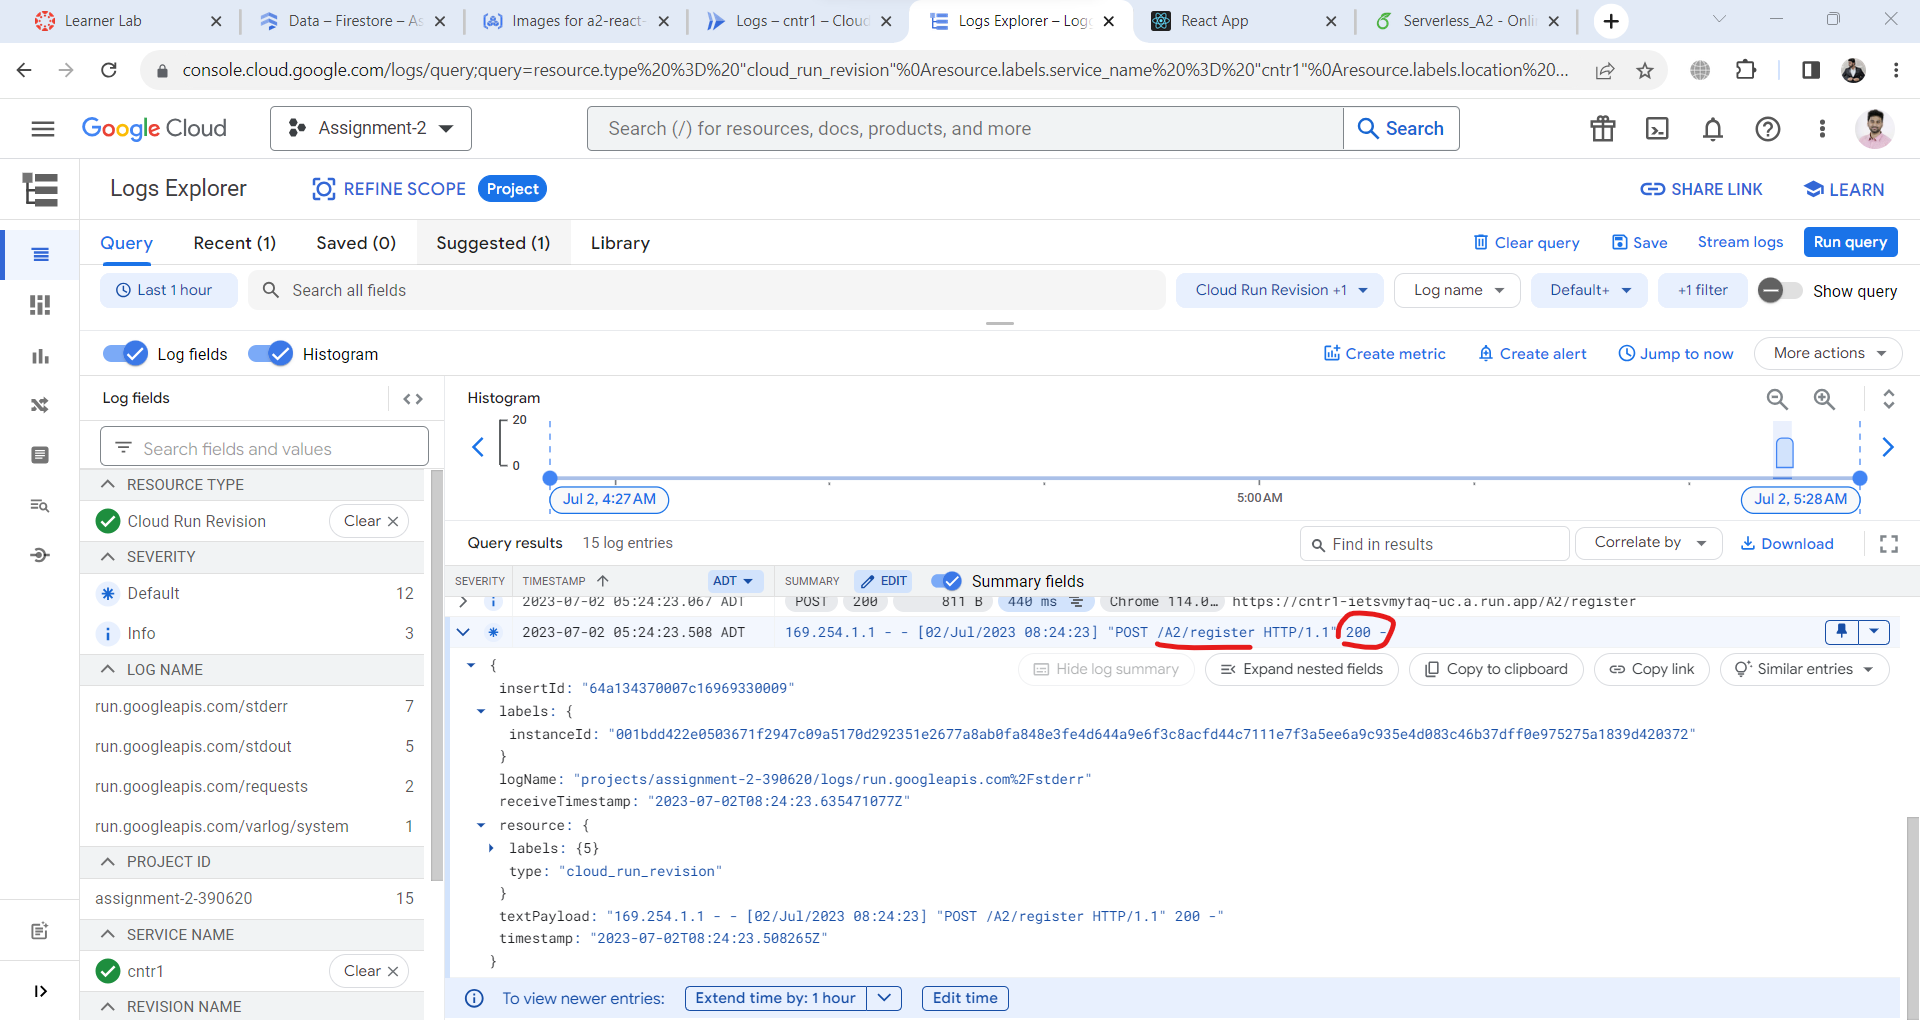
\includegraphics[scale=1, width=15cm,height=7.5cm]{PROBLEM 2/Screenshots/2. Demo/1. Logs/1. reg succes 200.png}}
    \caption{\textbf{\textit{ User - Vikram: Registration Logs}}}
    \label{fig:vikram-record-created}
\end{figure}

\begin{figure}[htp]
    \centering
    \fbox{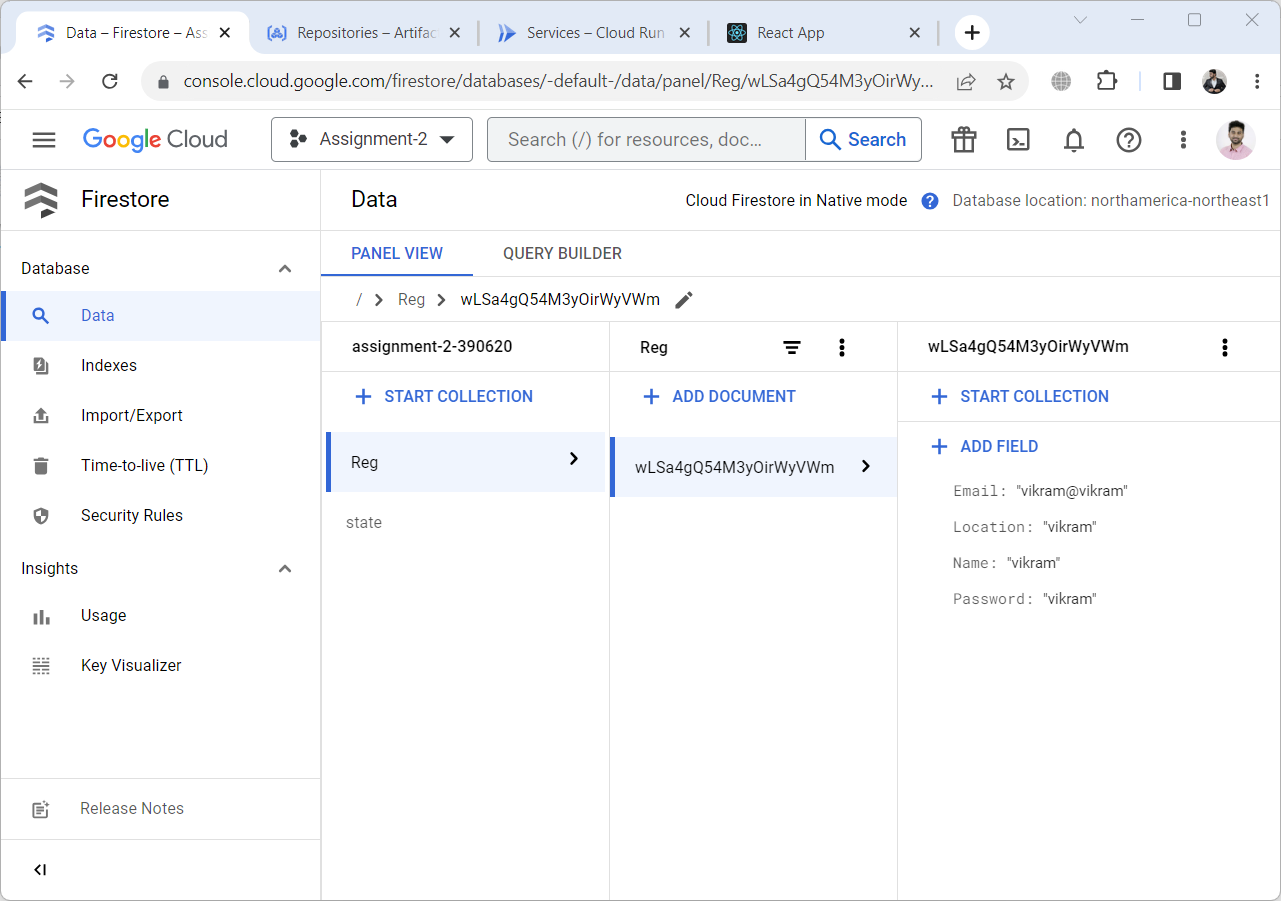
\includegraphics[scale=1, width=15cm,height=7.5cm]{PROBLEM 2/Screenshots/2. Demo/1.3 Vikram-record created.png}}
    \caption{\textbf{\textit{ User - Vikram: Document created in "Reg" }}}
    \label{fig:vikram-record-created}
\end{figure}


\begin{figure}[htp]
    \centering
    \fbox{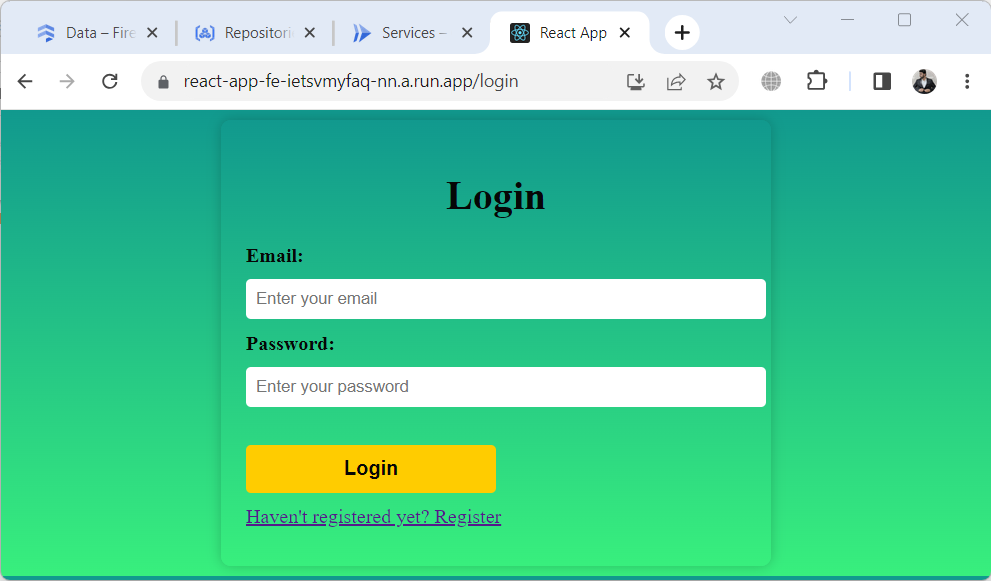
\includegraphics[scale=1, width=15cm,height=7.5cm]{PROBLEM 2/Screenshots/2. Demo/2. Login page.png}}
    \caption{\textbf{\textit{ Login page }}}
    \label{fig:login-page}
\end{figure}

\begin{figure}[htp]
    \centering
    \fbox{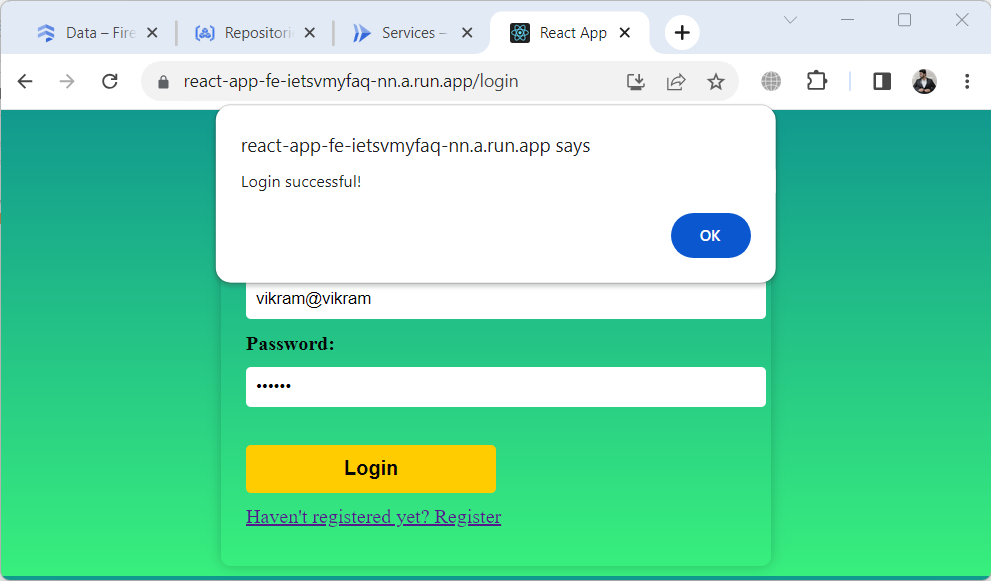
\includegraphics[scale=1, width=15cm,height=7.5cm]{PROBLEM 2/Screenshots/2. Demo/2.1 Login success.png}}
    \caption{\textbf{\textit{ User - Vikram: Login Success }}}
    \label{fig:vikram-login-success}
\end{figure}

\begin{figure}[htp]
    \centering
    \fbox{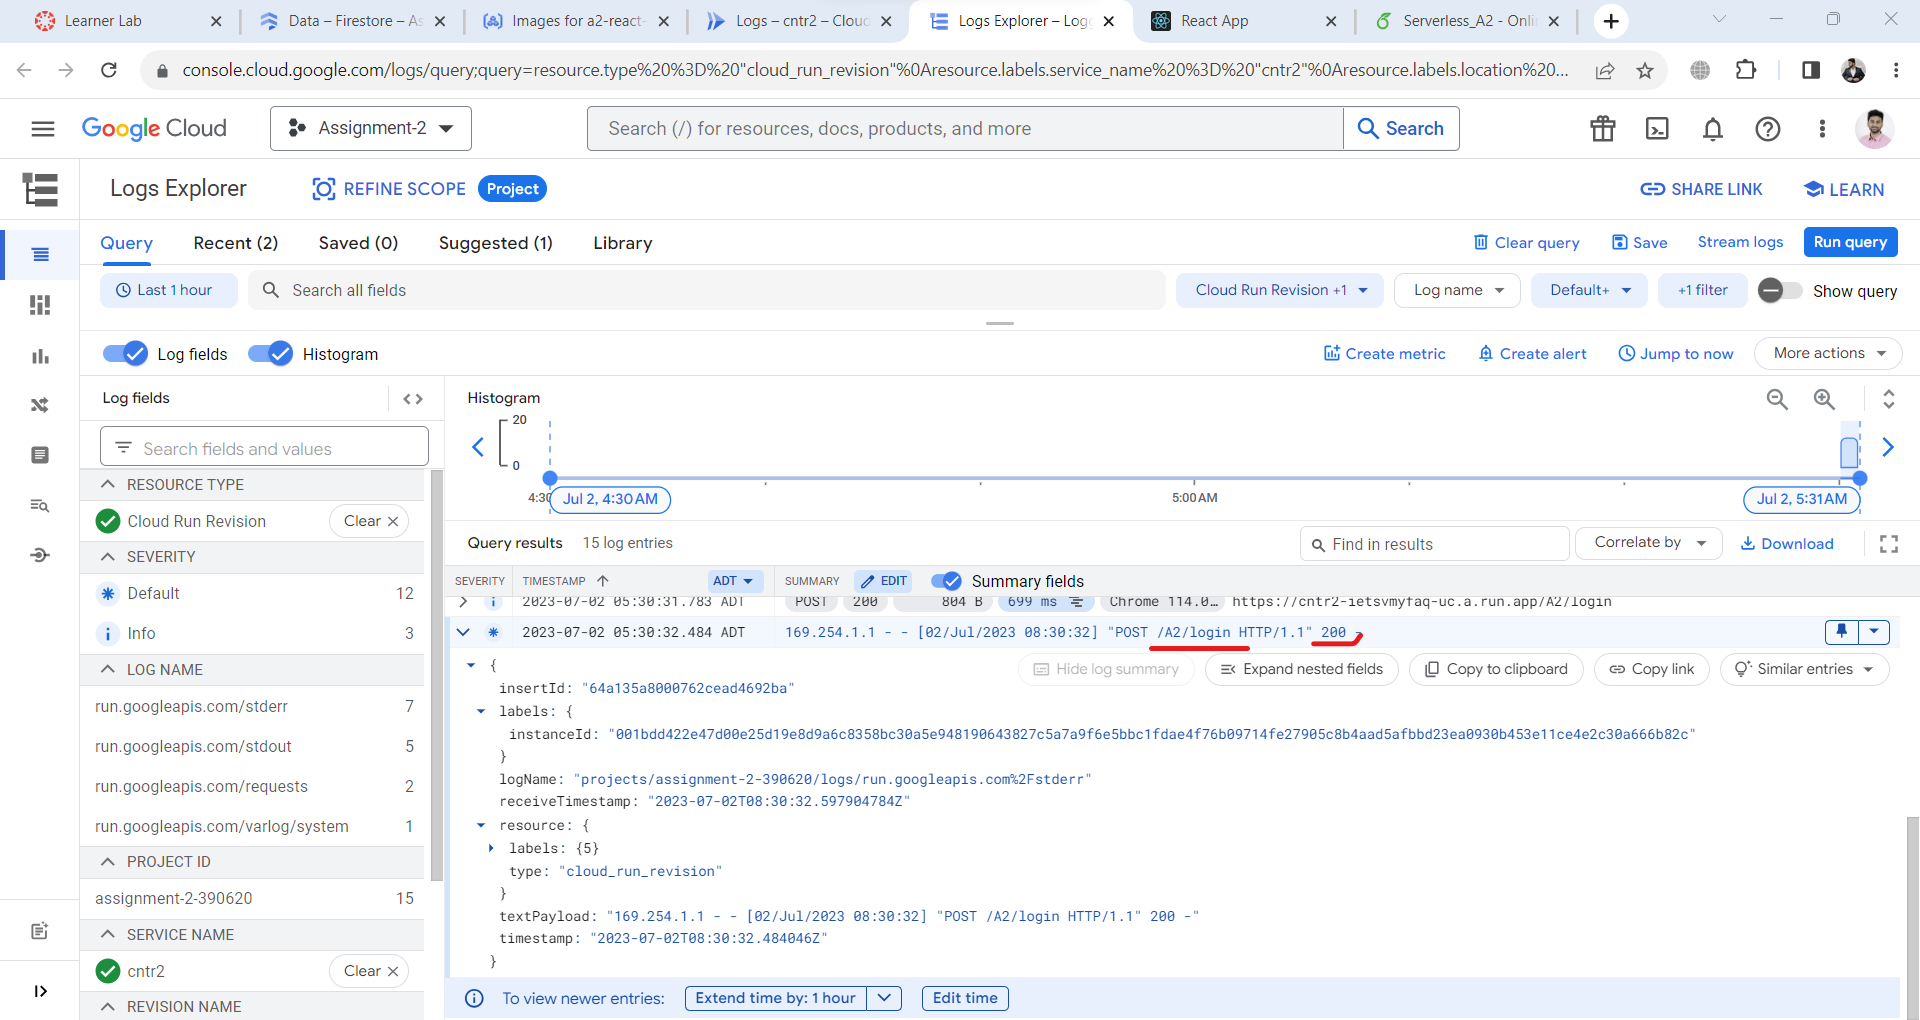
\includegraphics[scale=1, width=15cm,height=7.5cm]{PROBLEM 2/Screenshots/2. Demo/1. Logs/2. login success 200.png}}
    \caption{\textbf{\textit{ User - Vikram: Login logs }}}
    \label{fig:vikram-session-data-page}
\end{figure}

\begin{figure}[htp]
    \centering
    \fbox{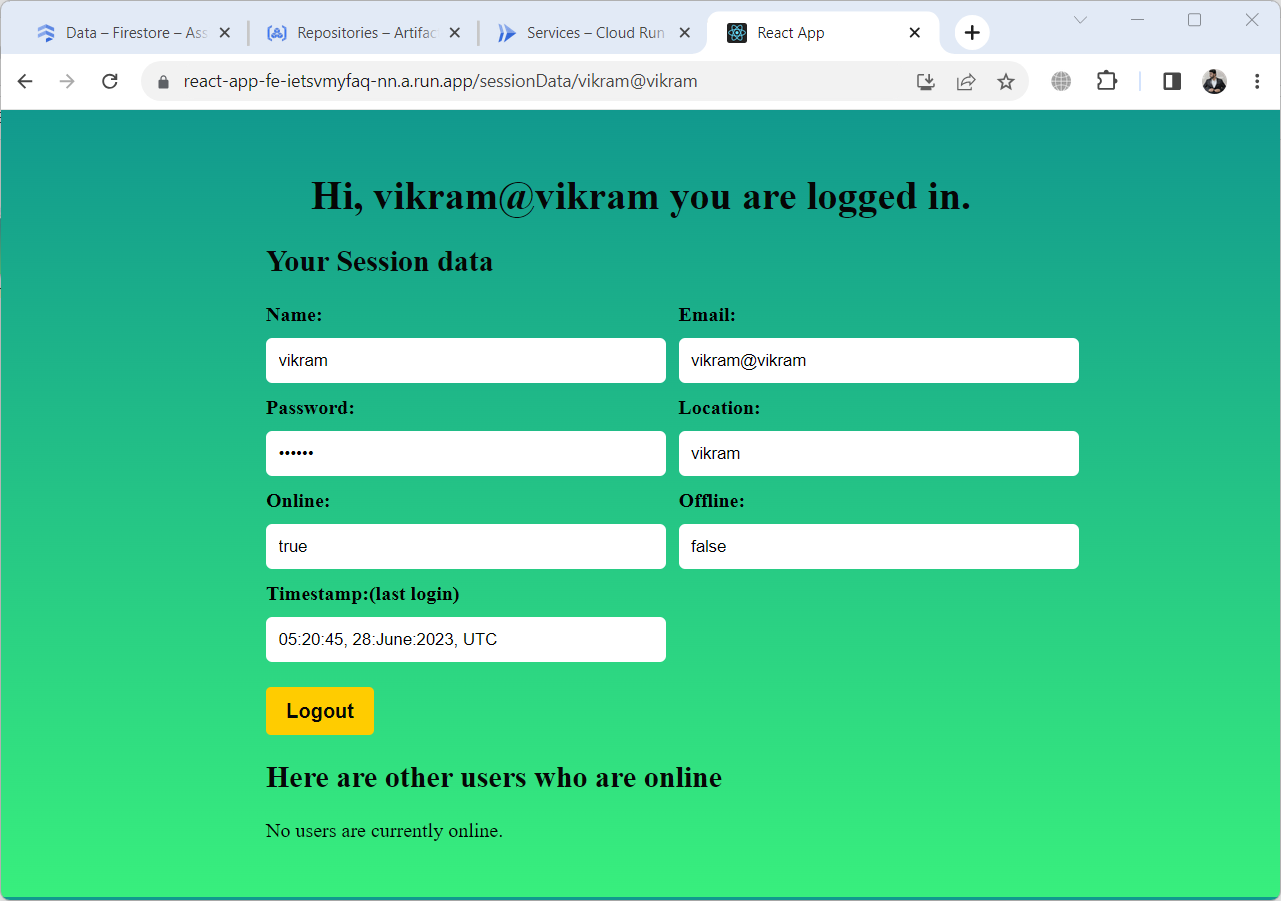
\includegraphics[scale=1, width=15cm,height=7.5cm]{PROBLEM 2/Screenshots/2. Demo/3.1 Session data for vikram.png}}
    \caption{\textbf{\textit{ User - Vikram: Session data page (no other users online) }}}
    \label{fig:vikram-session-data-page}
\end{figure}

\begin{figure}[htp]
    \centering
    \fbox{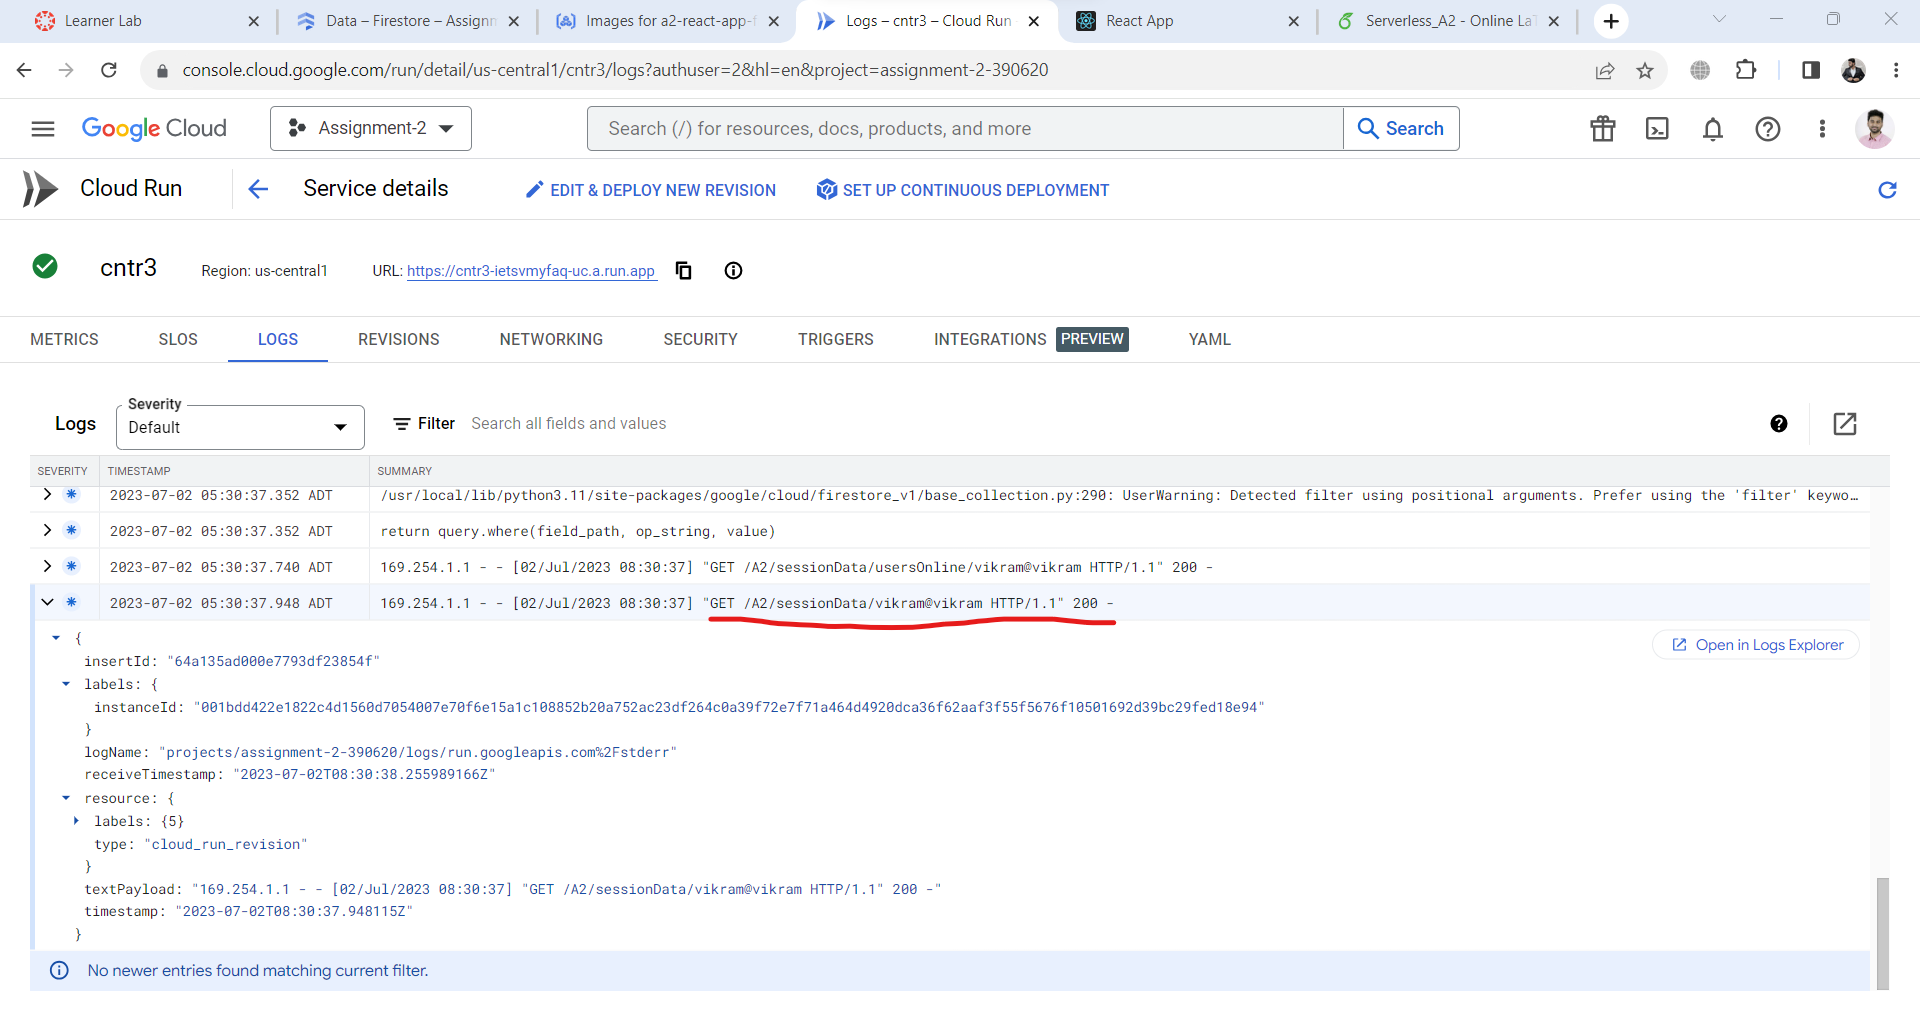
\includegraphics[scale=1, width=15cm,height=7.5cm]{PROBLEM 2/Screenshots/2. Demo/1. Logs/3. session vikram showing.png}}
    \caption{\textbf{\textit{ User - Vikram: session logs }}}
    \label{fig:vikram-session-data-page}
\end{figure}

\begin{figure}[htp]
    \centering
    \fbox{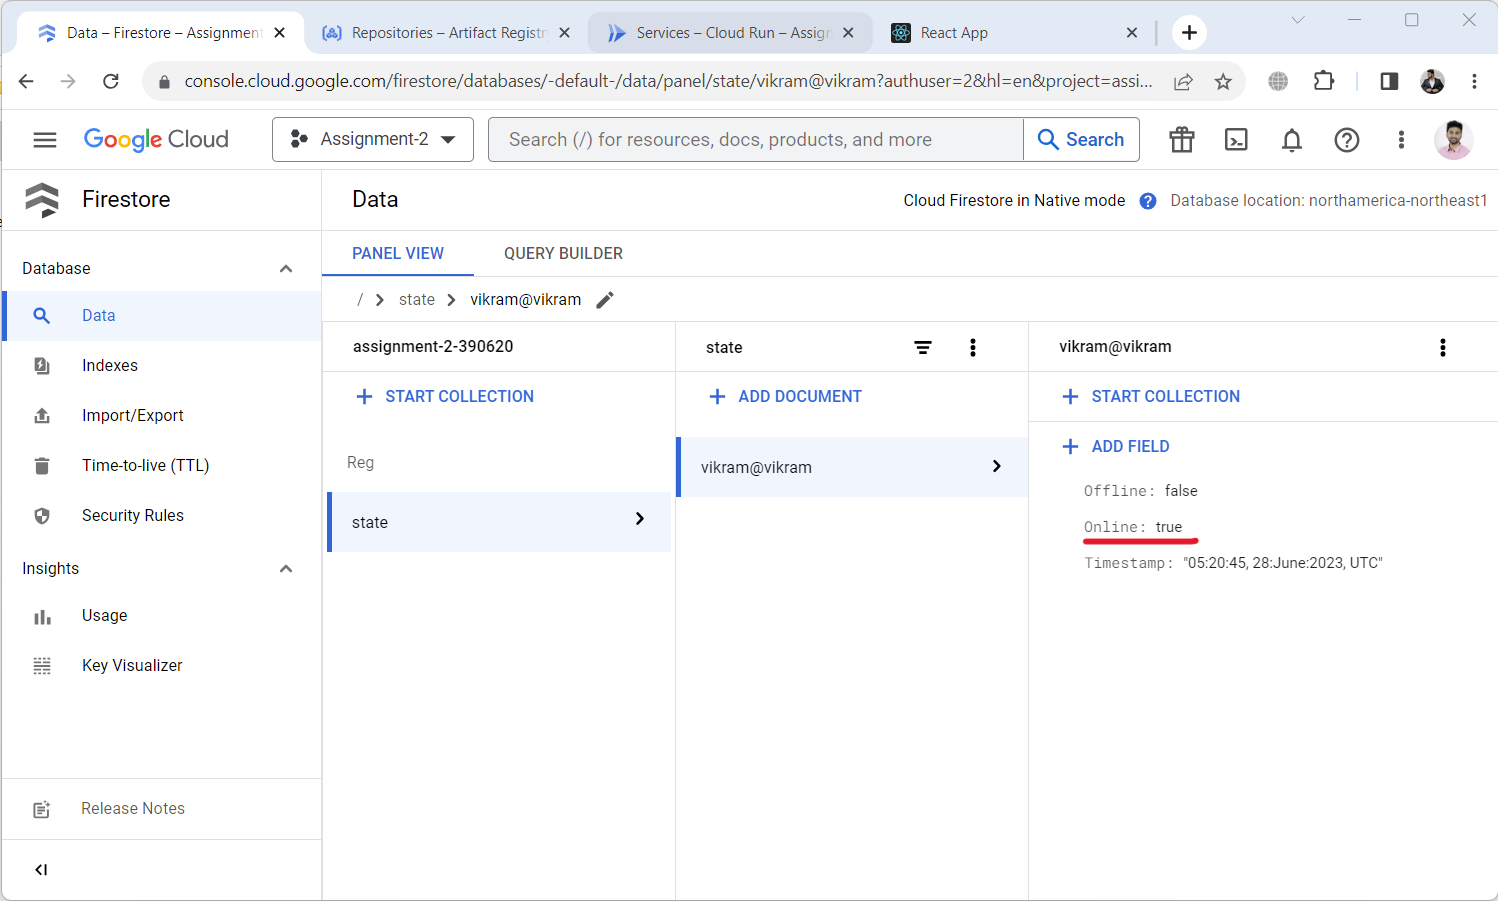
\includegraphics[scale=1, width=15cm,height=7.5cm]{PROBLEM 2/Screenshots/2. Demo/3.2 vikram - after login - online.png}}
    \caption{\textbf{\textit{ User - Vikram: Session data document in "state"}}}
    \label{fig:vikram-session-data-document}
\end{figure}

\begin{figure}[htp]
    \centering
    \fbox{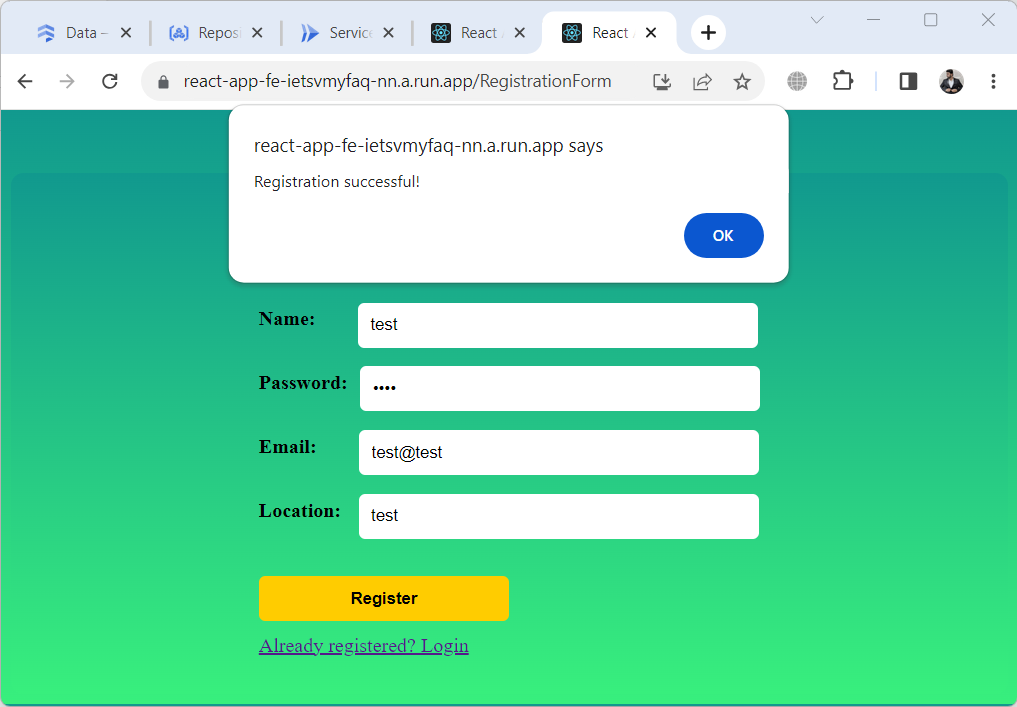
\includegraphics[scale=1, width=15cm,height=7.5cm]{PROBLEM 2/Screenshots/2. Demo/4.1 test- reg success.png}}
    \caption{\textbf{\textit{ User - test: Registration success}}}
    \label{fig:test-reg-success}
\end{figure}

\begin{figure}[htp]
    \centering
    \fbox{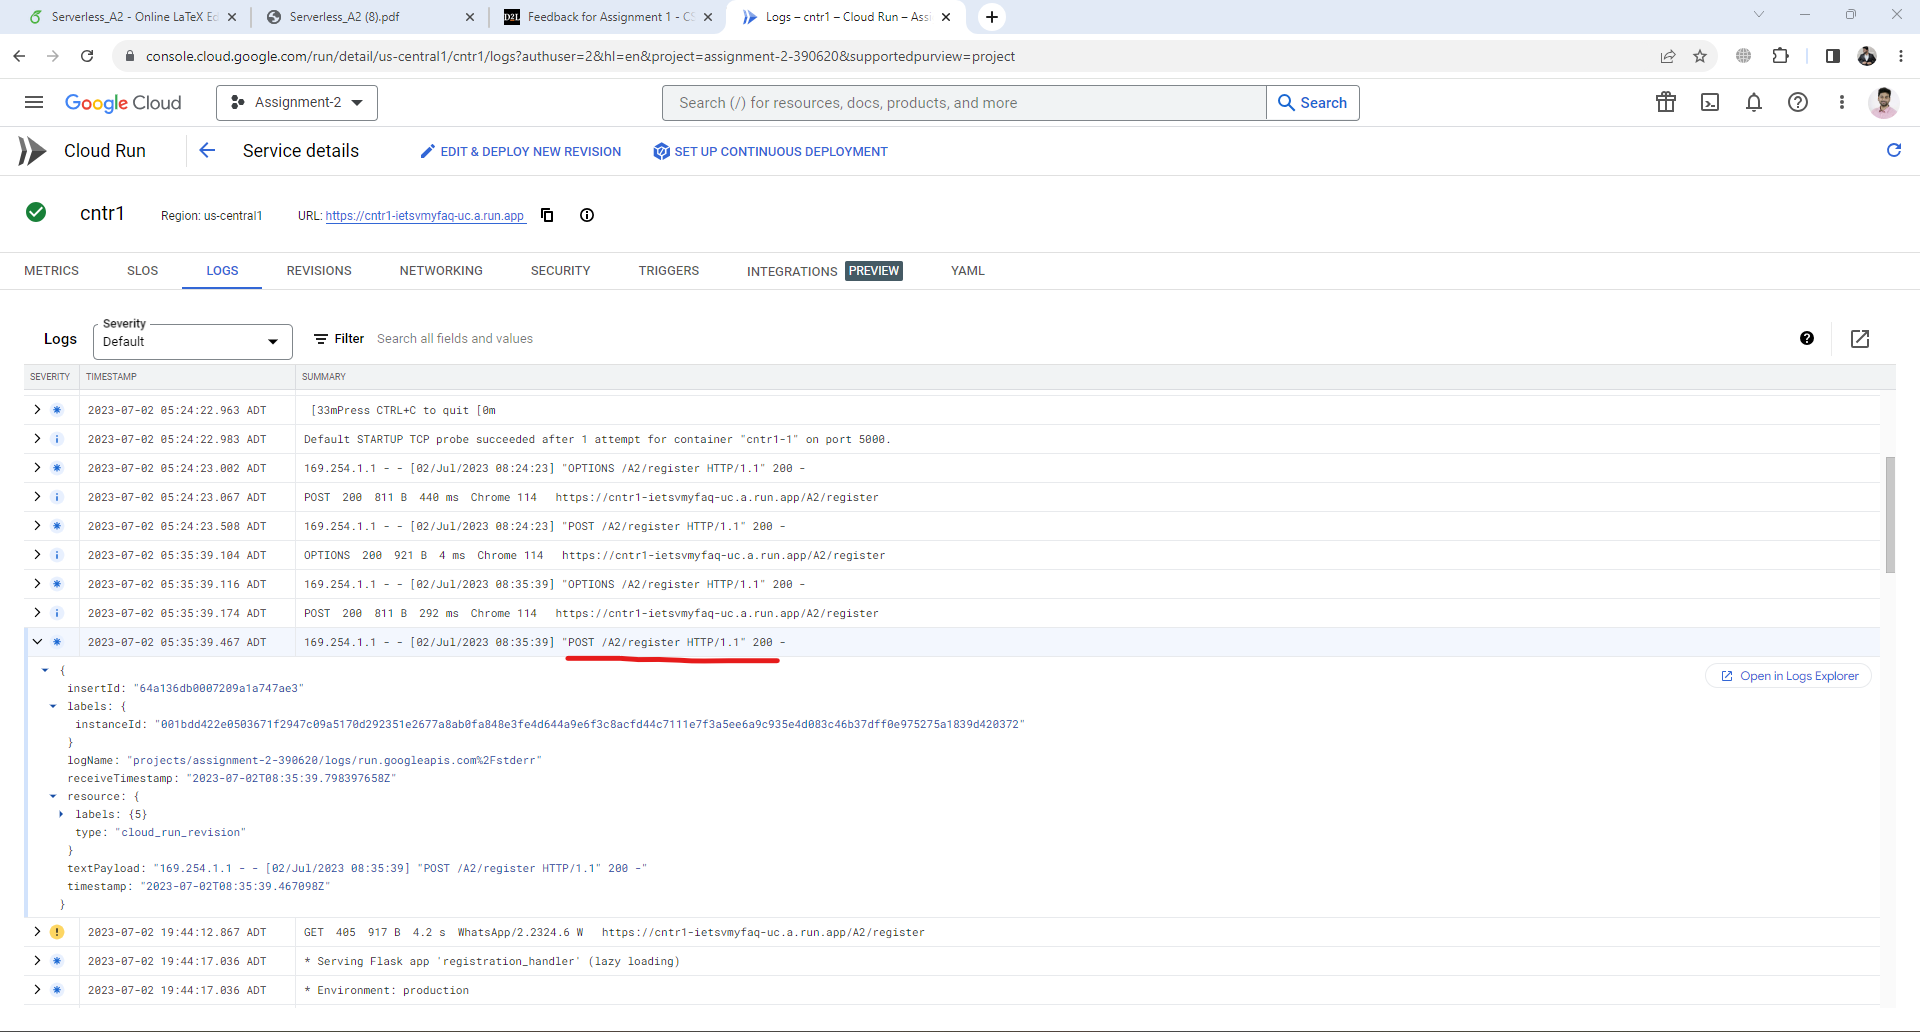
\includegraphics[scale=1, width=15cm,height=7.5cm]{PROBLEM 2/Screenshots/2. Demo/1. Logs/1.1 test reg success.png}}
    \caption{\textbf{\textit{ User - test: Registration success logs}}}
    \label{fig:test-reg-success}
\end{figure}

\begin{figure}[htp]
    \centering
    \fbox{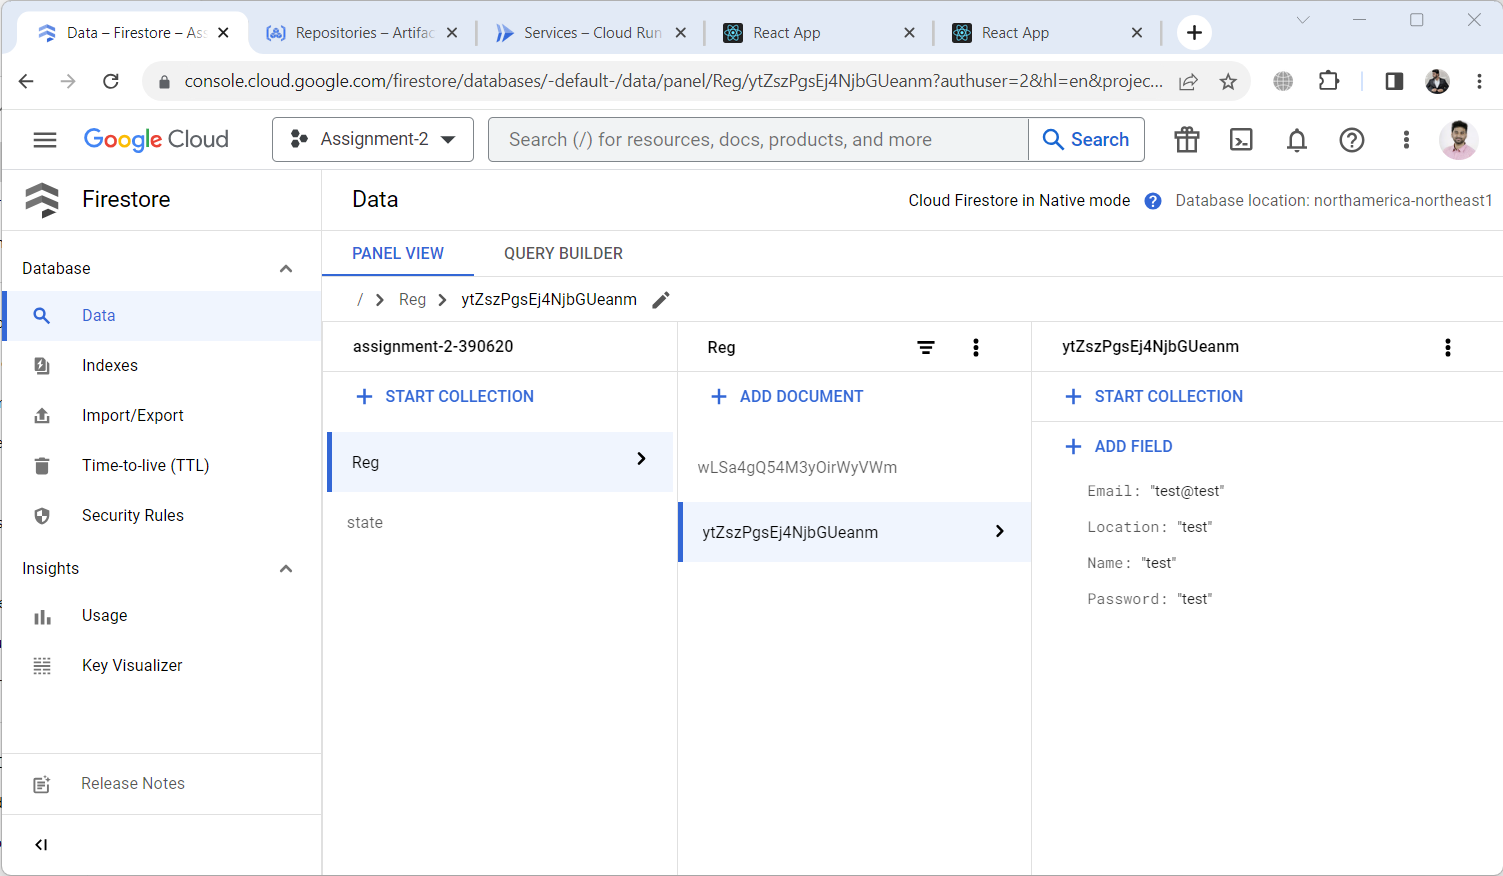
\includegraphics[scale=1, width=15cm,height=7.5cm]{PROBLEM 2/Screenshots/2. Demo/4.2 test record created in Reg.png}}
    \caption{\textbf{\textit{ User - test: document created in "Reg"}}}
    \label{fig:test-record-created-reg}
\end{figure}

\begin{figure}[htp]
    \centering
    \fbox{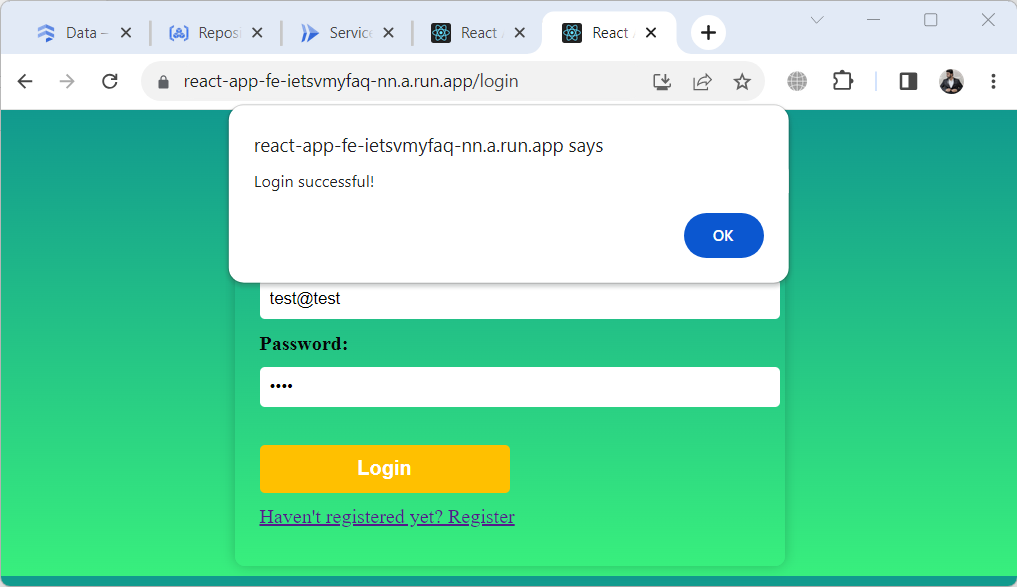
\includegraphics[scale=1, width=15cm,height=7.5cm]{PROBLEM 2/Screenshots/2. Demo/4.3 test- login success.png}}
    \caption{\textbf{\textit{ User - test: Login success }}}
    \label{fig:test-login-success}
\end{figure}

\begin{figure}[htp]
    \centering
    \fbox{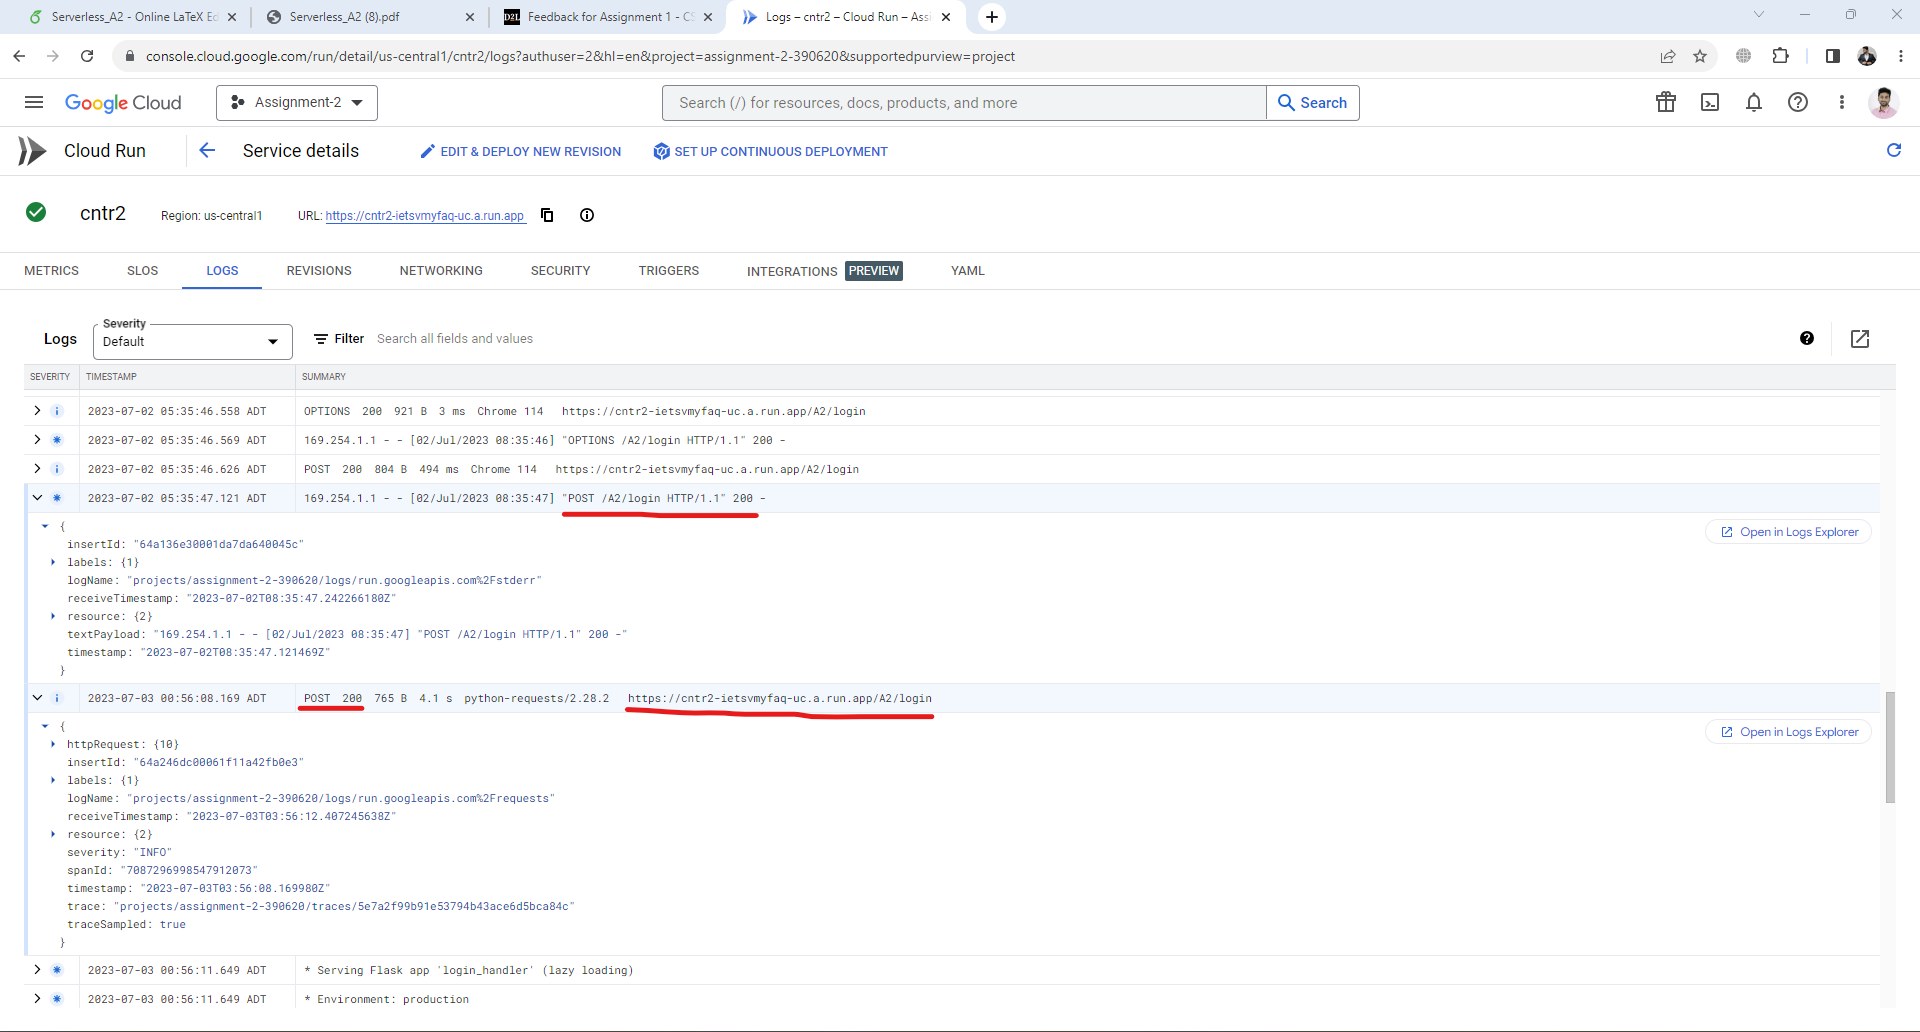
\includegraphics[scale=1, width=15cm,height=7.5cm]{PROBLEM 2/Screenshots/2. Demo/1. Logs/2.2 test login success.png}}
    \caption{\textbf{\textit{ User - test: Login success logs}}}
    \label{fig:test-login-success}
\end{figure}

\begin{figure}[htp]
    \centering
    \fbox{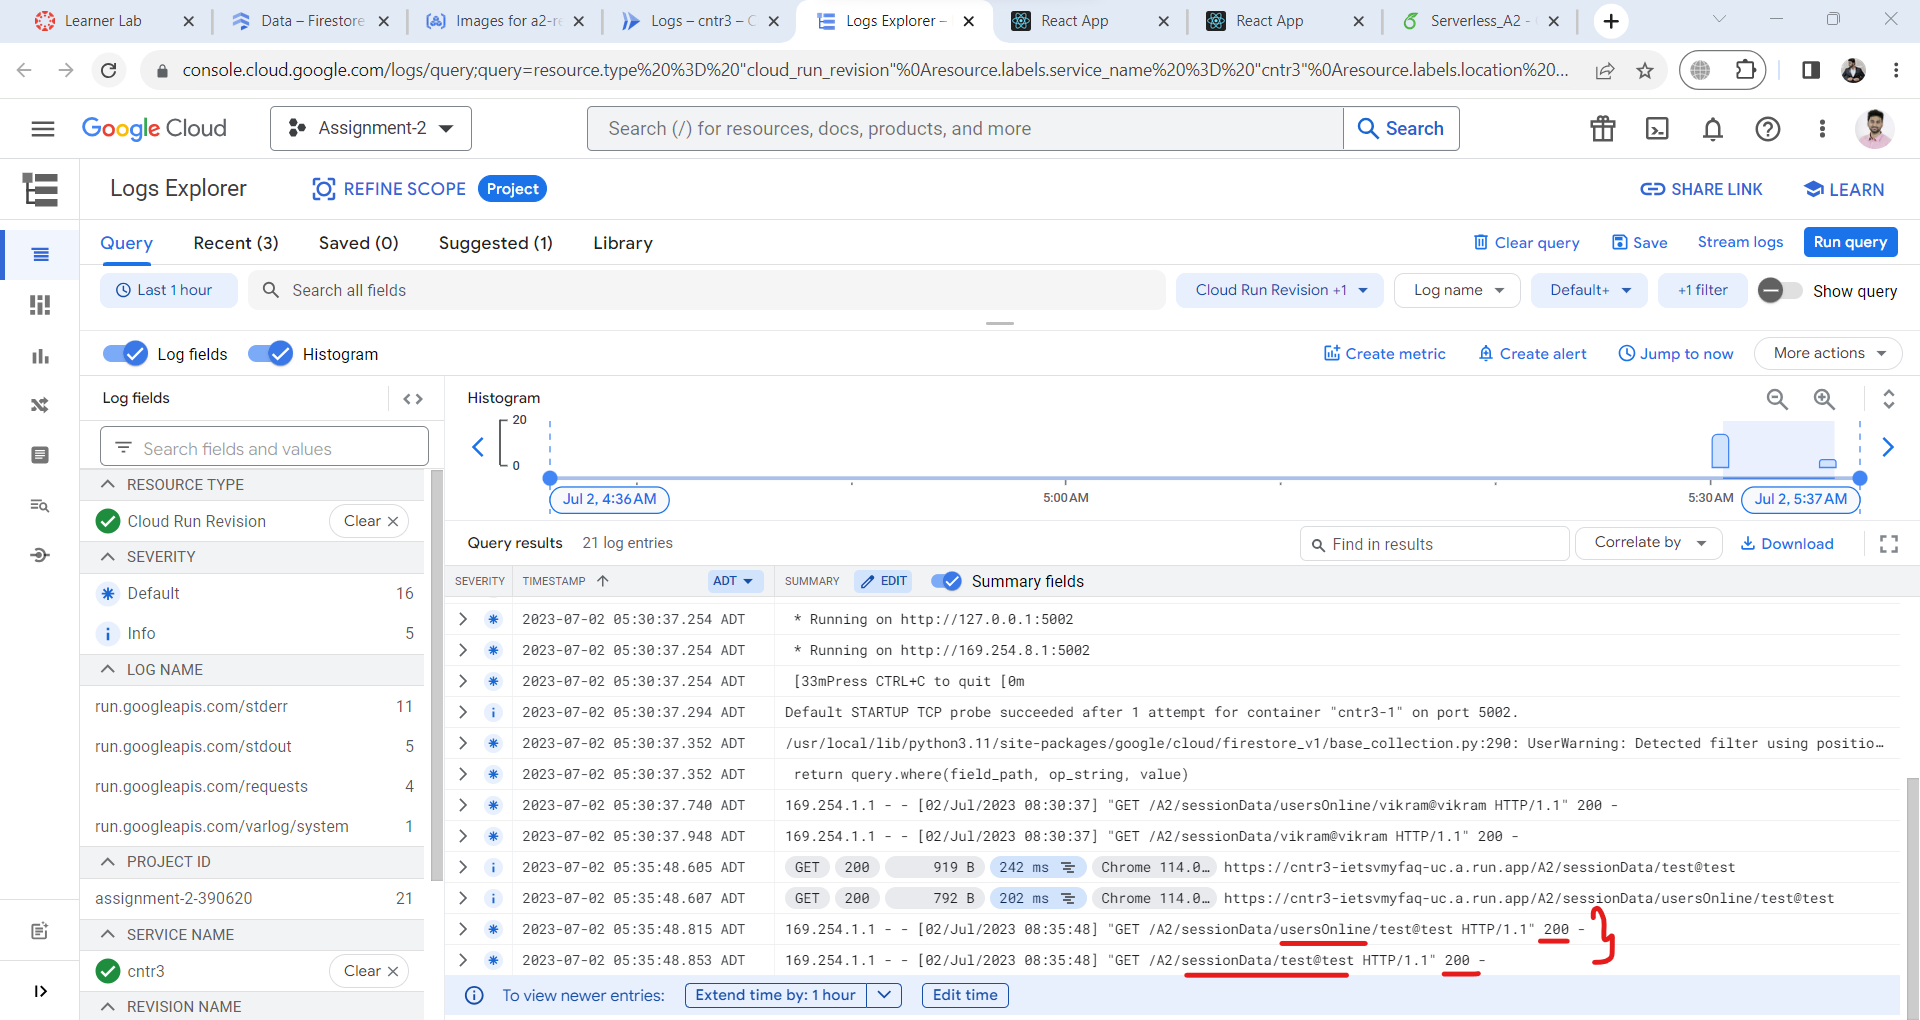
\includegraphics[scale=1, width=15cm,height=7.5cm]{PROBLEM 2/Screenshots/2. Demo/1. Logs/3. session test showing .png}}
    \caption{\textbf{\textit{ User - test: Session data logs }}}
    \label{fig:test-login-success}
\end{figure}

\begin{figure}[htp]
    \centering
    \fbox{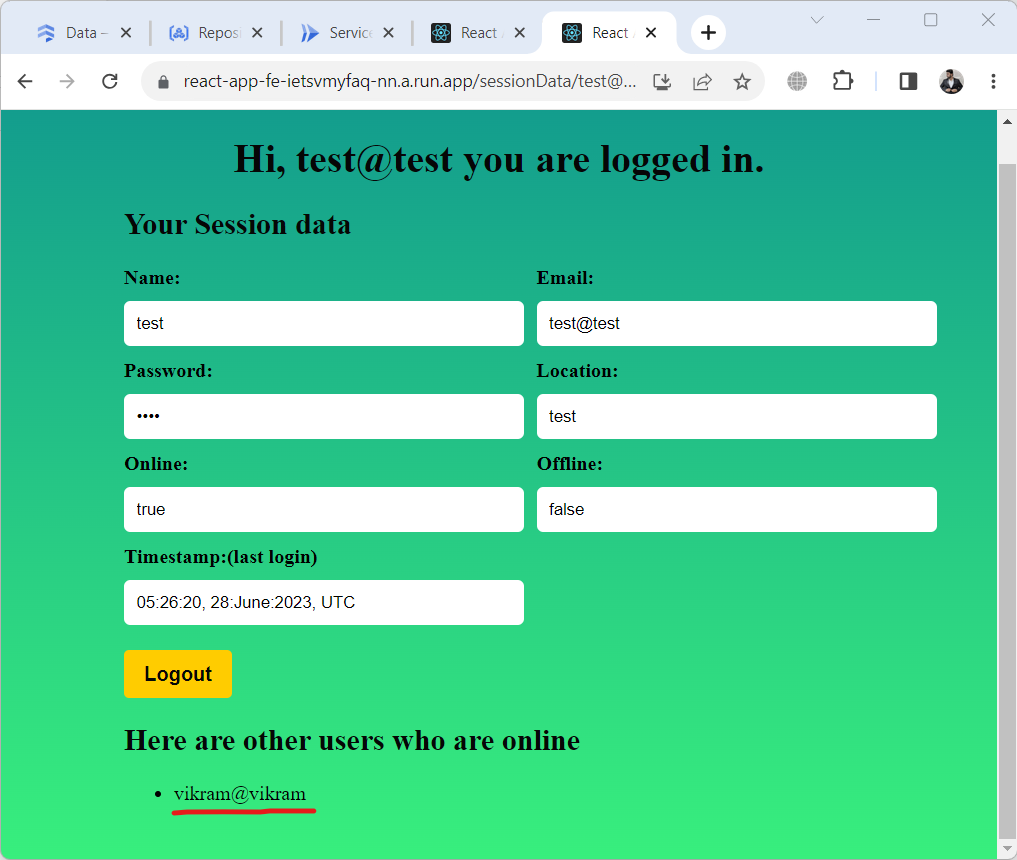
\includegraphics[scale=1, width=15cm,height=7.5cm]{PROBLEM 2/Screenshots/2. Demo/5.1 test session data - vikram online displaying.png}}
    \caption{\textbf{\textit{ User - test: session data (other online user(s) - "Vikram" is displaying) }}}
    \label{fig:test-session-data}
\end{figure}

\begin{figure}[htp]
    \centering
    \fbox{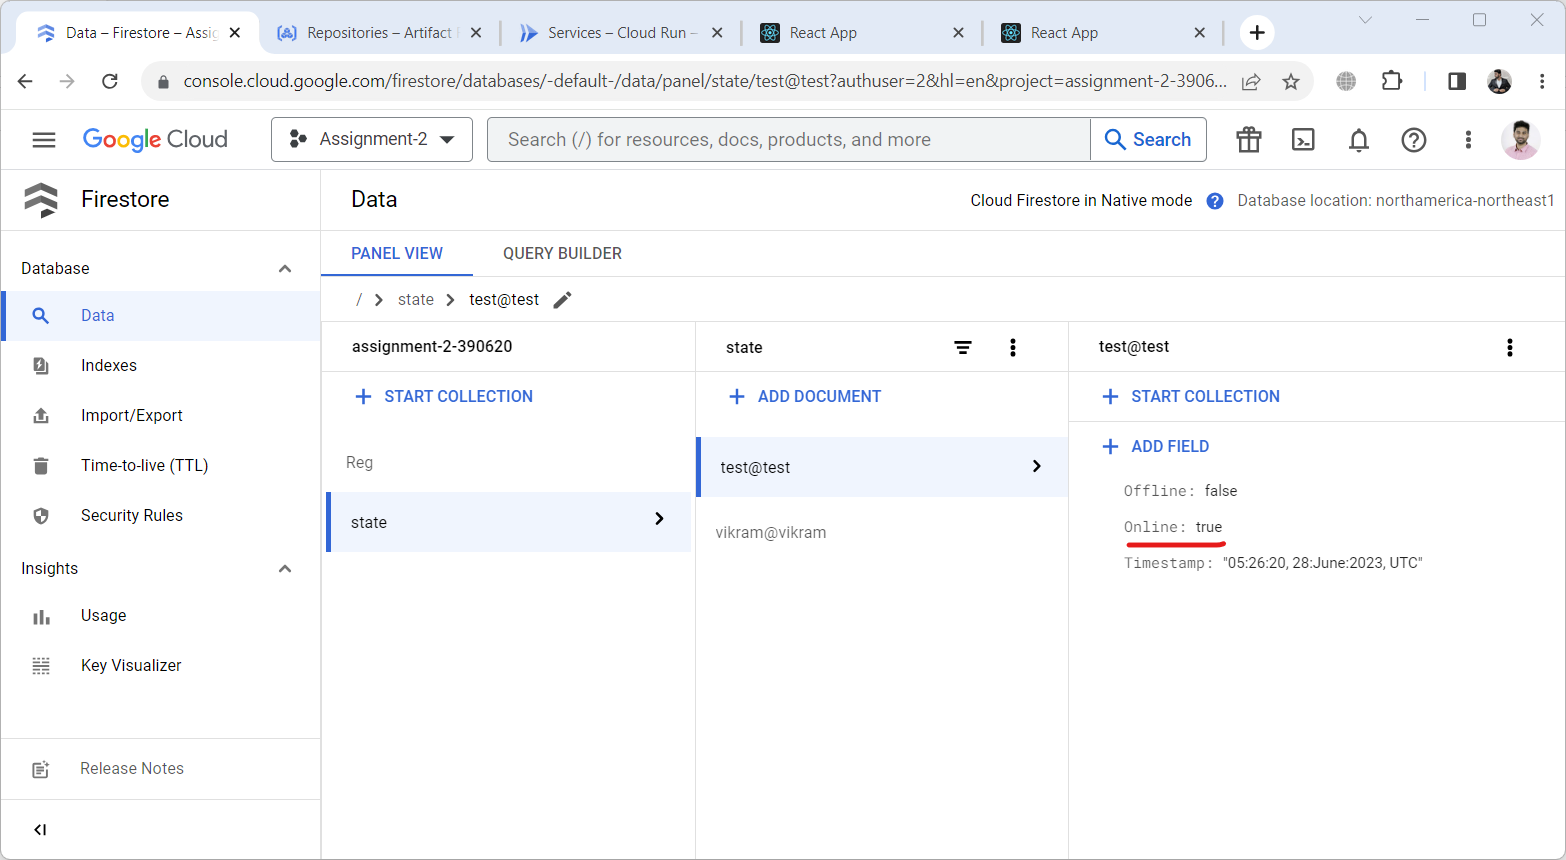
\includegraphics[scale=1, width=15cm,height=7.5cm]{PROBLEM 2/Screenshots/2. Demo/4.4 test after login - online.png}}
    \caption{\textbf{\textit{ User - test: document created in "state" }}}
    \label{fig:test-record-created-state}
\end{figure}



\begin{figure}[htp]
    \centering
    \fbox{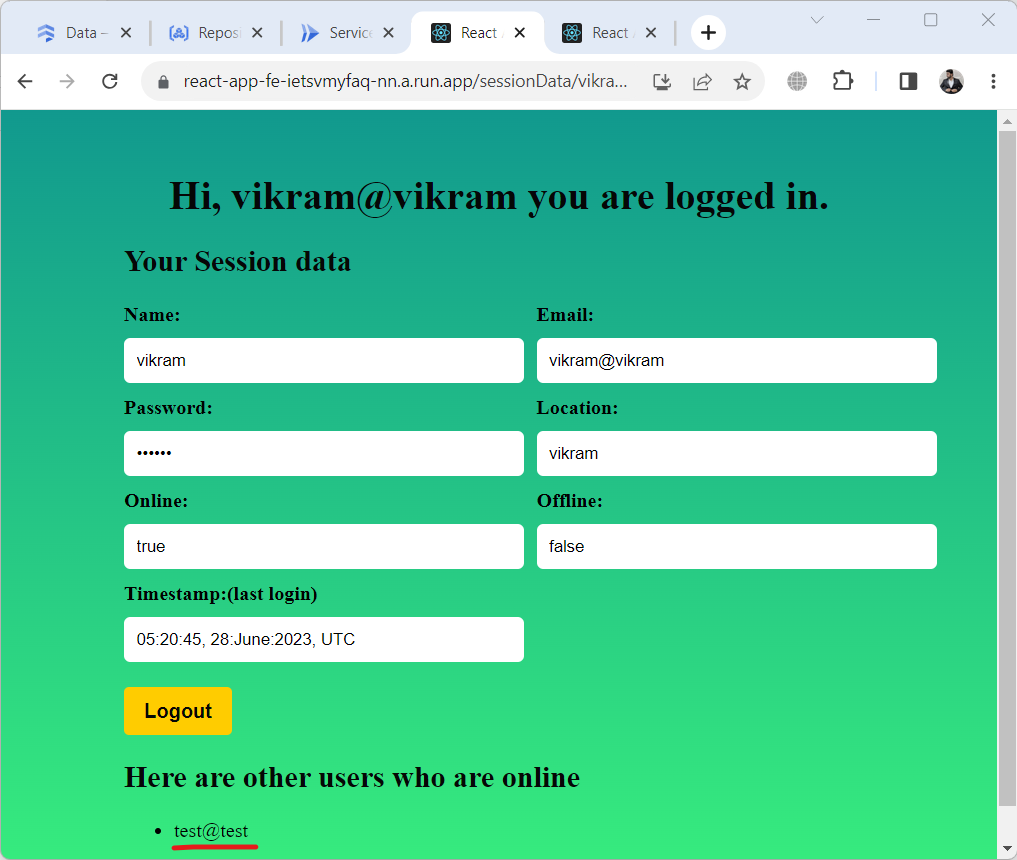
\includegraphics[scale=1, width=15cm,height=7.5cm]{PROBLEM 2/Screenshots/2. Demo/5.2 vikram session - test online displaying after refresh.png}}
    \caption{\textbf{\textit{ User - Vikram: session data (other online user(s) - "test" is displaying after refreshing the page) }}}
    \label{fig:vikram-session-data-refresh}
\end{figure}

\begin{figure}[htp]
    \centering
    \fbox{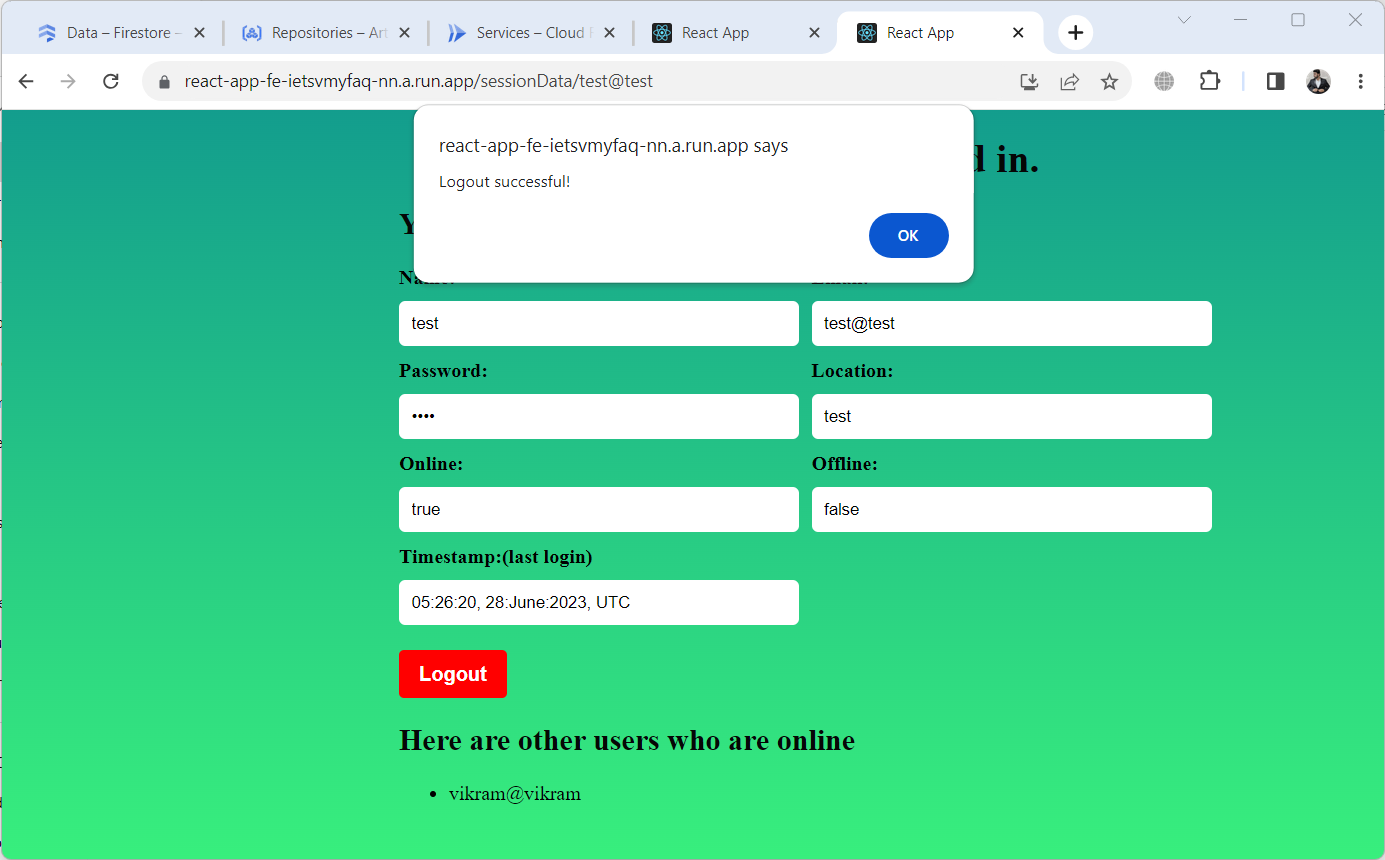
\includegraphics[scale=1, width=15cm,height=7.5cm]{PROBLEM 2/Screenshots/2. Demo/6.1 test - logout success.png}}
    \caption{\textbf{\textit{ User - test: Logout success }}}
    \label{fig:test-logout-success}
\end{figure}

\begin{figure}[htp]
    \centering
    \fbox{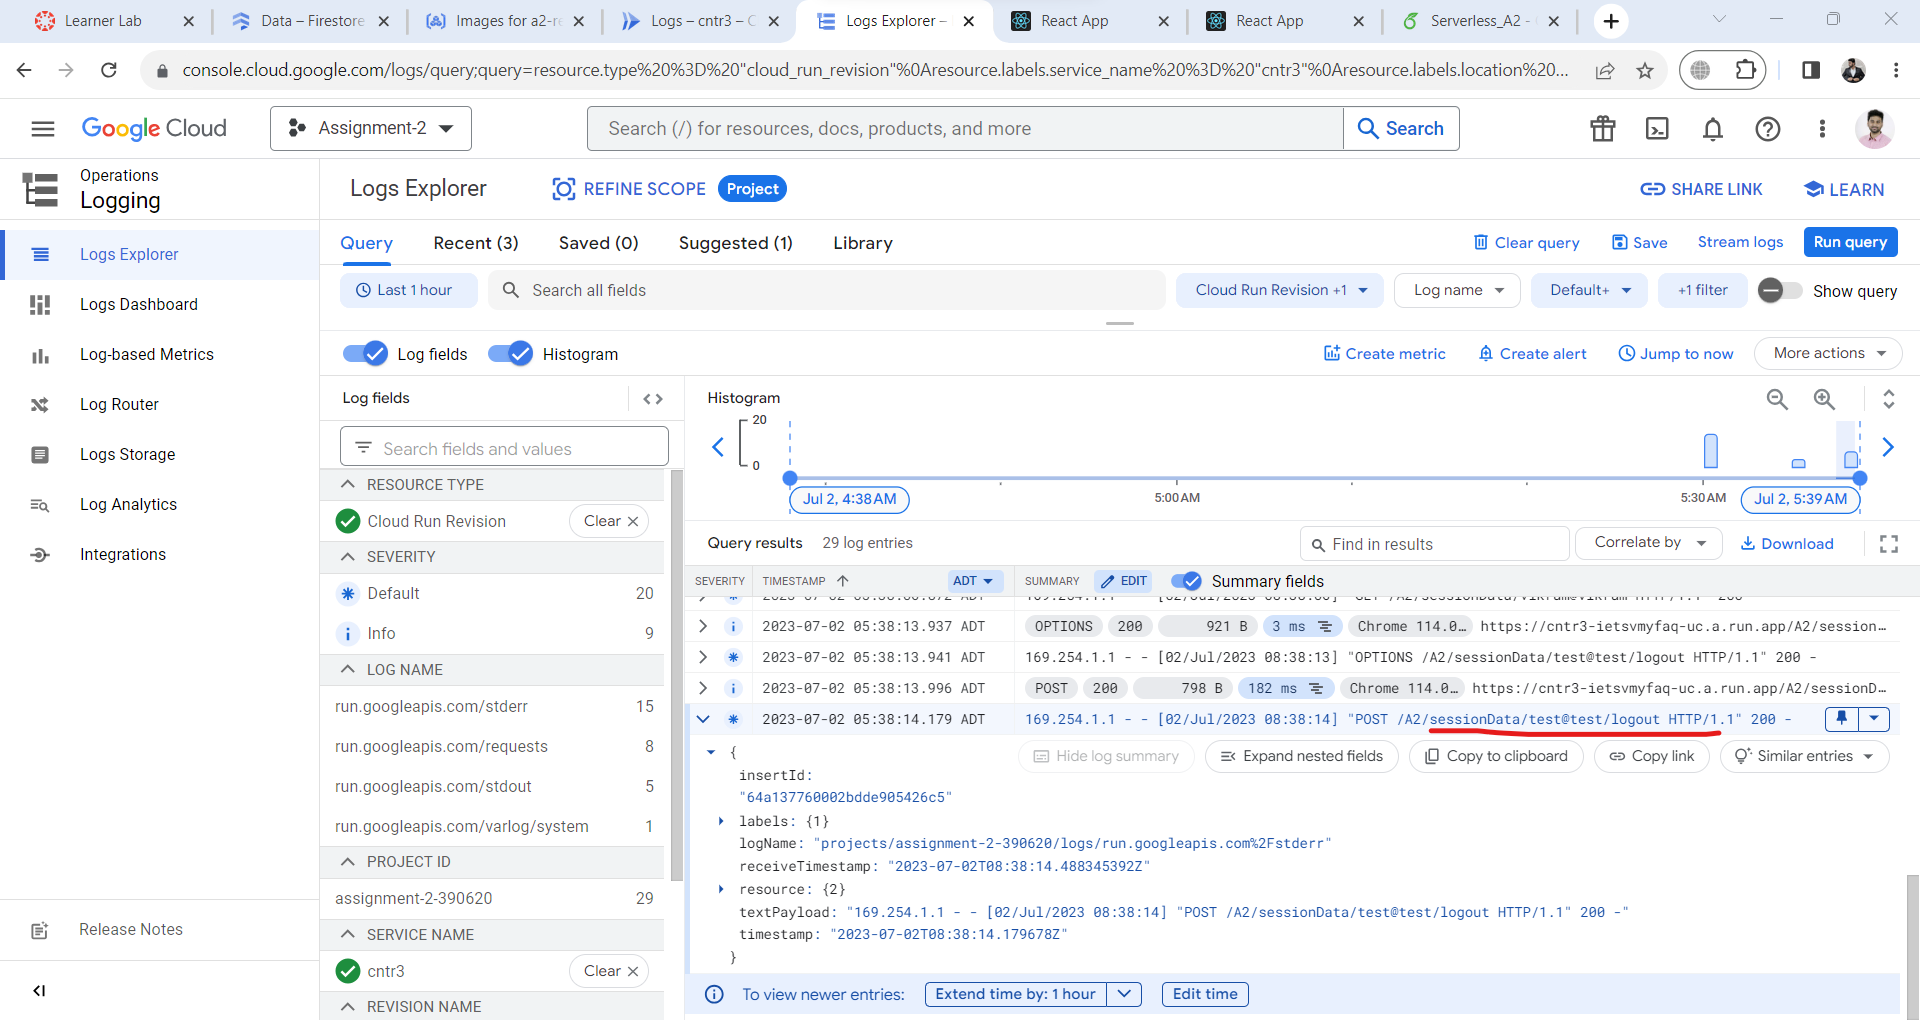
\includegraphics[scale=1, width=15cm,height=7.5cm]{PROBLEM 2/Screenshots/2. Demo/1. Logs/4. test session logout.png}}
    \caption{\textbf{\textit{ User - test: Logout logs }}}
    \label{fig:test-logout-success}
\end{figure}

\begin{figure}[htp]
    \centering
    \fbox{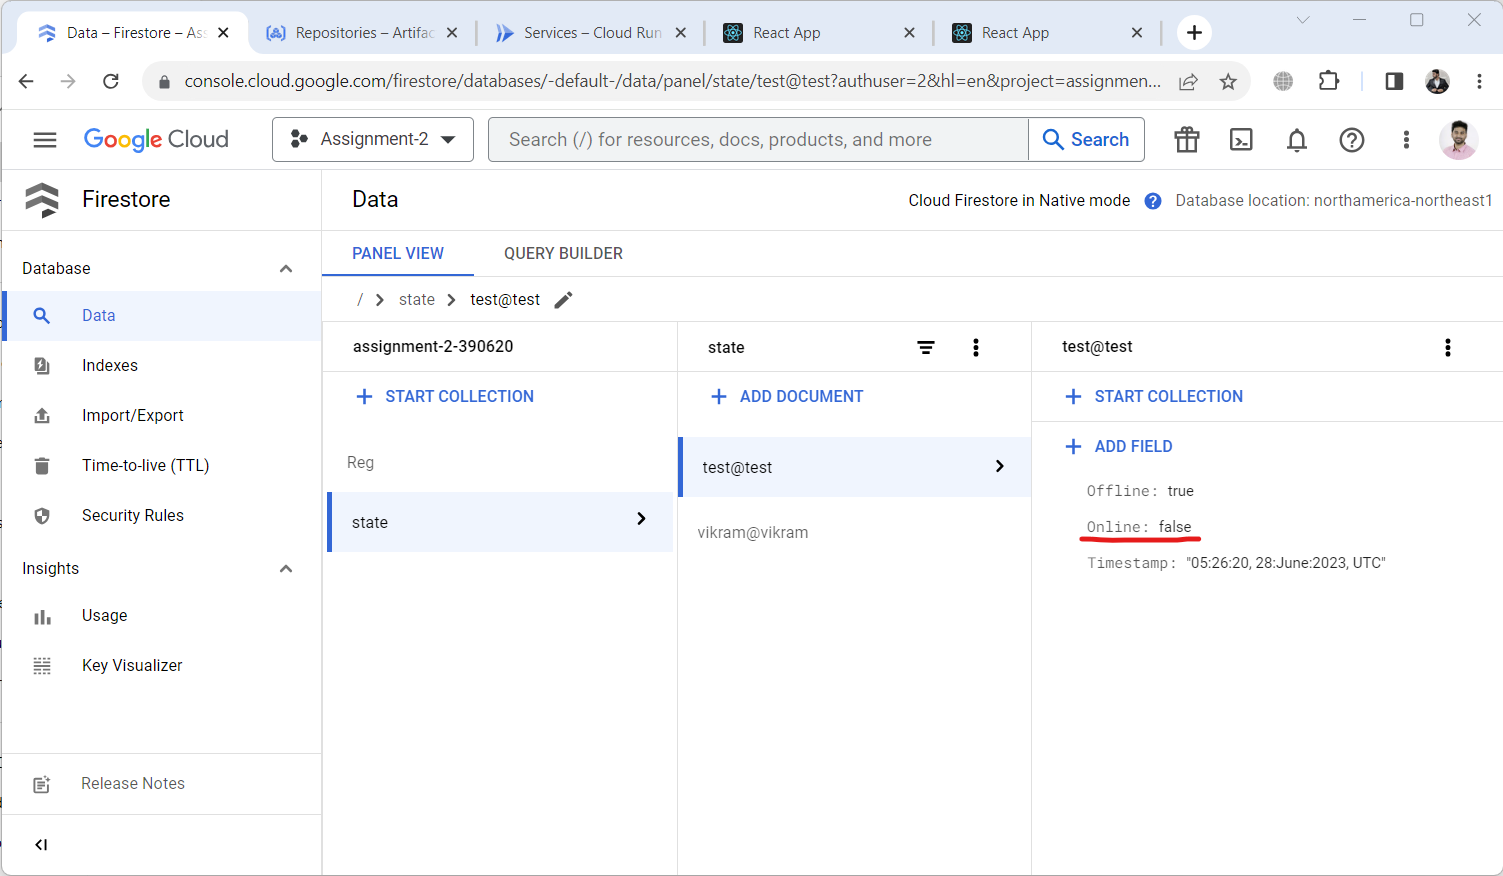
\includegraphics[scale=1, width=15cm,height=7.5cm]{PROBLEM 2/Screenshots/2. Demo/6.2 test session - offline after logout.png}}
    \caption{\textbf{\textit{ User - test: Session is Offline }}}
    \label{fig:test-session-offline}
\end{figure}

\begin{figure}[htp]
    \centering
    \fbox{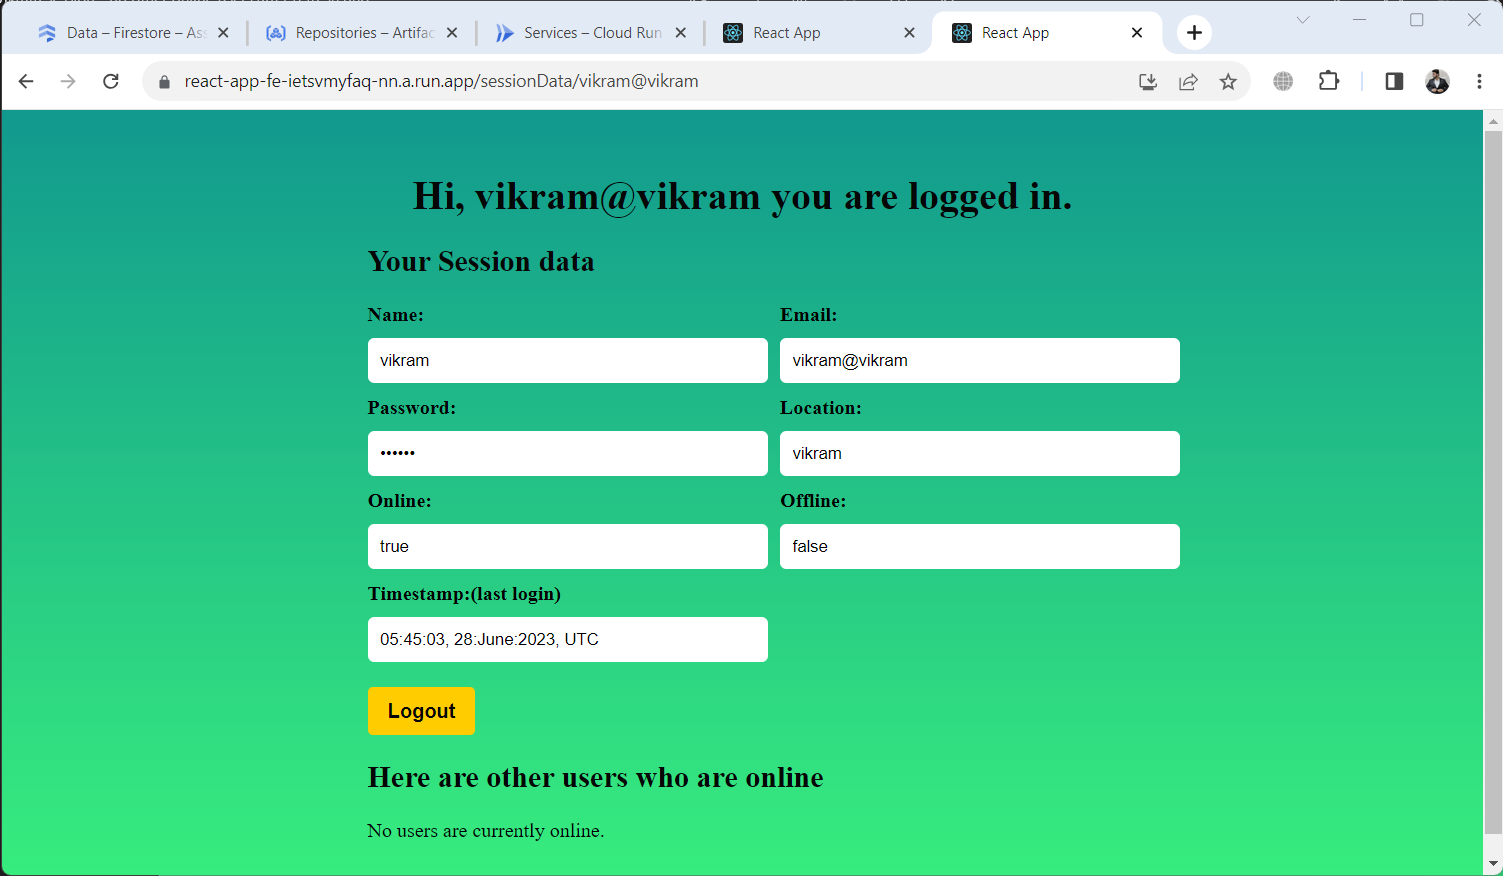
\includegraphics[scale=1, width=15cm,height=7.5cm]{PROBLEM 2/Screenshots/2. Demo/7.1 vikram session - no other online users after refresh.png}}
    \caption{\textbf{\textit{ User - Vikram: no users are online after user: test logged out (after refreshing the page) }}}
    \label{fig:vikram-session-after-test-logout}
\end{figure}

\begin{figure}[htp]
    \centering
    \fbox{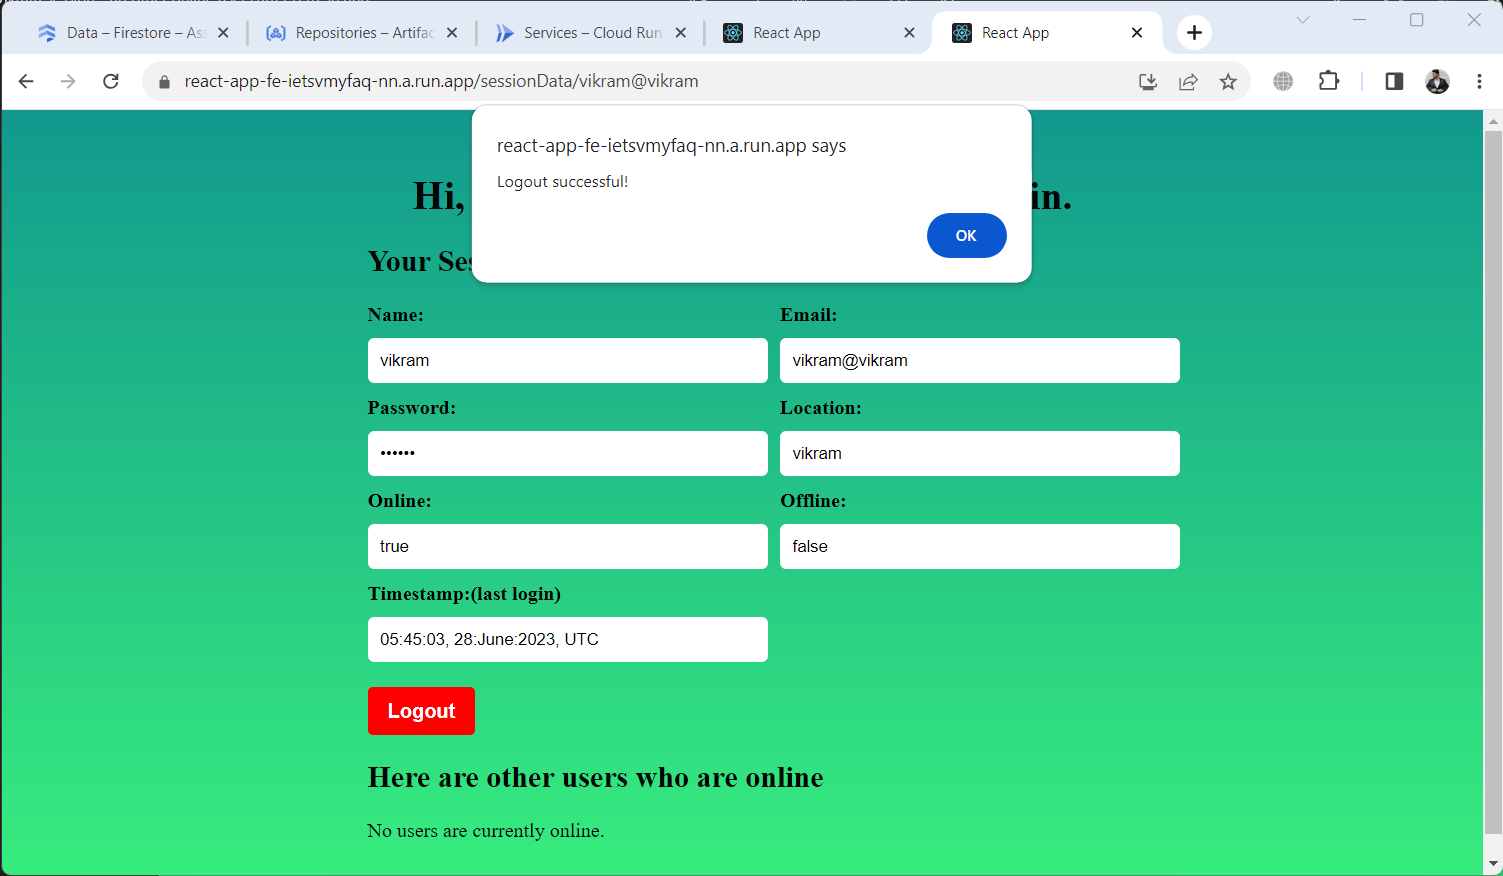
\includegraphics[scale=1, width=15cm,height=7.5cm]{PROBLEM 2/Screenshots/2. Demo/7.2 vikram - logout success.png}}
    \caption{\textbf{\textit{User - Vikram: Logout success}}}
    \label{fig:vikram-logout-success}
\end{figure}

\begin{figure}[htp]
    \centering
    \fbox{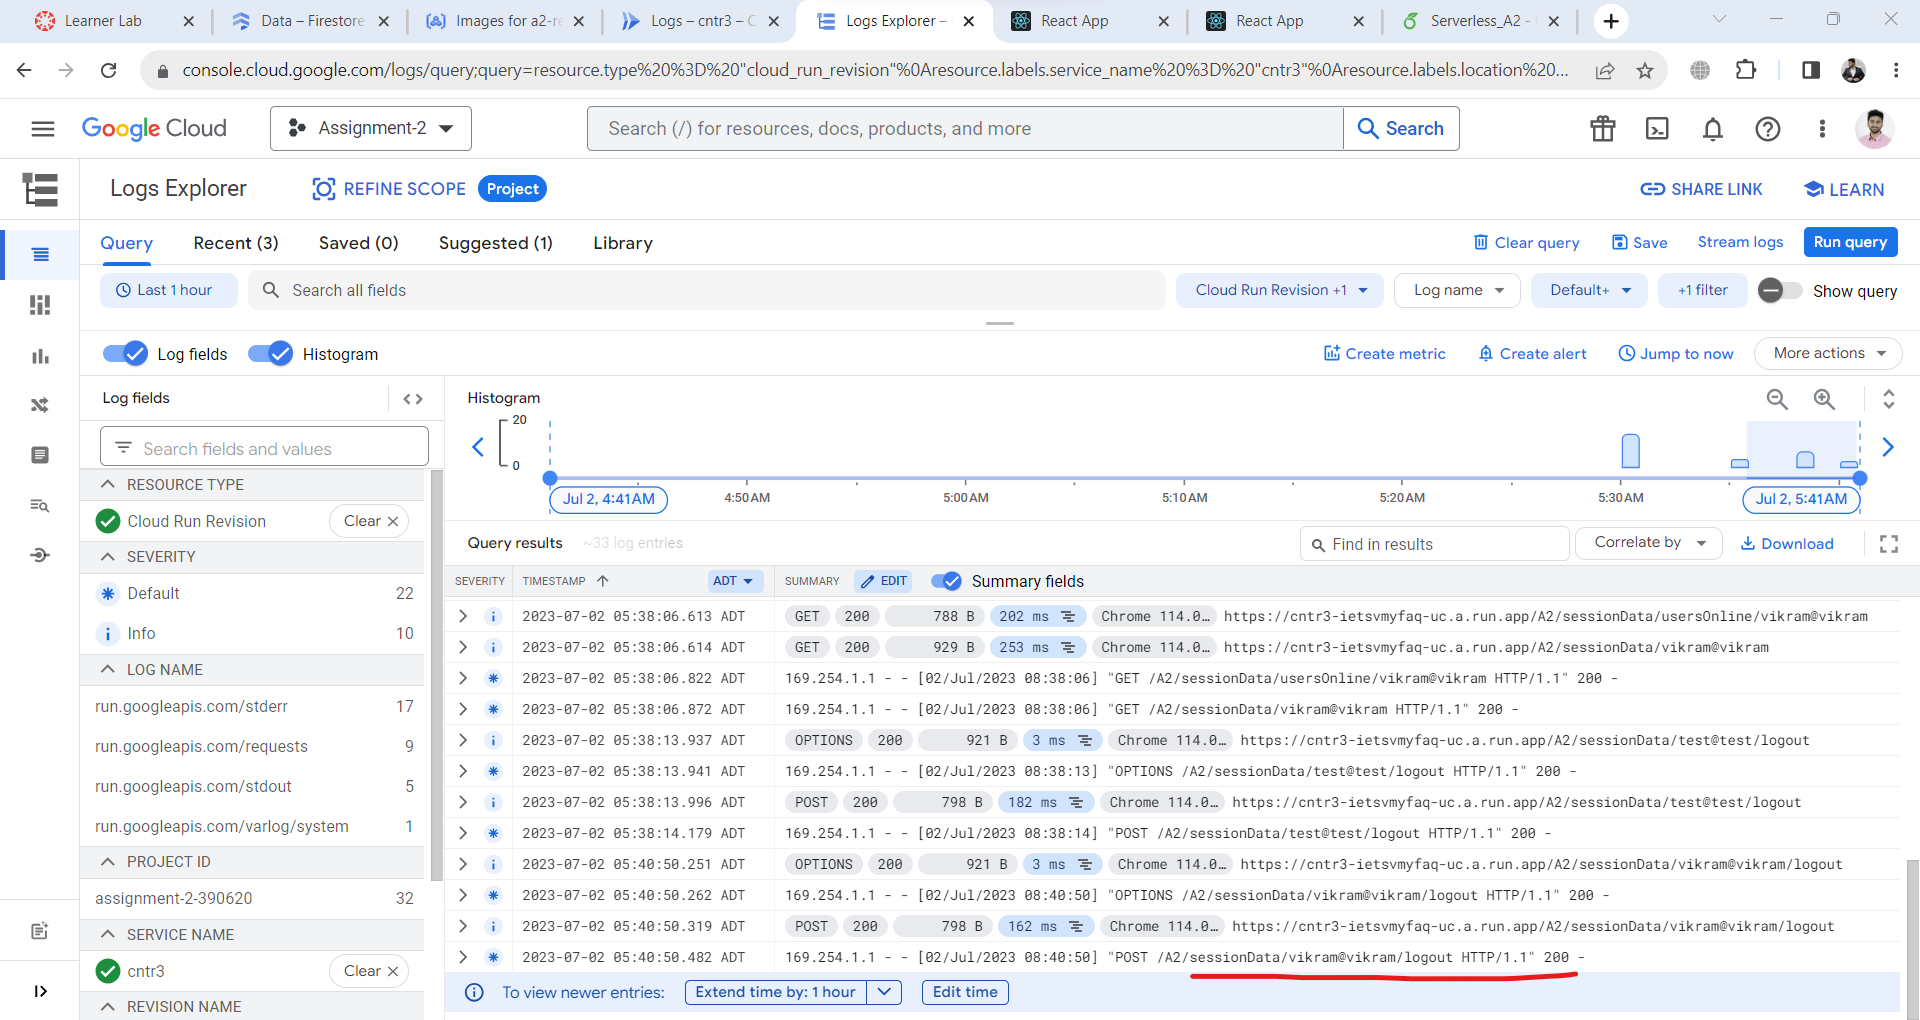
\includegraphics[scale=1, width=15cm,height=7.5cm]{PROBLEM 2/Screenshots/2. Demo/1. Logs/5. vikram session logout.png}}
    \caption{\textbf{\textit{User - Vikram: Logout logs}}}
    \label{fig:vikram-logout-success}
\end{figure}
\begin{figure}[htp]
    \centering
    \fbox{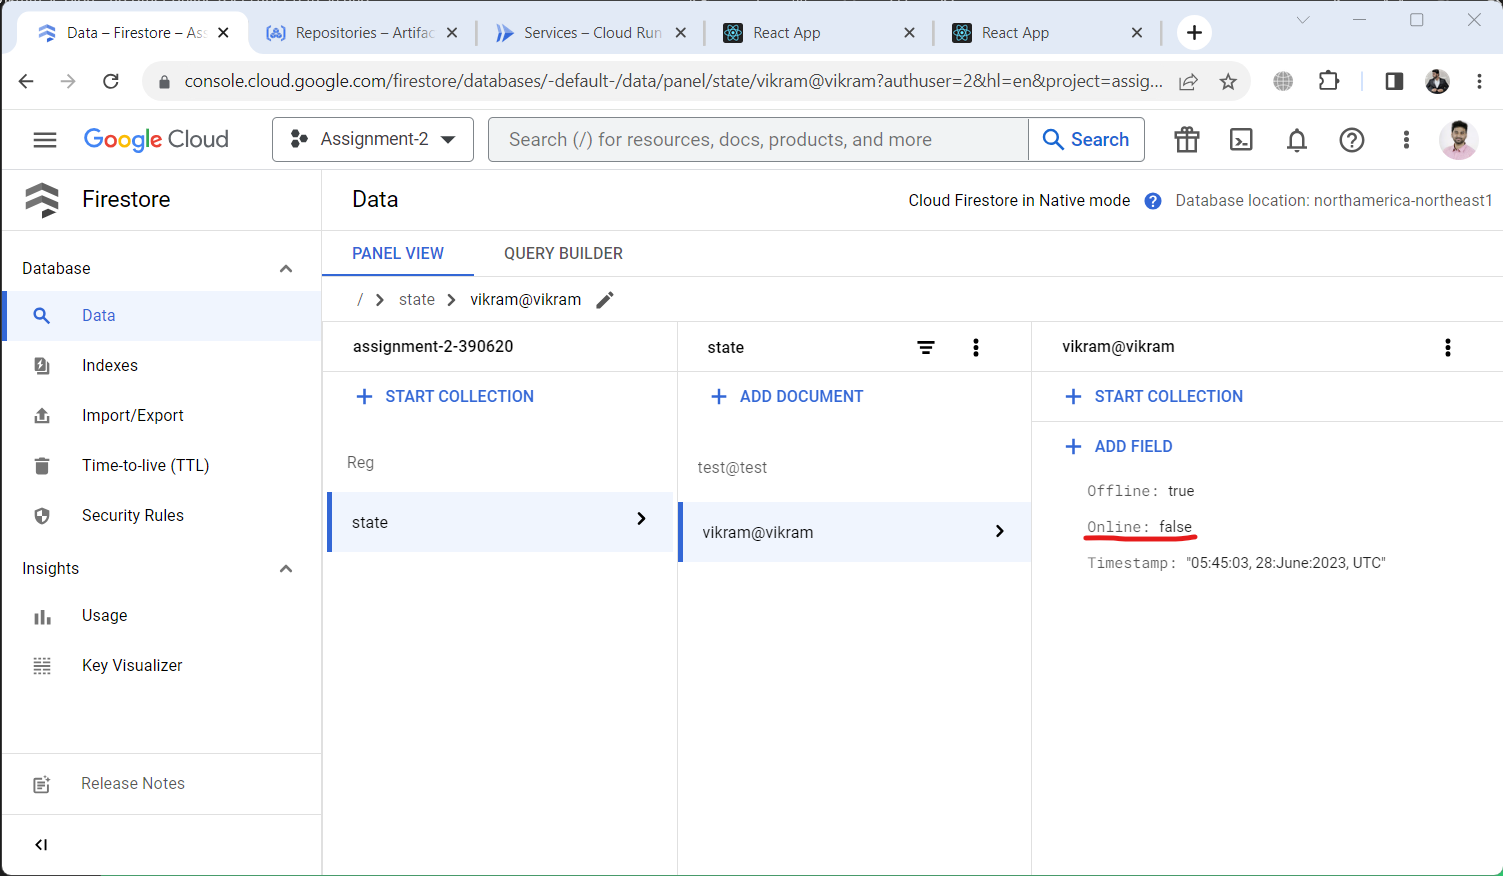
\includegraphics[scale=1, width=15cm,height=7.5cm]{PROBLEM 2/Screenshots/2. Demo/7.3 vikram session - offline after logout.png}}
    \caption{\textbf{\textit{User - Vikram: Session is offline}}}
    \label{fig:vikram-session-offline}
\end{figure}

\newpage\newpage
\section{Test cases}
\begin{figure}[htp]
    \centering
    \fbox{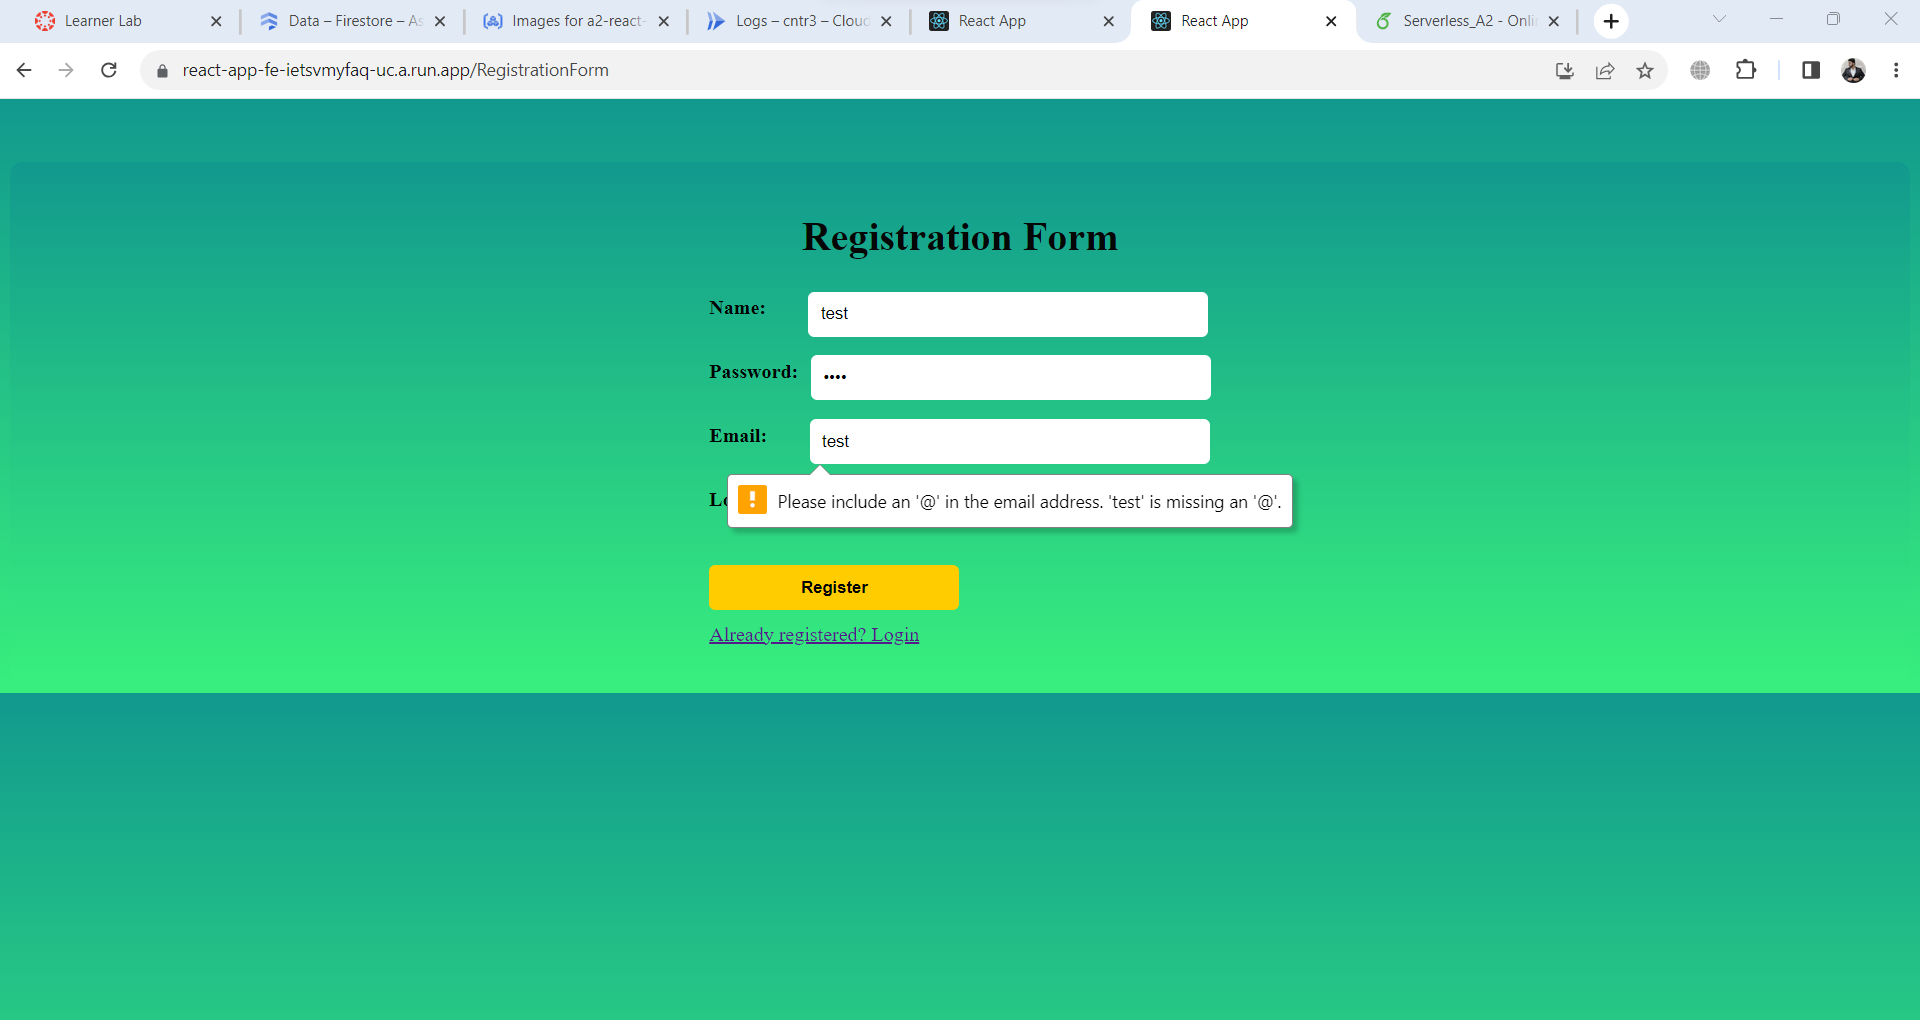
\includegraphics[scale=1, width=15cm,height=7.5cm]{PROBLEM 2/Screenshots/4. Test case/0. email needs @.png}}
    \caption{\textbf{\textit{Email validation - must have '@' symbol}}}
    \label{fig:test-case-invalid-creds}
\end{figure}
\begin{figure}[htp]
    \centering
    \fbox{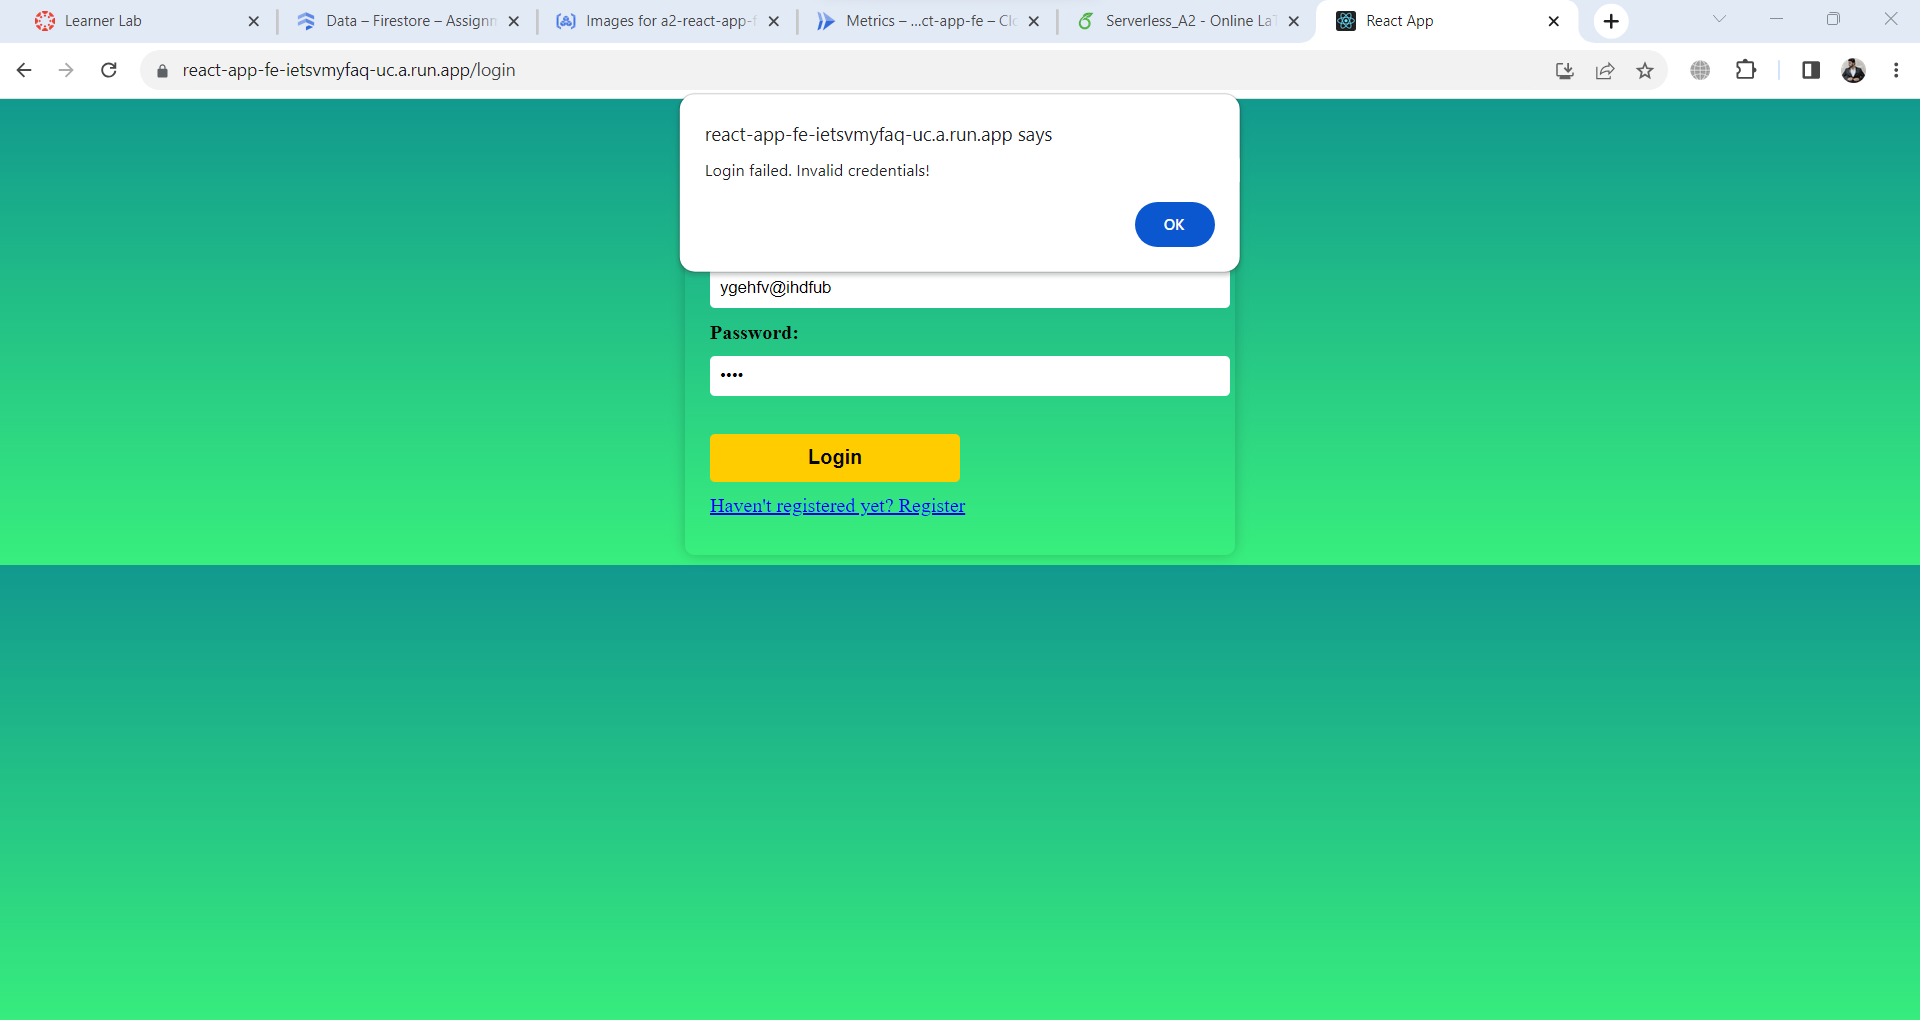
\includegraphics[scale=1, width=15cm,height=7.5cm]{PROBLEM 2/Screenshots/4. Test case/1. invalid credentials.png}}
    \caption{\textbf{\textit{Input: random credentials, Error: "Invalid credentials" - Since the record is not present in the collection "Reg"}}}
    \label{fig:test-case-invalid-creds}
\end{figure}
\begin{figure}[htp]
    \centering
    \fbox{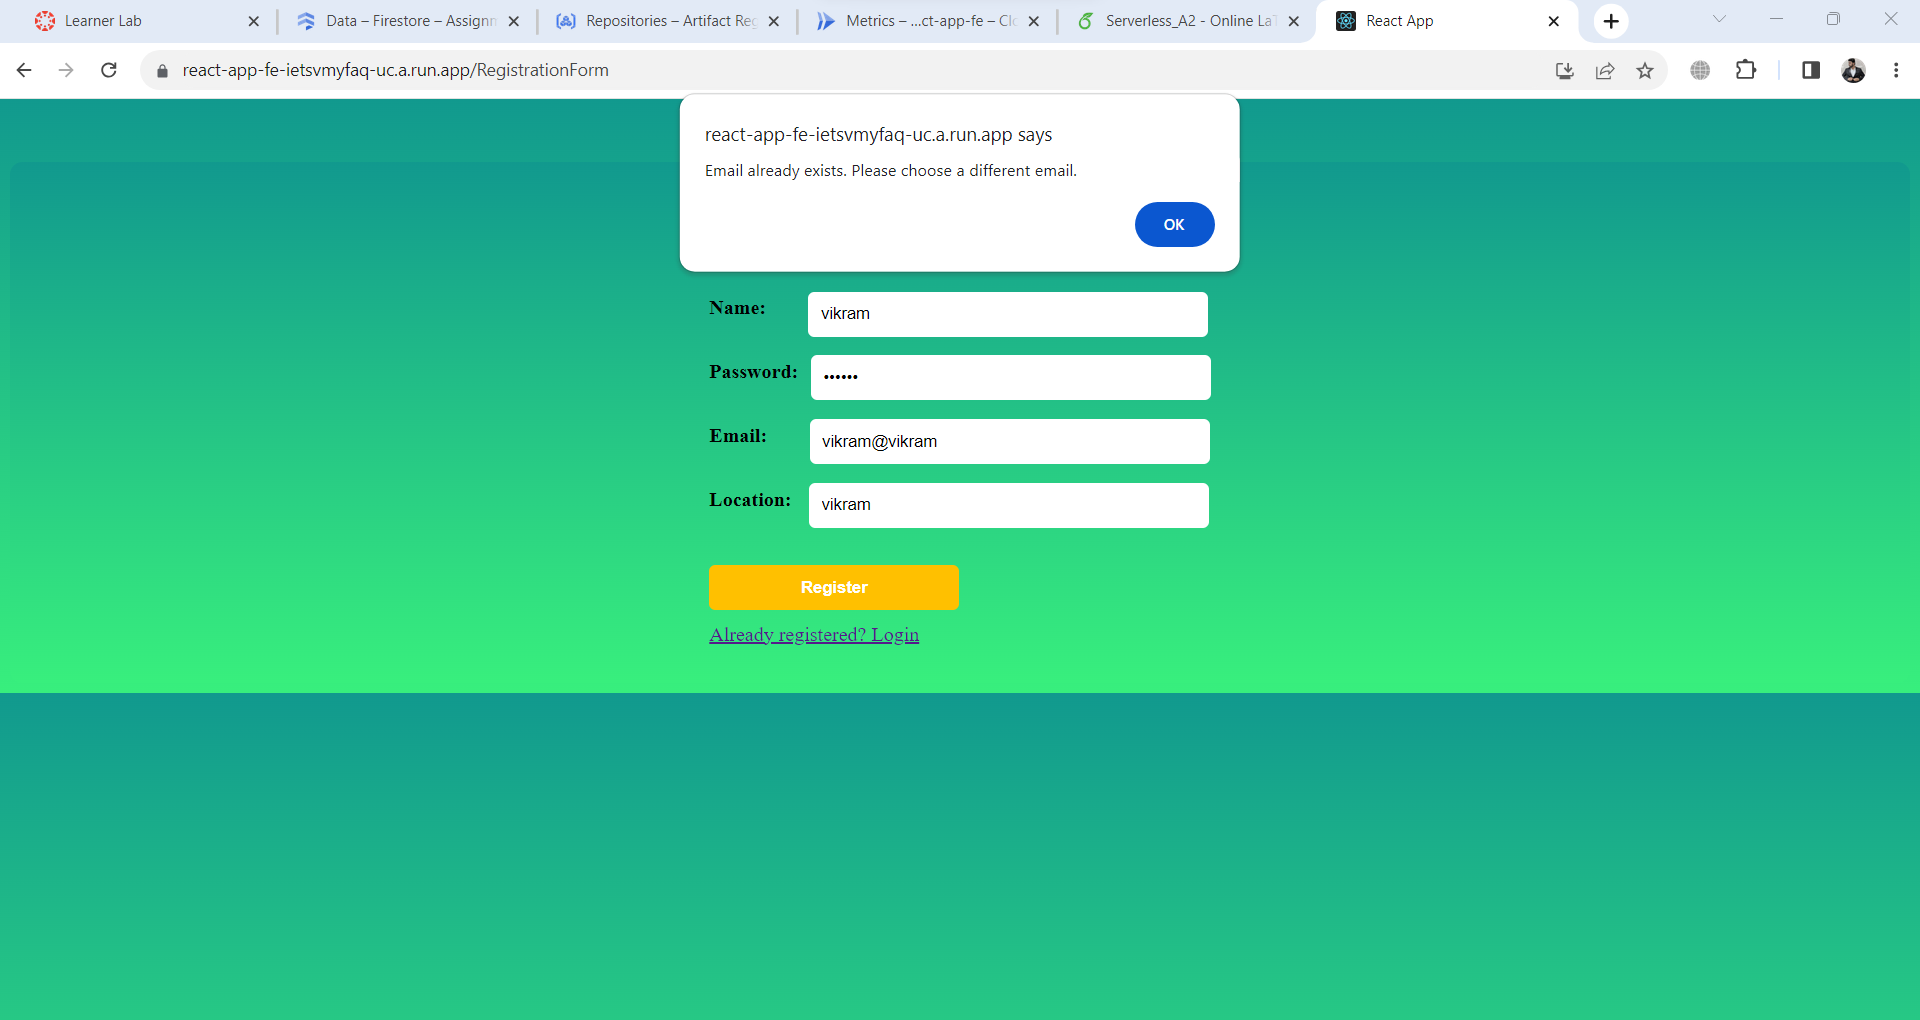
\includegraphics[scale=1, width=15cm,height=7.5cm]{PROBLEM 2/Screenshots/4. Test case/2. email already exists.png}}
    \caption{\textbf{\textit{Input: registration with an already existing email. Error: "Email already exists" - indicating that the entered email is already present in the collection "Reg"}}}
    \label{fig:test-case-email-exists}
\end{figure}

\begin{figure}[htp]
    \centering
    \fbox{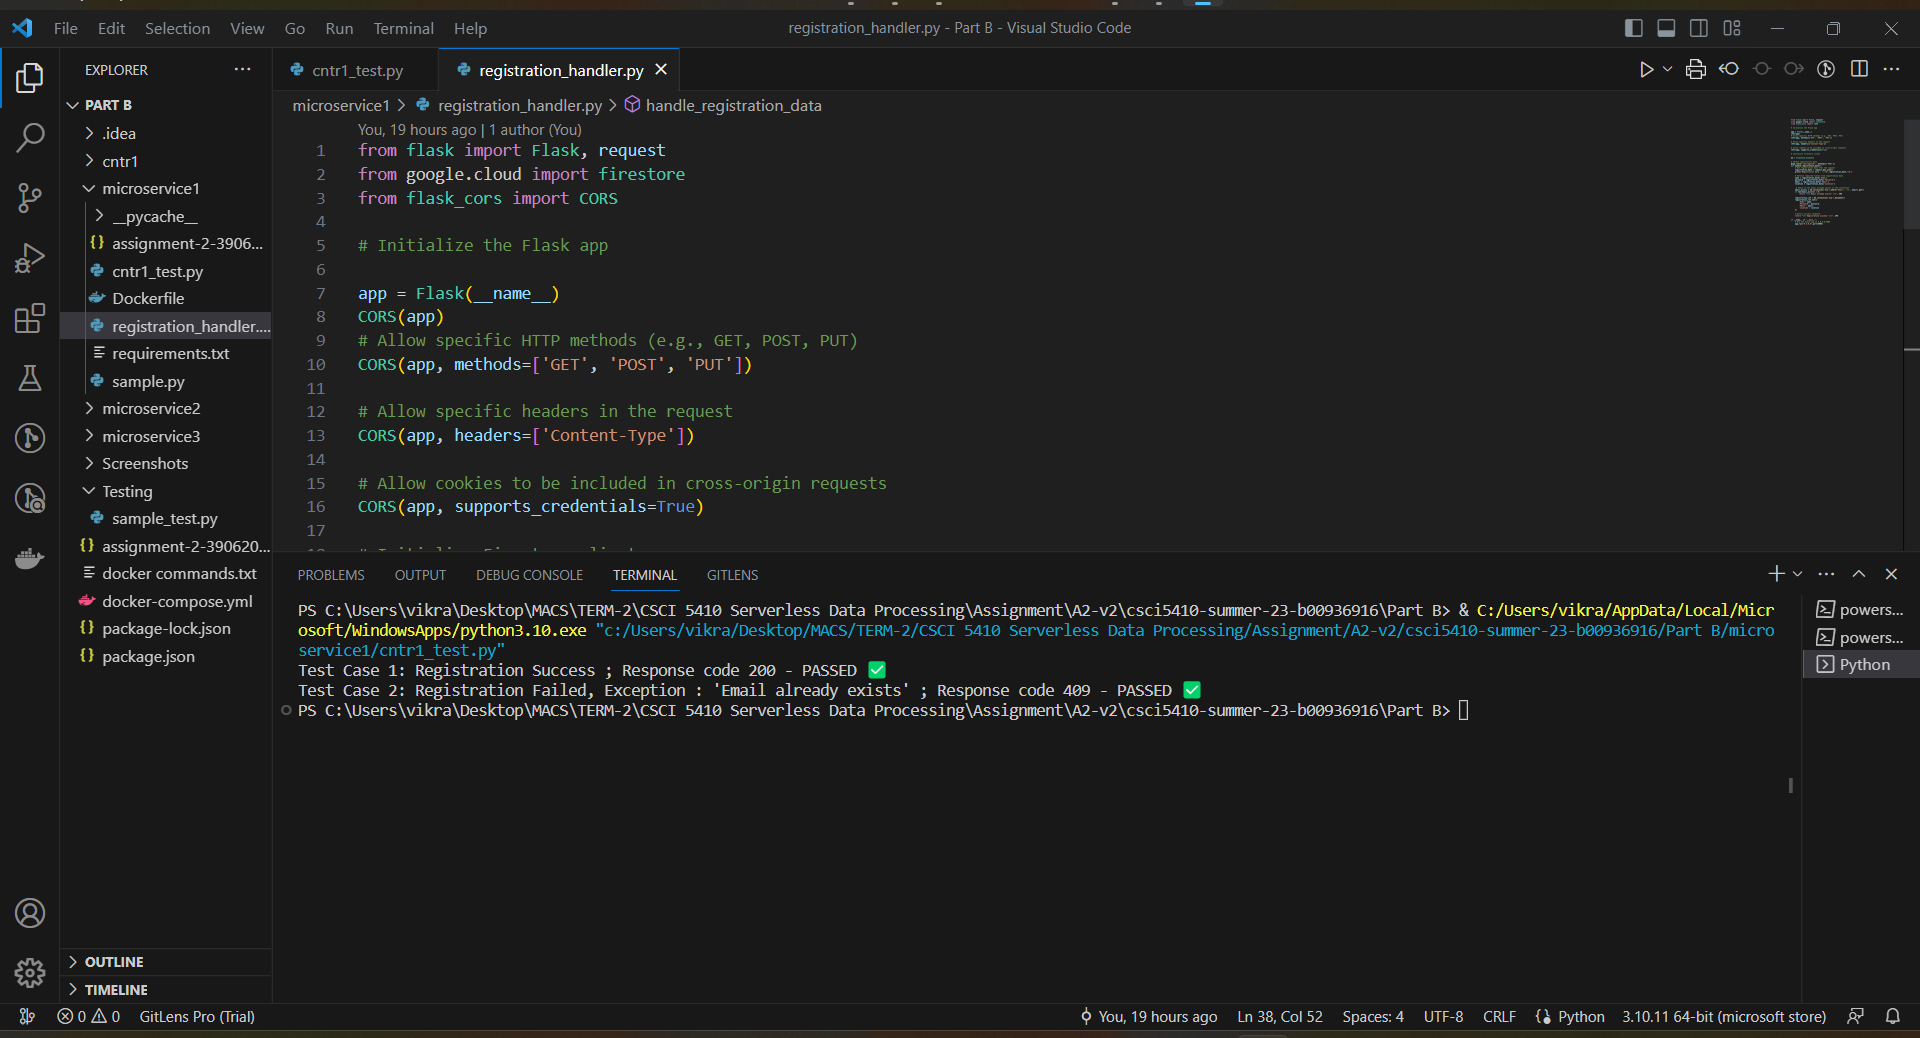
\includegraphics[scale=1, width=15cm,height=7.5cm]{PROBLEM 2/Screenshots/4. Test case/Backend/1. cntr1 test cases passed.png}}
    \caption{\textbf{\textit{Test cases for container 1}}}
    \label{fig:test-case-container-1}
\end{figure}

\begin{figure}[htp]
    \centering
    \fbox{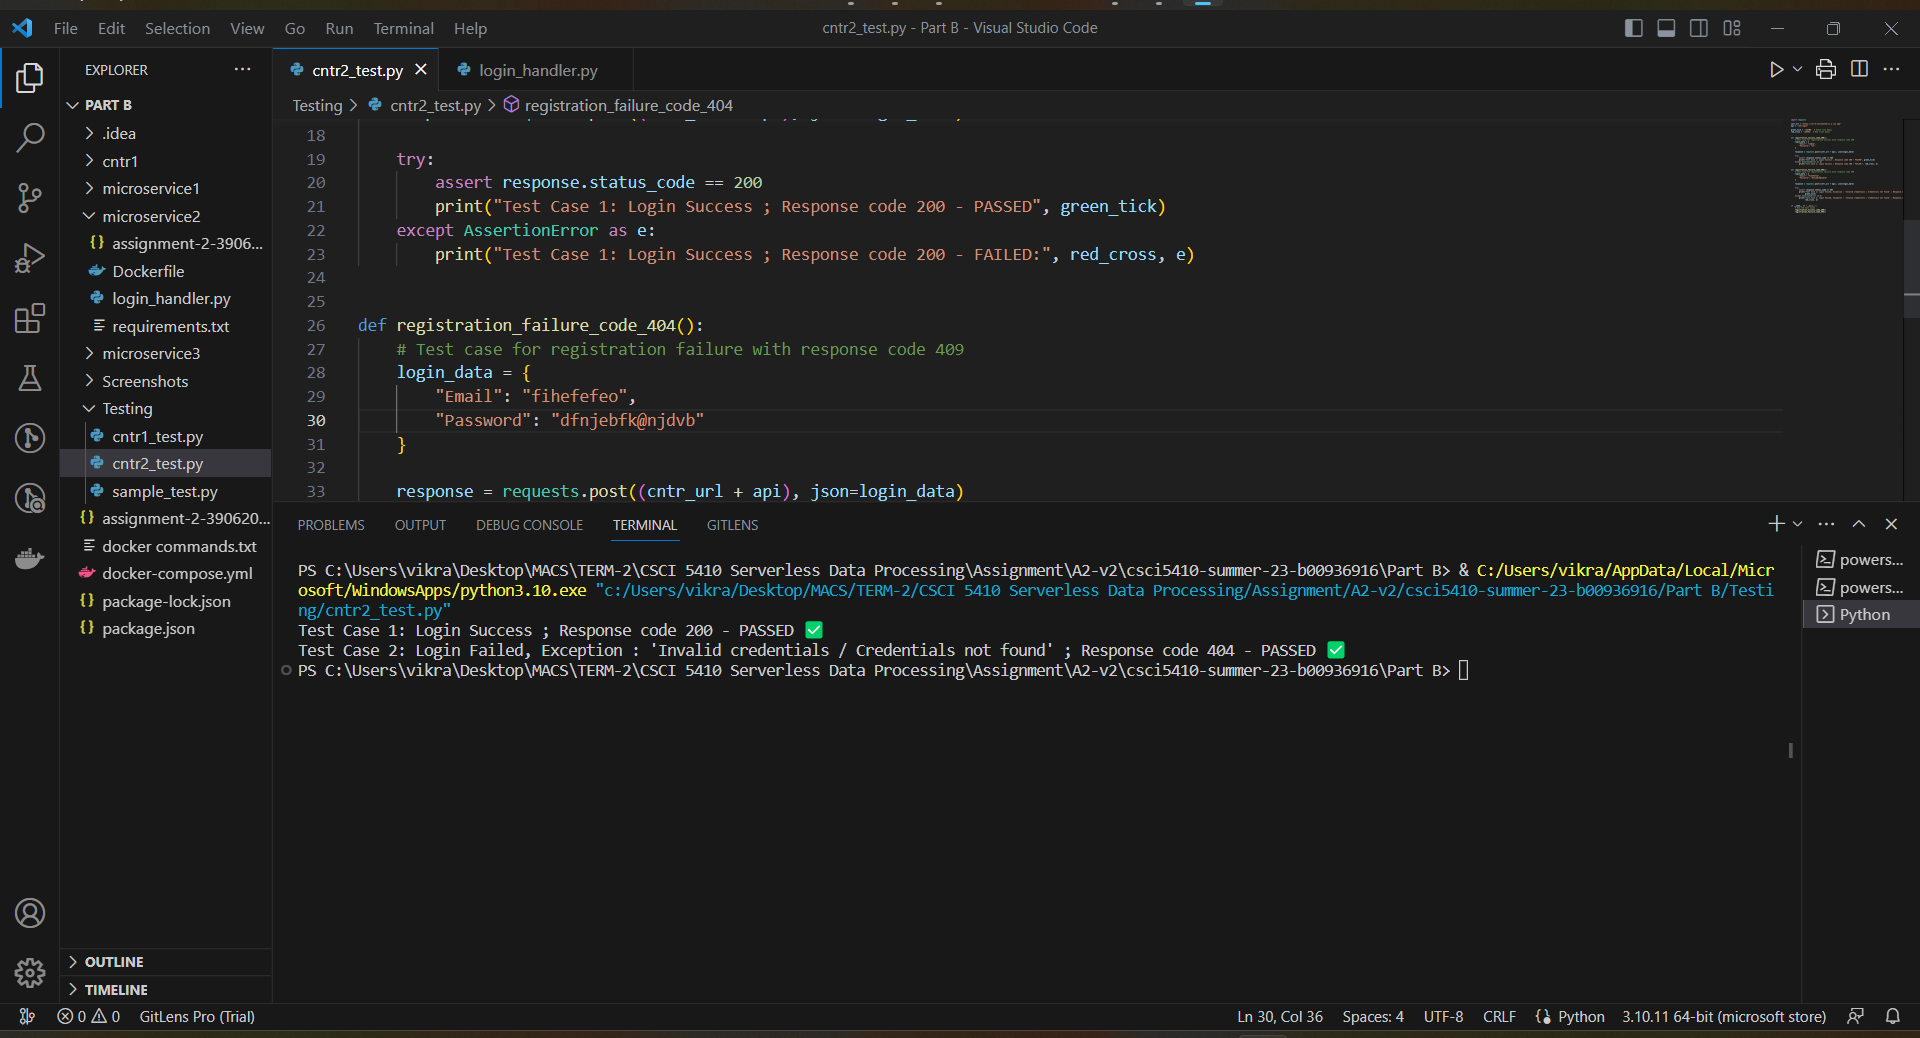
\includegraphics[scale=1, width=15cm,height=7.5cm]{PROBLEM 2/Screenshots/4. Test case/Backend/2. cntr2 test cases passed.png}}
    \caption{\textbf{\textit{Test cases for container 2}}}
    \label{fig:test-case-container-2}
\end{figure}

\begin{figure}[htp]
    \centering
    \fbox{\includegraphics[scale=1, width=15cm,height=7.5cm]{PROBLEM 2/Screenshots/4. Test case/Backend/3. cntr3 session data passed.png}}
    \caption{\textbf{\textit{Test cases for container 3}}}
    \label{fig:test-case-container-3}
\end{figure}

\newpage
\section{My view on leveraging Google Cloud Run, GCR/Artifact Registry, and Docker Containers for Efficient Application Deployment}

My application relies on the power of Google Cloud technologies to achieve seamless deployment and management. By utilizing Google Cloud Run[3], I can deploy my application as stateless containers, benefitting from automatic scaling and secure execution. This allows me to focus on developing my application code while leaving the infrastructure complexities to Cloud Run.
\newline\newline
To store and manage my container images, I utilized Google Artifact Registry[2]. This central repository enabled me to version control my images, control access to containers, and efficiently distribute them across different environments. With easy push and pull capabilities[8], I can ensure smooth deployment and updates[7] of my container images.
\newline\newline
Docker containers[6] play a vital role in the deployment process. They encapsulate the application code, dependencies, and configurations, making deployments consistent and portable. Docker's containerization technology provides isolation, scalability, and optimized resource utilization, contributing to improved performance and maintainability of the application.
\newline\newline
 \textbf{My personal observation:}
 \newline
During the process of pushing Docker images to Artifact Registry, I observed an interesting behavior. When pushing the "cnt2" images, I noticed that instead of uploading all the layers from scratch, the system fetched some layers from the previously pushed "cntr1" images (Refer figures \ref{fig:push-container-1},\ref{fig:push-container-2},\ref{fig:push-container-3}). Since these layers were identical, reusing them saved valuable time and resources. This optimization in the image pushing process demonstrates the efficiency of Google Artifact Registry in handling and managing container images, further enhancing the overall deployment experience.
\newline\newline
In conclusion, my application benefits from Google Cloud Run's scalability, Artifact Registry's image management capabilities, and Docker containers' consistency and portability. These technologies work harmoniously to provide me with an efficient, secure, and easily manageable application infrastructure. Additionally, Docker and Google Cloud Platform offer extensive documentation and resources, which enabled me to maximize the benefits of these tools in my application development and deployment process.









% \begin{figure}[htp]
%     \centering
%     \fbox{\includegraphics[scale=1, width=15cm,height=7.5cm]{PROBLEM 2/}
%     \caption{\textbf{\textit{ }}}}
%     \label{fig:}
% \end{figure}


\newpage
\appendix

\part{REFERENCES}

\section*{References}
\begin{sloppypar}

  \begin{enumerate}[label={[\arabic*]}]
  
    \item N. Naik, "Performance Evaluation of Distributed Systems in Multiple Clouds using Docker Swarm," 2021 \textit{IEEE International Systems Conference (SysCon)}, Vancouver, BC, Canada, 2021, pp. 1-6, doi: 10.1109/SysCon48628.2021.9447123

    \item “Create standard repositories,” \textit{Google Cloud}. [Online]. Available: https://cloud.google.com/artifact-registry/docs/repositories/create-repos.[Accessed: 29 June 2023].

    \item “Deploying to cloud run,” \textit{Google Cloud}. [Online]. Available: https://cloud.google.com/run/docs/deploying. [Accessed: 29 June 2023].

    \item “Add data to cloud firestore,” \textit{Firebase}. [Online]. Available: https://firebase.google.com/docs/firestore/manage-data/add-data. [Accessed: 29 June 2023].

    \item “Get data with cloud firestore,” \textit{Firebase}. [Online]. Available: https://firebase.google.com/docs/firestore/query-data/get-data. [Accessed: 29 June 2023].

    \item “Containerize an application,” \textit{Docker Documentation}, 28-Jun-2023. [Online]. Available: https://docs.docker.com/get-started/02\_our\_app/. [Accessed: 29 June 2023].


    \item	“Update the application,”\textit{ Docker Documentation}, 28-Jun-2023. [Online]. Available: https://docs.docker.com/get-started/03\_updating\_app/. [Accessed: 29 June 2023].


    \item “Push and pull images,”\textit{ Google Cloud}. [Online]. Available: https://cloud.google.com/artifact-registry/docs/docker/pushing-and-pulling. [Accessed: 29 June 2023].


    \item “Create a new react app,” \textit{Reactjs.org}. [Online]. Available: https://legacy.reactjs.org/docs/create-a-new-react-app.html. [Accessed: 29 June 2023].


    \item	S.Gandotra, “ReactJS router,” \textit{GeeksforGeeks}, 13-Dec-2019. [Online]. Available: https://www.geeksforgeeks.org/reactjs-router/. [Accessed: 29 June 2023].
    
    \item "LaTeX Listings package JSON formatting," \textit{TeX Stack Exchange}, Available: https://tex.stackexchange.com/questions/560830/latex-listings-package-json-formatting. [Accessed 29 June 2023].
    
    \item V. Venkatapathi, "B00936916_VikramVenkatapathi_A1_Report.pdf," \textit{Dalhousie University}, Jan. 2023. [Online]. Available: https://git.cs.dal.ca/vikramv/csci5408_w23_b00936916_vikram_venkatapathi/-/blob/main/Assignment_1/B00936916_VikramVenkatapathi_A1_Report.pdf. [Accessed 29 June 2023].
    
    \item Shanmuganathan, Vishakan. "OOAD-Project." \textit{GitHub}, 2021, https://github.com/svishakan/OOAD-Project. [Accessed 29 June 2023].

    \item AWS. "Amazon Lex V1",\textit{Amazon.com}[Online]. Available: https://docs.aws.amazon.com/lex/latest/dg/gs-bp-create-bot.html. [Accessed: 29 June 2023].

    \item “Swarm mode overview,” \textit{Docker Documentation}, 30-Jun-2023. [Online]. Available: https://docs.docker.com/engine/swarm/. [Accessed: 03 July 2023].

    \item R. Powell, “Docker Swarm vs Kubernetes: how to choose a container orchestration tool,” \textit{CircleCI}, 12-Oct-2021. [Online]. Available: https://circleci.com/blog/docker-swarm-vs-kubernetes/. [Accessed: 03 July 2023].

    \item “Production-Grade Container Orchestration,” \textit{Kubernetes}. [Online]. Available: https://kubernetes.io/. [Accessed: 03 July 2023].

    \item “Lightweight kubernetes,” \textit{K3s.io}. [Online]. Available: https://k3s.io/. [Accessed: 03 July 2023].

  \end{enumerate}

\end{sloppypar}
\newpage


% \bibliographystyle{IEEEtran}
% \bibliography{REFERENCES/references}
\end{document}
